% This is the Reed College LaTeX thesis template. Most of the work
% for the document class was done by Sam Noble (SN), as well as this
% template. Later comments etc. by Ben Salzberg (BTS). Additional
% restructuring and APA support by Jess Youngberg (JY).
% Your comments and suggestions are more than welcome; please email
% them to cus@reed.edu
%
% See https://www.reed.edu/cis/help/LaTeX/index.html for help. There are a
% great bunch of help pages there, with notes on
% getting started, bibtex, etc. Go there and read it if you're not
% already familiar with LaTeX.
%
% Any line that starts with a percent symbol is a comment.
% They won't show up in the document, and are useful for notes
% to yourself and explaining commands.
% Commenting also removes a line from the document;
% very handy for troubleshooting problems. -BTS

% As far as I know, this follows the requirements laid out in
% the 2002-2003 Senior Handbook. Ask a librarian to check the
% document before binding. -SN

%%
%% Preamble
%%
% \documentclass{<something>} must begin each LaTeX document
\documentclass[12pt,twoside]{reedthesis}
% Packages are extensions to the basic LaTeX functions. Whatever you
% want to typeset, there is probably a package out there for it.
% Chemistry (chemtex), screenplays, you name it.
% Check out CTAN to see: https://www.ctan.org/
%%
\usepackage{graphicx,latexsym}
\usepackage{amsmath}
\usepackage{amssymb,amsthm}
\usepackage{longtable,booktabs,setspace}
\usepackage{chemarr} %% Useful for one reaction arrow, useless if you're not a chem major
\usepackage[hyphens]{url}
% Added by CII
\usepackage{hyperref}
\usepackage{lmodern}
\usepackage{float}
\floatplacement{figure}{H}
% End of CII addition
\usepackage{rotating}

% Next line commented out by CII
%%% \usepackage{natbib}
% Comment out the natbib line above and uncomment the following two lines to use the new
% biblatex-chicago style, for Chicago A. Also make some changes at the end where the
% bibliography is included.
%\usepackage{biblatex-chicago}
%\bibliography{thesis}


% Added by CII (Thanks, Hadley!)
% Use ref for internal links
\renewcommand{\hyperref}[2][???]{\autoref{#1}}
\def\chapterautorefname{Chapter}
\def\sectionautorefname{Section}
\def\subsectionautorefname{Subsection}
% End of CII addition

% Added by CII
\usepackage{caption}
\captionsetup{width=5in}
% End of CII addition

% \usepackage{times} % other fonts are available like times, bookman, charter, palatino

% Syntax highlighting #22
  \usepackage{color}
  \usepackage{fancyvrb}
  \newcommand{\VerbBar}{|}
  \newcommand{\VERB}{\Verb[commandchars=\\\{\}]}
  \DefineVerbatimEnvironment{Highlighting}{Verbatim}{commandchars=\\\{\}}
  % Add ',fontsize=\small' for more characters per line
  \usepackage{framed}
  \definecolor{shadecolor}{RGB}{248,248,248}
  \newenvironment{Shaded}{\begin{snugshade}}{\end{snugshade}}
  \newcommand{\AlertTok}[1]{\textcolor[rgb]{0.94,0.16,0.16}{#1}}
  \newcommand{\AnnotationTok}[1]{\textcolor[rgb]{0.56,0.35,0.01}{\textbf{\textit{#1}}}}
  \newcommand{\AttributeTok}[1]{\textcolor[rgb]{0.77,0.63,0.00}{#1}}
  \newcommand{\BaseNTok}[1]{\textcolor[rgb]{0.00,0.00,0.81}{#1}}
  \newcommand{\BuiltInTok}[1]{#1}
  \newcommand{\CharTok}[1]{\textcolor[rgb]{0.31,0.60,0.02}{#1}}
  \newcommand{\CommentTok}[1]{\textcolor[rgb]{0.56,0.35,0.01}{\textit{#1}}}
  \newcommand{\CommentVarTok}[1]{\textcolor[rgb]{0.56,0.35,0.01}{\textbf{\textit{#1}}}}
  \newcommand{\ConstantTok}[1]{\textcolor[rgb]{0.00,0.00,0.00}{#1}}
  \newcommand{\ControlFlowTok}[1]{\textcolor[rgb]{0.13,0.29,0.53}{\textbf{#1}}}
  \newcommand{\DataTypeTok}[1]{\textcolor[rgb]{0.13,0.29,0.53}{#1}}
  \newcommand{\DecValTok}[1]{\textcolor[rgb]{0.00,0.00,0.81}{#1}}
  \newcommand{\DocumentationTok}[1]{\textcolor[rgb]{0.56,0.35,0.01}{\textbf{\textit{#1}}}}
  \newcommand{\ErrorTok}[1]{\textcolor[rgb]{0.64,0.00,0.00}{\textbf{#1}}}
  \newcommand{\ExtensionTok}[1]{#1}
  \newcommand{\FloatTok}[1]{\textcolor[rgb]{0.00,0.00,0.81}{#1}}
  \newcommand{\FunctionTok}[1]{\textcolor[rgb]{0.00,0.00,0.00}{#1}}
  \newcommand{\ImportTok}[1]{#1}
  \newcommand{\InformationTok}[1]{\textcolor[rgb]{0.56,0.35,0.01}{\textbf{\textit{#1}}}}
  \newcommand{\KeywordTok}[1]{\textcolor[rgb]{0.13,0.29,0.53}{\textbf{#1}}}
  \newcommand{\NormalTok}[1]{#1}
  \newcommand{\OperatorTok}[1]{\textcolor[rgb]{0.81,0.36,0.00}{\textbf{#1}}}
  \newcommand{\OtherTok}[1]{\textcolor[rgb]{0.56,0.35,0.01}{#1}}
  \newcommand{\PreprocessorTok}[1]{\textcolor[rgb]{0.56,0.35,0.01}{\textit{#1}}}
  \newcommand{\RegionMarkerTok}[1]{#1}
  \newcommand{\SpecialCharTok}[1]{\textcolor[rgb]{0.00,0.00,0.00}{#1}}
  \newcommand{\SpecialStringTok}[1]{\textcolor[rgb]{0.31,0.60,0.02}{#1}}
  \newcommand{\StringTok}[1]{\textcolor[rgb]{0.31,0.60,0.02}{#1}}
  \newcommand{\VariableTok}[1]{\textcolor[rgb]{0.00,0.00,0.00}{#1}}
  \newcommand{\VerbatimStringTok}[1]{\textcolor[rgb]{0.31,0.60,0.02}{#1}}
  \newcommand{\WarningTok}[1]{\textcolor[rgb]{0.56,0.35,0.01}{\textbf{\textit{#1}}}}

% To pass between YAML and LaTeX the dollar signs are added by CII
\title{A Hierarchical Bayesian Approach to Small Area Estimation of Forest Attributes}
\author{Grayson White}
% The month and year that you submit your FINAL draft TO THE LIBRARY (May or December)
\date{May 2021}
\division{Mathematics and Natural Sciences}
\advisor{Kelly McConville}
\institution{Reed College}
\degree{Bachelor of Arts}
%If you have two advisors for some reason, you can use the following
% Uncommented out by CII
% End of CII addition

%%% Remember to use the correct department!
\department{Mathematics}
% if you're writing a thesis in an interdisciplinary major,
% uncomment the line below and change the text as appropriate.
% check the Senior Handbook if unsure.
%\thedivisionof{The Established Interdisciplinary Committee for}
% if you want the approval page to say "Approved for the Committee",
% uncomment the next line
%\approvedforthe{Committee}

% Added by CII
%%% Copied from knitr
%% maxwidth is the original width if it's less than linewidth
%% otherwise use linewidth (to make sure the graphics do not exceed the margin)
\makeatletter
\def\maxwidth{ %
  \ifdim\Gin@nat@width>\linewidth
    \linewidth
  \else
    \Gin@nat@width
  \fi
}
\makeatother

%Added by @MyKo101, code provided by @GerbrichFerdinands

\renewcommand{\contentsname}{Table of Contents}
% End of CII addition

\setlength{\parskip}{0pt}

% Added by CII

\providecommand{\tightlist}{%
  \setlength{\itemsep}{0pt}\setlength{\parskip}{0pt}}

\Acknowledgements{
This is where acknowledgements will go.
}

\Dedication{
To my family.
}

\Preface{
This is an example of a thesis setup to use the reed thesis document class
(for LaTeX) and the R bookdown package, in general.
}

\Abstract{
The preface pretty much says it all.

\par

Second paragraph of abstract starts here.
}

% End of CII addition
%%
%% End Preamble
%%
%
\begin{document}

% Everything below added by CII
  \maketitle

\frontmatter % this stuff will be roman-numbered
\pagestyle{empty} % this removes page numbers from the frontmatter
  \begin{acknowledgements}
    This is where acknowledgements will go.
  \end{acknowledgements}
  \begin{preface}
    This is an example of a thesis setup to use the reed thesis document class
    (for LaTeX) and the R bookdown package, in general.
  \end{preface}
  \hypersetup{linkcolor=black}
  \setcounter{tocdepth}{2}
  \tableofcontents

  \listoftables

  \listoffigures
  \begin{abstract}
    The preface pretty much says it all.
    
    \par
    
    Second paragraph of abstract starts here.
  \end{abstract}
  \begin{dedication}
    To my family.
  \end{dedication}
\mainmatter % here the regular arabic numbering starts
\pagestyle{fancyplain} % turns page numbering back on

\hypertarget{introduction}{%
\chapter*{Introduction}\label{introduction}}
\addcontentsline{toc}{chapter}{Introduction}

This is the introduction to my thesis.

\hypertarget{context}{%
\chapter{Context}\label{context}}

National forest inventories such as the United States Forest Inventory and Analysis Program (FIA) monitor the status of a nation's forests by collecting data and estimating forest attributes such as basal area, above-ground biomass, tree count per acre, and net volume. Due to the sheer amount of forests in the United States, the FIA cannot collect the population data for these variables across the United States. Instead, they use a sampling design intended and well-suited for estimation over large geographic regions such as states. This sampling design works very well for estimation in large regions and maintains a reasonable cost of employing foresters to collect the samples. While this method works sufficiently for large areas, it has become an interest of national forest inventories such as the FIA to be able to provide reliable and efficient estimates of forest attributes in small domains such as ecological subsections (often referred to as eco-subsections) and counties. In particular, the FIA would like to have estimates with low variance in eco-subsections, however, the FIA only samples a small numbers of plots in these small areas. Currently, the FIA's standard approach to this problem is by using post-stratification. Post-stratification uses a weighted average of the forest attribute of interest and corrects for over- or under-sampling of forested land in the small area. While this estimator is unbiased and has lower variance than the mean, it does not reduce the variance enough for precise estimation at the eco-subsection level. The research goal of this thesis is to address this problem by using techniques which seek to minimize estimate variance while only introducing a small amount of bias. Having precise estimates of forest attributes at the eco-subsection level is crucial for educational programs and implementation of programs which seek to maintain the health of our forests.

In order to produce these estimates we must perform small area estimation. Small area estimation is a branch of survey statistics which includes techniques that allow us to estimate the value of parameters at a sub-population level. Typically in survey estimation, we are interested in doing inference at a population level, however we are sometimes interested in attaining estimates for sub-populations or ``small areas.'' We can visualize the process by considering an ecological province divided into three eco-subsections, each of which have sampled areas:
\begin{figure}

{\centering 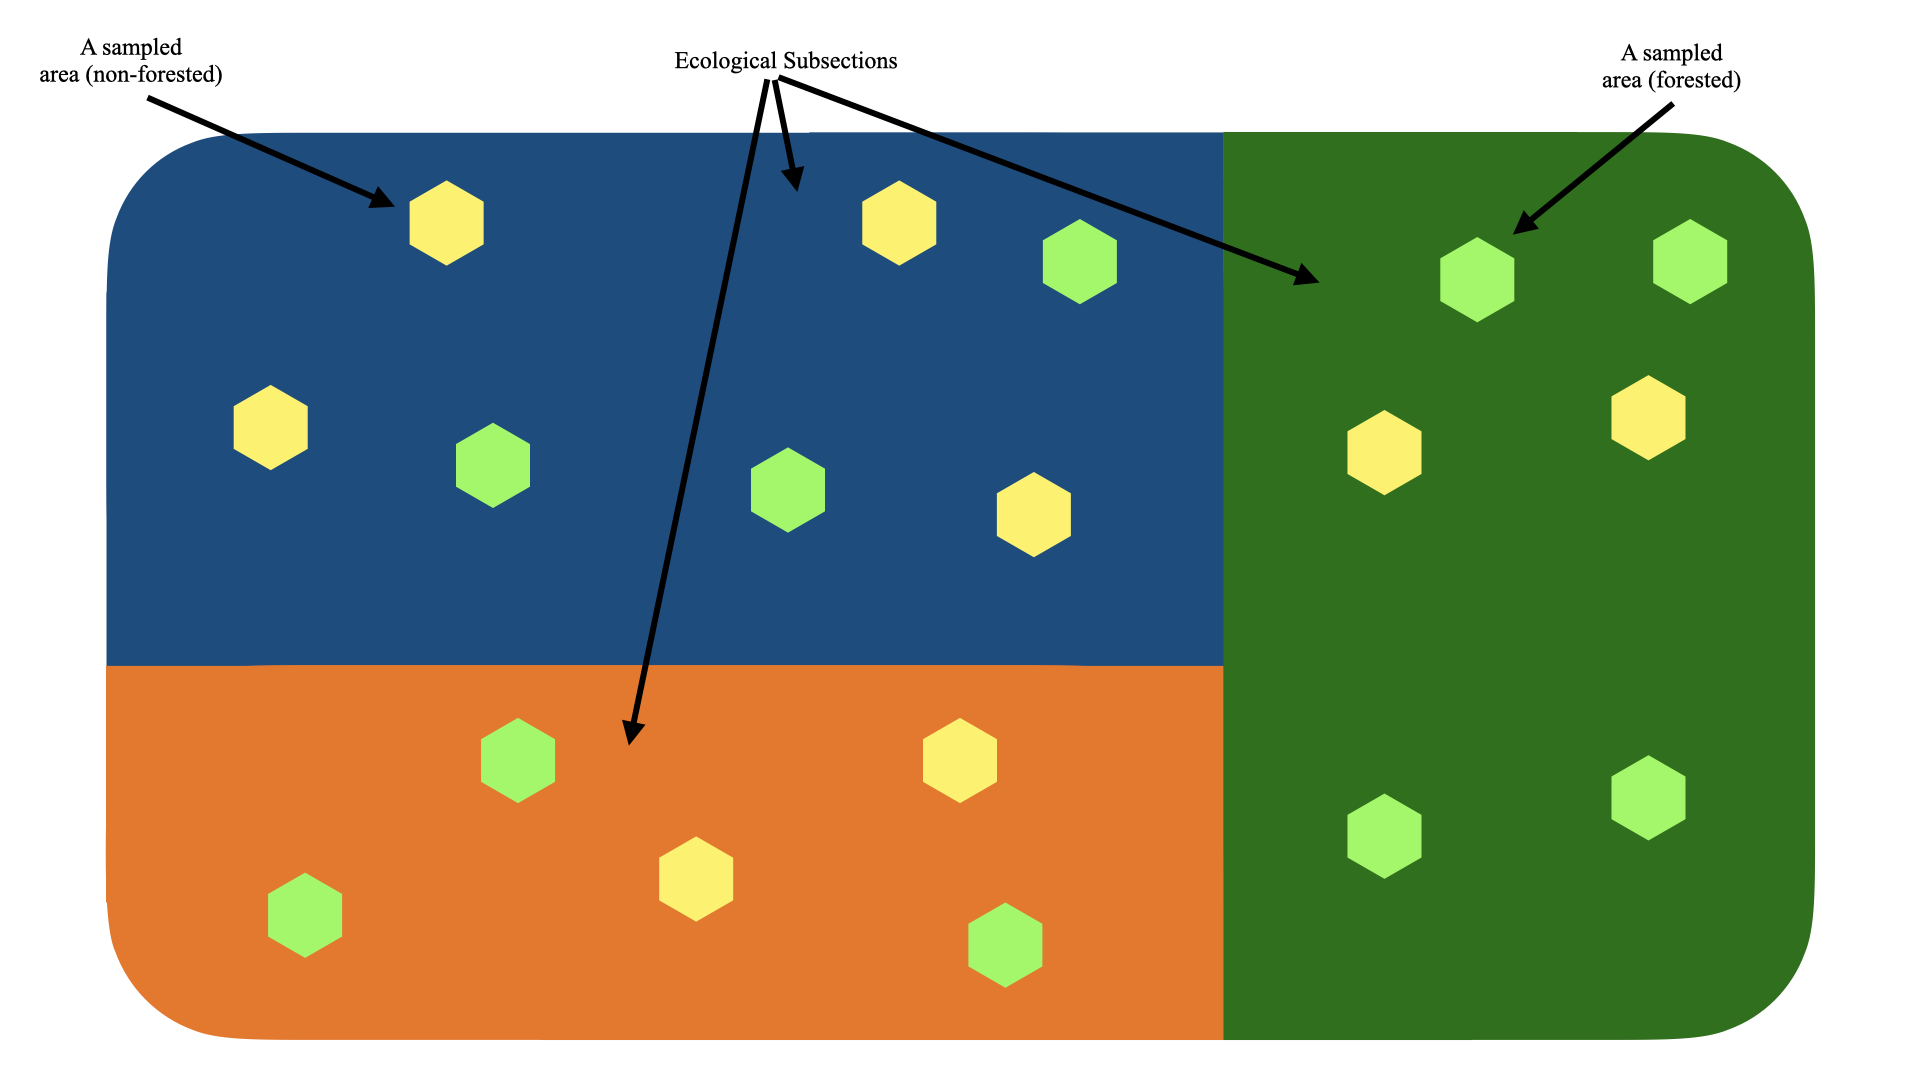
\includegraphics[width=1\linewidth]{figure/ecoprov-diagram} 

}

\caption[An ecological province]{An ecological province containing three eco-subsections. The red, yellow, and seafoam areas represent eco-subsections. The green hexagons represent forested areas sampled by the FIA. The beige hexagons represent non-forested areas sampled by the FIA.}\label{fig:ecological-province-diagram}
\end{figure}
We are interested in performing inference at the sub-population level, and in Figure \ref{fig:ecological-province-diagram} these sub-populations are represented by the red, yellow, and seafoam green areas. Importantly, we want to attain estimates of forest attributes in each of these sub-populations. There are wide range of techniques that can be used to carry out this small area estimation. Broadly, these methods fall into three categories: direct estimators, indirect estimators with implicit models, and indirect estimators with explicit models. We will often refer to indirect models with explicit models as ``model-based estimators.'' Each of these methods attempts to do inference at the sub-population level, however, they are quite different from each other.

Direct estimators are defined as those that rely only on the samples within the small area which we would like to measure. Some examples of a direct estimator are the sample mean or the post-stratified estimator. The post-stratified estimator is similar to the mean, however it accounts for under- and over-sampling of forested areas in a given sub-population. These estimators do not rely on information outside of the small area being estimated, however, the post-stratified estimator uses auxiliary information such as the true proportion of forested land within the small area to produce estimates. Direct estimation is the simplest kind of small area estimator as it only relies on samples within the sub-population of interest to produce its estimates. We can visualize these two estimators to get a better sense of their estimation process by considering how they would estimate some forest attribute \(y\) in our seafoam green sub-population \(j\) from Figure \ref{fig:ecological-province-diagram}.
\begin{figure}

{\centering 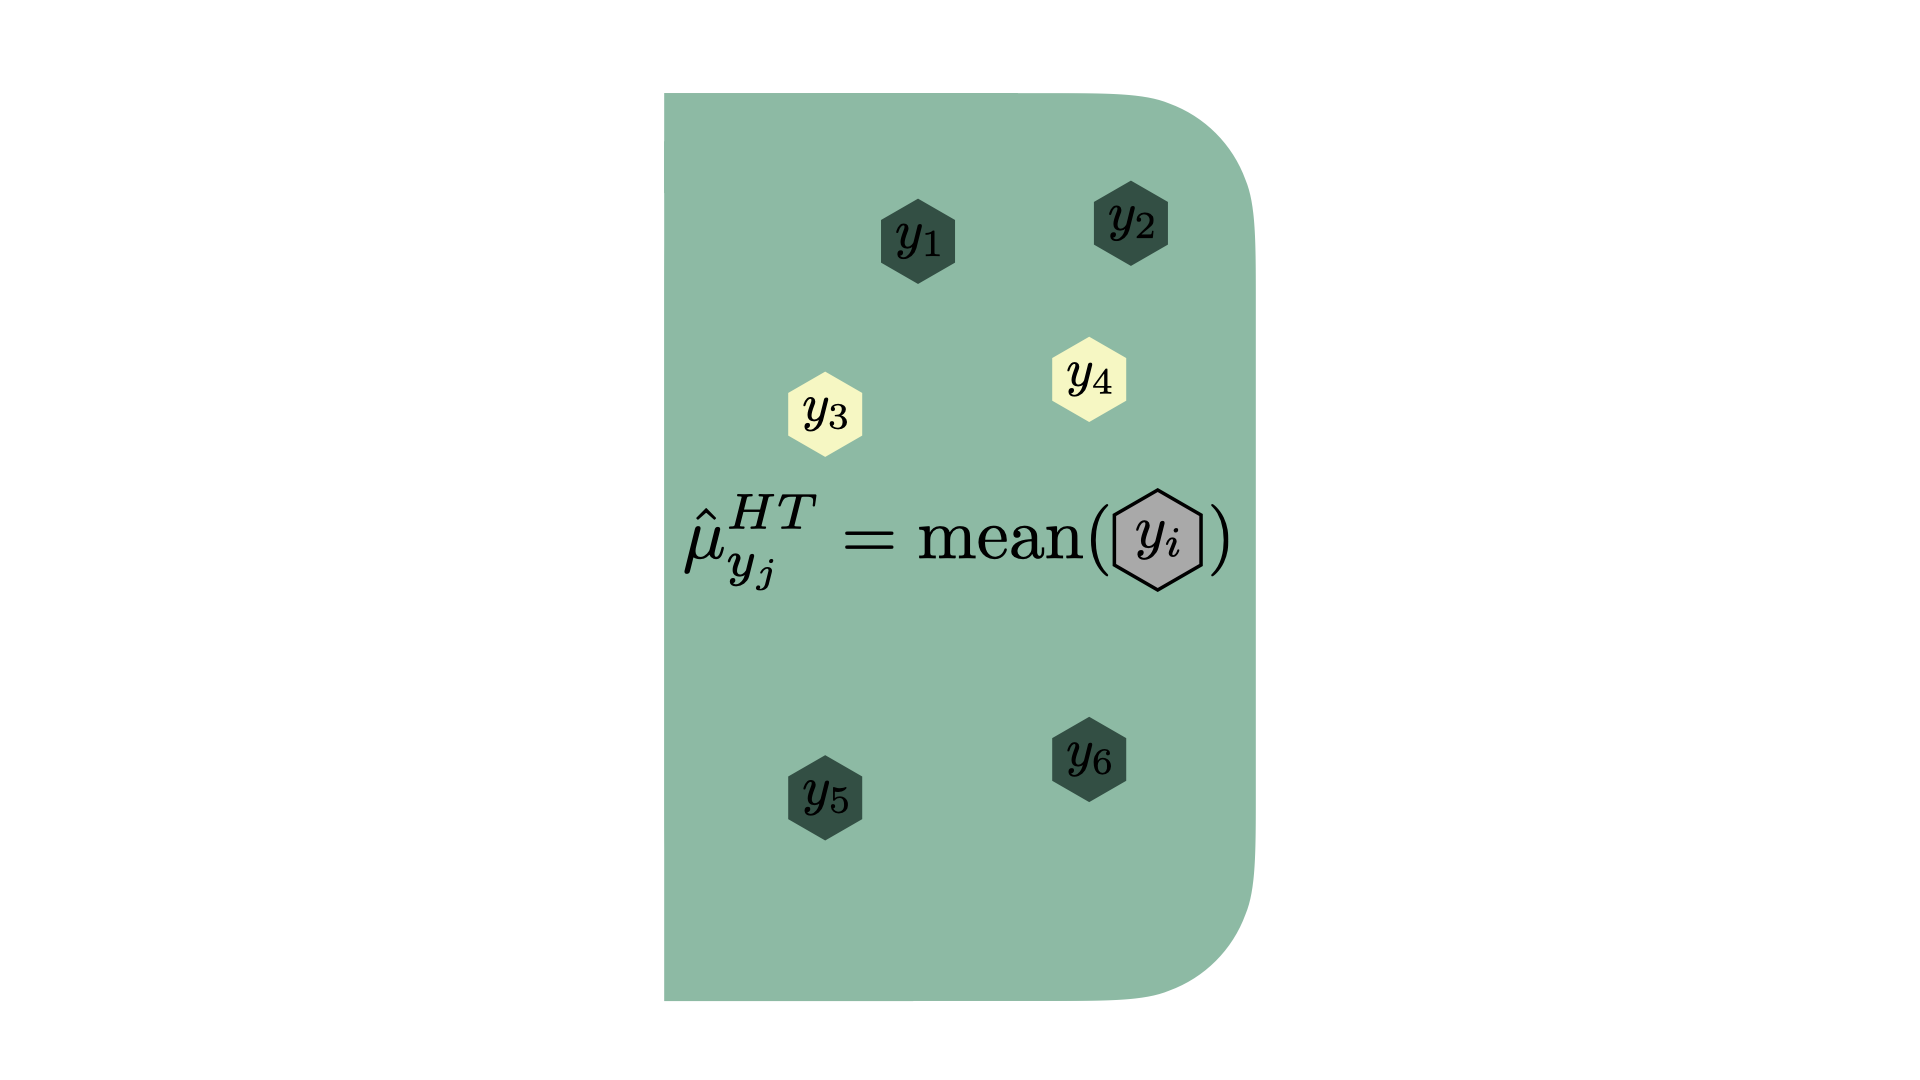
\includegraphics[width=1\linewidth]{figure/mean-diagram} 

}

\caption[The mean as a direct estimator]{The mean as a direct estimator in the seafoam green eco-subsection. This estimator only relies on sampled areas (hexagons) within the eco-subsection. This estimator does not take into account whether the sampled areas are forested (green) or non-forested (beige) areas. This estimator does not use a model to produce estimates and hence uses the \textit{y} variable collected by FIA foresters to produce the needed estimate, as shown inside the hexagons.}\label{fig:mean-diagram}
\end{figure}
\begin{figure}

{\centering 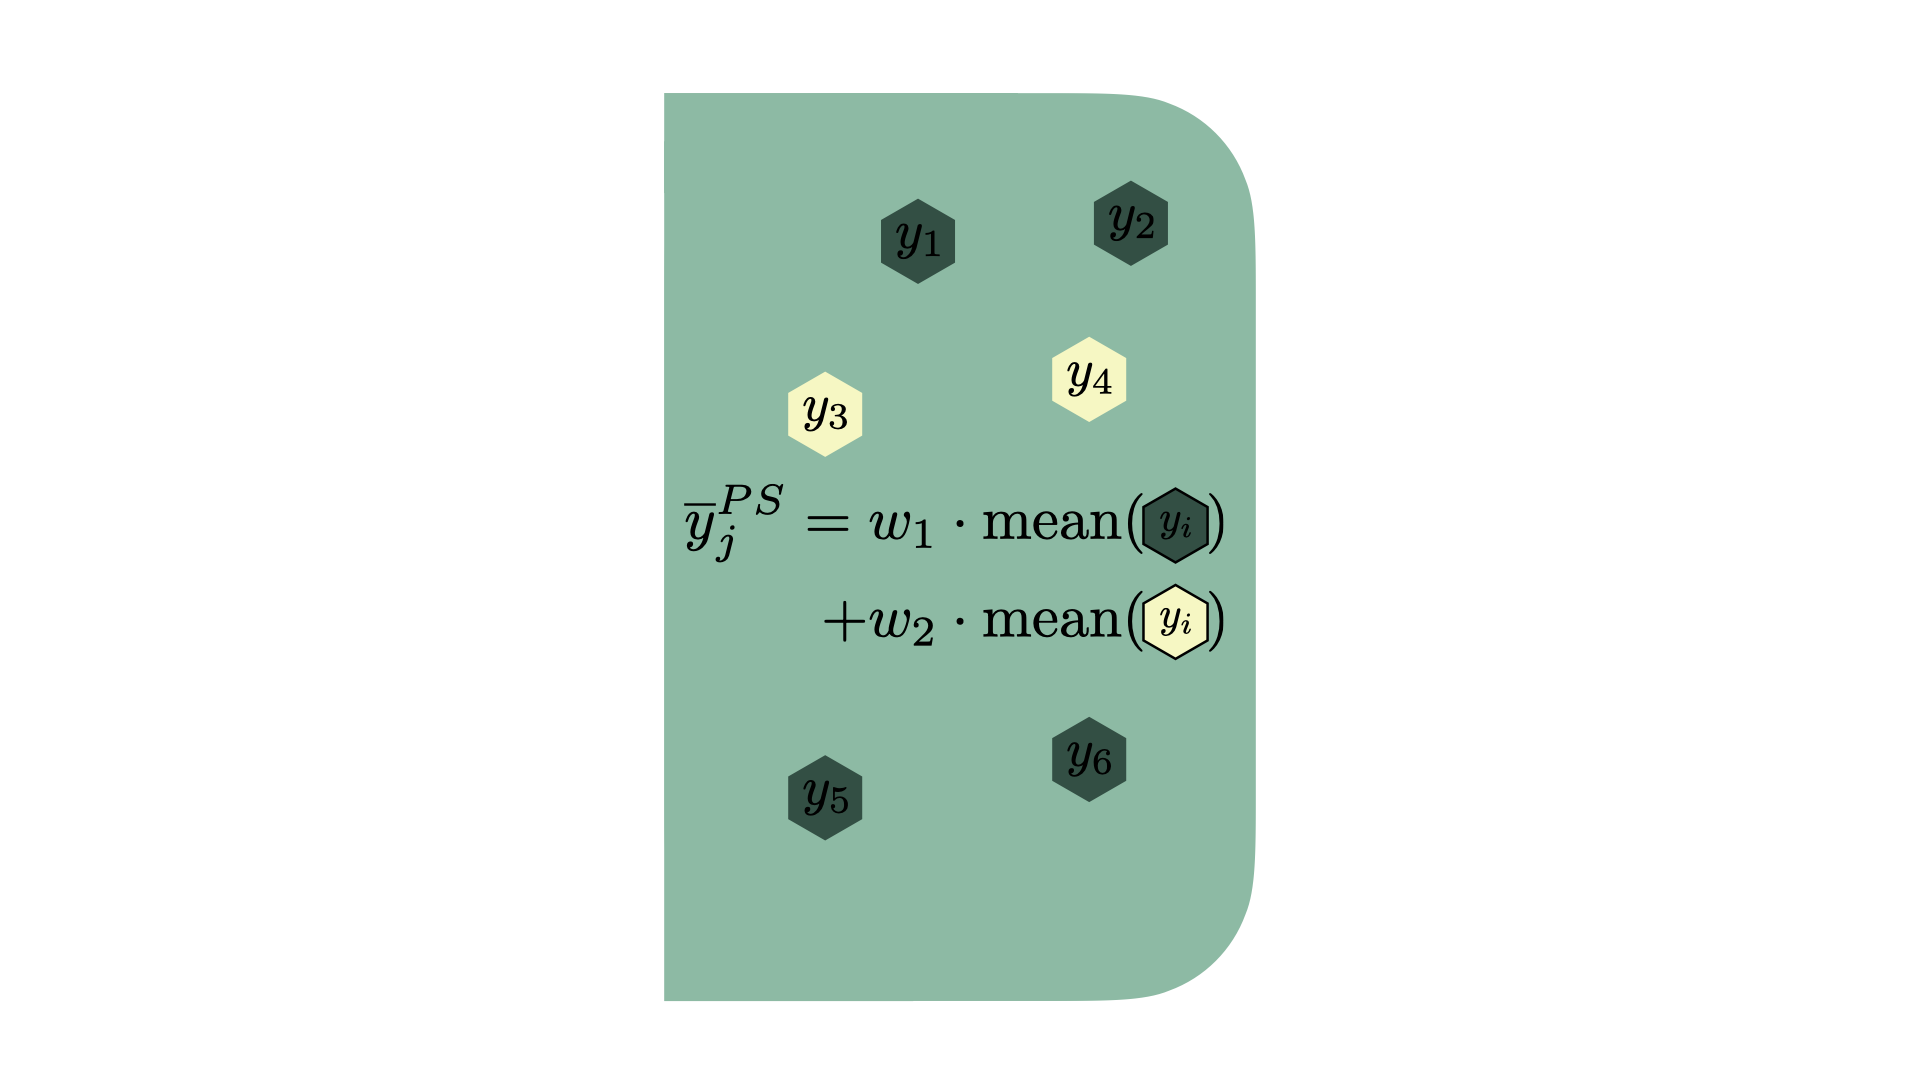
\includegraphics[width=1\linewidth]{figure/ps-diagram} 

}

\caption[The post-stratified direct estimator]{The post-stratified direct estimator in the seafoam green eco-subsection. This estimator only relies on sampled areas (hexagons) within the eco-subsection. This estimator takes into account whether the sampled areas are forested (green) or non-forested (beige) areas. It then weights our estimate based on the true population's proportion of forested area in the eco-subsection. This estimator does not use a model to produce estimates and hence uses the \textit{y} variable collected by FIA foresters to produce the needed estimate, as shown inside the hexagons.}\label{fig:ps-diagram}
\end{figure}
The second kind of estimator, indirect estimators with implicit models, rely on data outside of the area of interest to produce their estimate and can rely on auxiliary data, but implement a model implicitly. With implicit, model-based, indirect estimators we can use information (or ``borrow strength'') from nearby small areas to help improve our estimate (i.e.~reduce variance) in our area of interest through implicit use of a model. These indirect estimators are quite a bit more complicated than direct estimators due to the fact that they borrow strength from the variable of interest across small areas, however, they often significantly reduce variance in estimates due to the added information from other sub-populations. According to Rao (2014), while indirect estimators with implicit models reduce variance, they are often design biased due to the inability to specify between-area variation. This is a large cost of implementing implicit, model-based, indirect estimators. Further, these estimators do not reduce variance as significantly as explicit model-based estimators. Thus, we will not implement indirect estimators with implicit models in this thesis.

Finally, explicit model-based estimators are those which both borrow strength from other small areas, use auxiliary information, and explicitly use a model to compute the estimate of interest. These estimators are still within the family of indirect estimators. However they make explicit use of a model. Similarly to the indirect estimators with implicit models discussed previously, these models can further reduce the variance of our estimates because they allow for more information to be used in the estimate. We can further categorize these explicit model-based estimators into two classes: unit-level and area-level models. Unit-level models consider information at the level of which the data was collected. Area-level models consider information that has been aggregated to the level of a small area before the model is fit to the data. Commonly, the empirical best linear unbiased prediction model (EBLUP) is used in small area estimation as the model-based estimator of choice. This is because both the area- and unit-level EBLUP models reduce variance further than direct and indirect estimators with implicit models, and they are design unbiased given the modeling assumptions are met. This thesis primarily investigates the usefulness of the hierarchical Bayesian unit-level model (HBU) and hierarchical Bayesian area-level model (HBA). We can visualize HBU and HBA estimators to give a better sense of the differences between the two.
\begin{figure}

{\centering 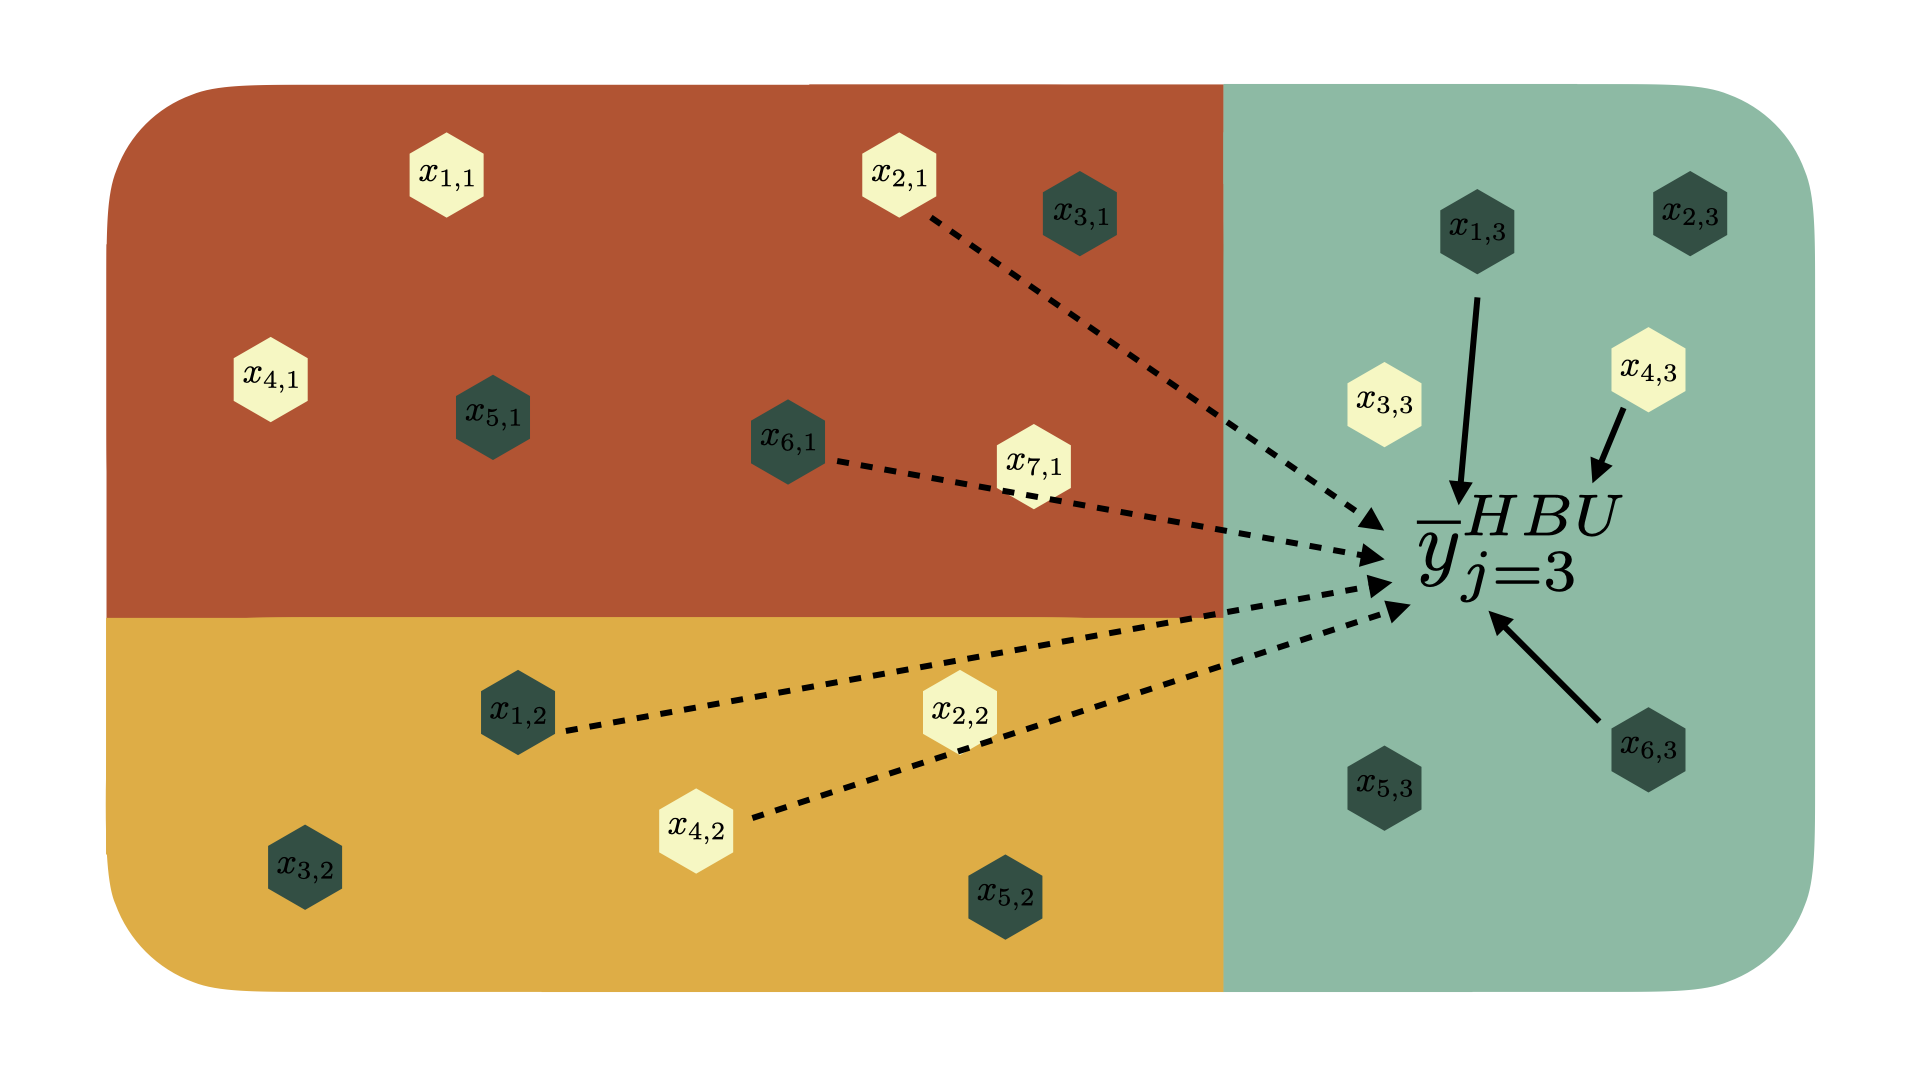
\includegraphics[width=1\linewidth]{figure/hbu-diagram} 

}

\caption[The unit-level hierarchical Bayesian model]{The unit-level hierarchical Bayesian model producing an estimate in our seafoam green eco-subsection. This estimator relies on auxiliary information from all eco-subsections within a given eco-province to produce estimates as shown by the arrows. Notably, more information is used in the eco-subsection of interest to produce the estimate, denoted by the solid arrows. The dashed arrows tell us that less information is being used from outside eco-subsections. This estimator also produces estimates based on remotely sensed data, as denoted by the \textit{x} variables in each hexagon. This estimator uses information at the unit-level, meaning that it produces estimates from the plot level of granularity.}\label{fig:hbu-diagram}
\end{figure}
\begin{figure}

{\centering 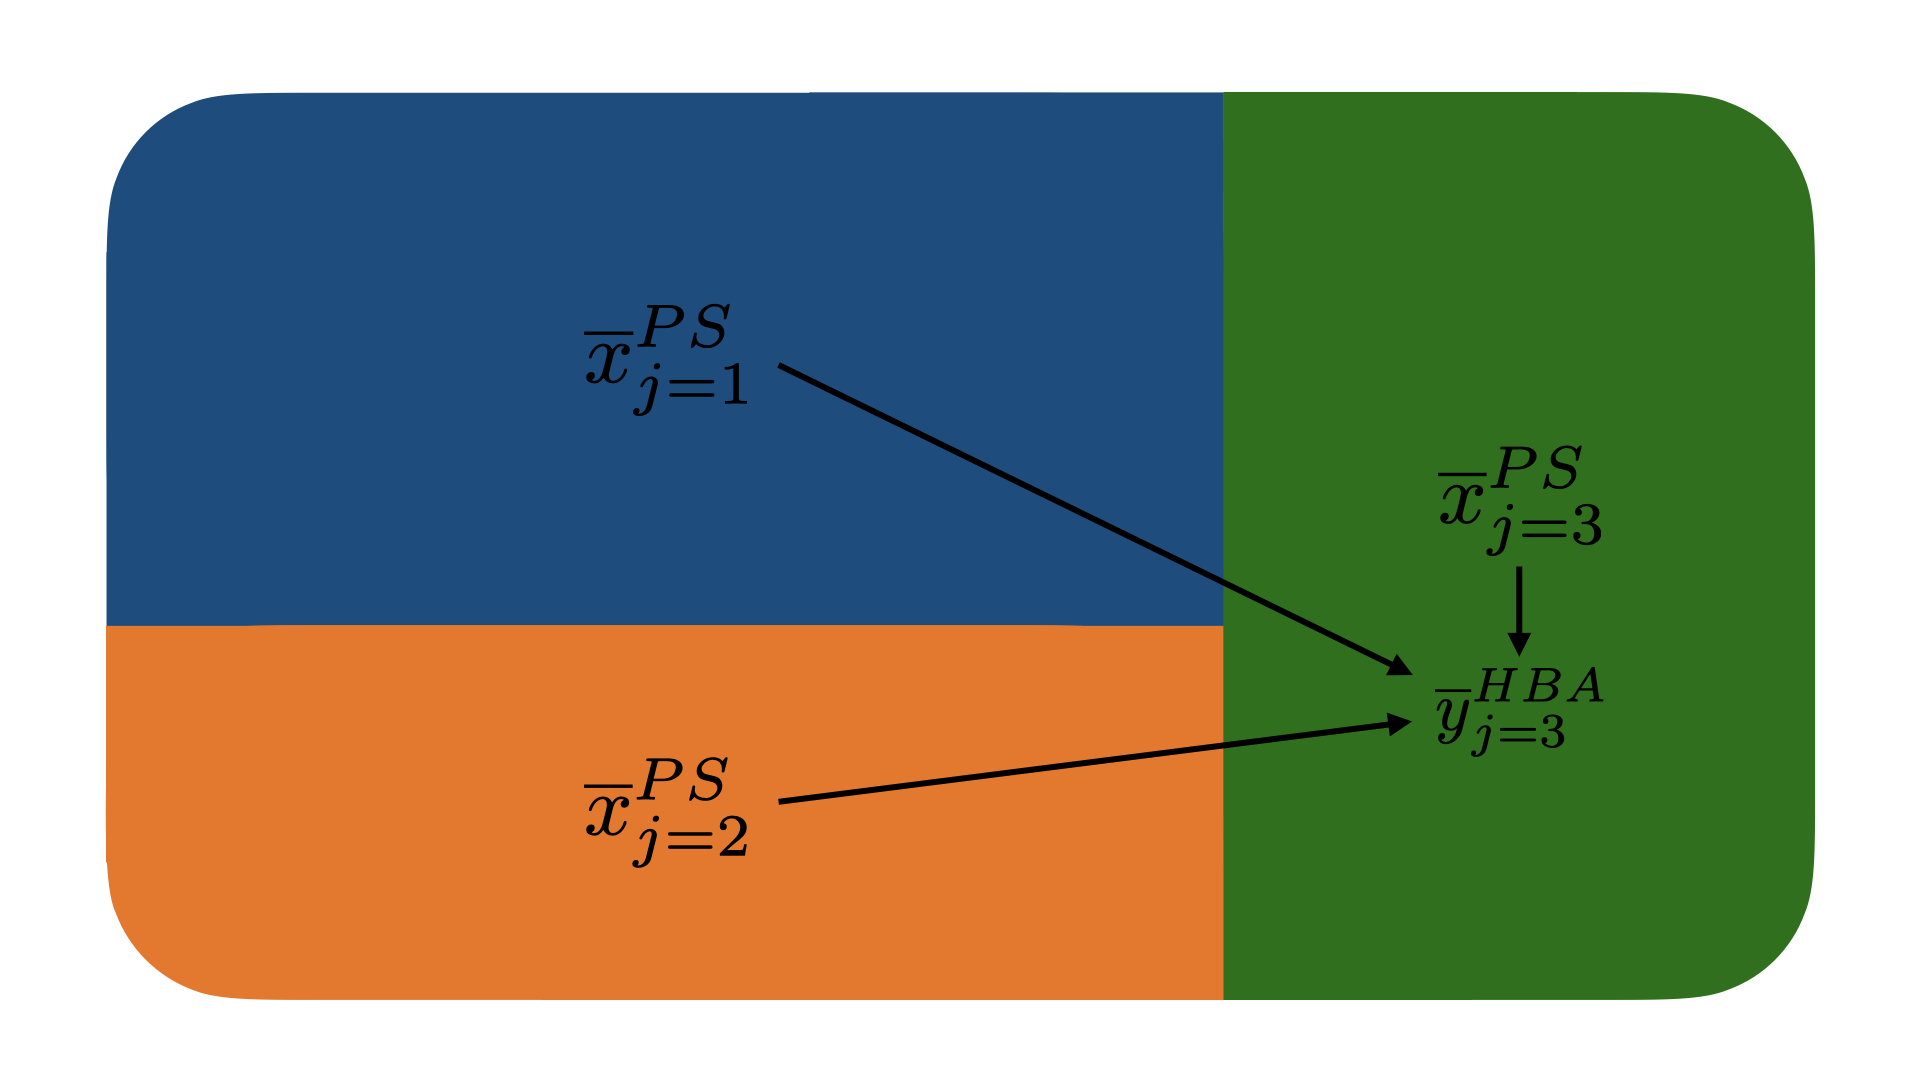
\includegraphics[width=1\linewidth]{figure/hba-diagram} 

}

\caption[The area-level hierarchical Bayesian model]{The area-level hierarchical Bayesian model producing an estimate in our seafoam green eco-subsection. This estimator relies on auxiliary information from all eco-subsections within a given eco-province to produce estimates as shown by the arrows. Notably, more information is used in the eco-subsection of interest to produce the estimate, denoted by the solid arrows. The dashed arrows tell us that less information is being used from outside eco-subsections. This estimator also produces estimates based on remotely sensed data, as denoted by the \textit{x} variables in each hexagon. This estimator uses information at the area-level, meaning that it produces estimates based on the post-stratified estimate in each eco-subsection.}\label{fig:hba-diagram}
\end{figure}
It is important to note that while Figures \ref{fig:hbu-diagram} and \ref{fig:hba-diagram} describe the hierarchical Bayesian estimators, the diagrams would be the same for the unit- and area-level EBLUP estimators. This is due to the fact that the EBLUP estimators assume a frequentist mixed model rather than a Bayesian one. These estimators are of course different, we just do not explicitly show how the magnitude of strength borrowed is decided in Figures \ref{fig:hbu-diagram} and \ref{fig:hba-diagram}.

We can see that both the hierarchical Bayesian unit- and area-level models borrow strength from surrounding areas and explicitly model the \(y\) variable outcome as a function of remotely sensed \(x\) variable(s). The notable difference between the two models is that the hierarchical Bayesian unit-level models borrows strength from the unit-level data while the area-level model borrows strength from data aggregated by the post-stratified direct estimator.

Explicit model-based estimation has been increasing in popularity in the realm of applications to the FIA and forestry data in general. As the FIA requires a reduction in variance for their estimates of increasingly smaller areas, it becomes inevitable that borrowing strength from surrounding areas, the use of auxiliary data, and the explicit use of a model is needed to maintain a satisfactory amount of variance. Commonly, frequentist model-based estimators are used for model-based small area estimation, such as the EBLUP estimator. Models such as the EBLUP have some very nice properties. Most notably, they are ``unbiased'' if the assumed model is correct. To understand what it means to have an ``unbiased'' estimator, we must first define bias of some estimator \(\hat\mu_{y_j}\) of a parameter \(\mu_{y_j}\):
\begin{align}
\text{Bias}(\hat\mu_{y_j}) = E[\hat\mu_{y_j}] - \mu_{y_j}
\end{align}
It intuitively follows that if the modeling assumptions are met and our estimator \(\hat\mu_{y_j}\) is unbiased that we will have the following property:
\begin{align}
\text{Bias}(\hat\mu_{y_j}) = E[\hat\mu_{y_j}] - \mu_{y_j} = 0
\end{align}
That is, the expected value of the estimator, \(\hat\mu_{y_j}\), is in fact the true value of the forest attribute of interest. It is clear as to why this is a trait we would want in our model and to why it is so commonly used, however, what is not clear is the cost of this trait. By only focusing on reducing the bias in our estimates, we must ignore the second piece of the mean squared error, the variance. While it is important for bias to be low, we can often reduce our mean squared error by a large amount by increasing bias slightly, as bias and variance are inversely related. We can see by the representation of the mean squared error (MSE) as the sum of the variance and squared bias of our estimator:
\begin{align}
\text{MSE}(\hat\mu_{y_j}) = \text{Var}(\hat\mu_{y_j}) + \text{Bias}(\hat\mu_{y_j},~ \mu_{y_j})^2
\end{align}
This thesis explores this trade-off between bias and variance in depth. We implement hierarchical Bayesian unit- and area-level models which allow for the estimates to be slightly biased while reducing variance. Throughout this thesis, we compare these techniques to small area estimations methods such as the EBLUP and the post-stratified direct estimator. By applying these models on four response variables across the entire Interior West at the eco-subsection level, we can add a great deal of understanding to the usefulness of hierarchical Bayesian models in a small area estimation context, especially when considering its usefulness to the FIA and other forestry organizations. We only have been able to source one paper which uses hierarchical Bayesian modeling for small area estimation with a forestry application, and they only consider the area-level model with a particular response variable in particular forest (Ver Planck, Finley, \& Huff, 2017). This thesis thus adds significantly to our understanding of the usefulness of hierarchical Bayesian small area estimation in a forestry setting due to the introduction of the unit-level model, the vast number of response variables studied, and the vast range of area where we test the usefulness of this model.

\hypertarget{overview}{%
\chapter{Overview}\label{overview}}

\hypertarget{data}{%
\chapter{Data}\label{data}}

\hypertarget{the-forest-inventory-analysis-program}{%
\section{The Forest Inventory \& Analysis Program}\label{the-forest-inventory-analysis-program}}

The FIA is a program within the United States Forest Service which aims to collect information and data in order to assess the country's forests. The FIA has been continuously operating since 1930 and their official mission is to ``make and keep current a comprehensive inventory and analysis of the present and prospective conditions of and requirements for the renewable resources of the forest and rangelands of the US'' (FIA, 2020).

The FIA collects data all throughout the United States by completing a survey each year of many plots of land. The units measured by the FIA and their ground crews are approximately 30 meter by 30 meter hexagonal units. Due to the vast size of the United States and immense amount of forested land, it would be nearly impossible for the FIA to attain population data for the country, so they use sampling instead. The FIA samples from the population of 30 meter by 30 meter hexagonal units by using a geographically-based systematic sampling design (McConville, Moisen, \& Frescino, 2020). The FIA chooses these samples by first overlaying a hexagonal grid over the United States where each hexagon contains approximately 6000 acres of land. Then, they fill these hexagons with much smaller hexagons and randomly sample from the population of small hexagons. Then, ground crews go to these sampled small hexagons and collect variables such as basal area, trees per acre, etc. Along with this hand-collected data from FIA ground crews, the FIA also uses remotely sensed data to gain more information about the areas which they collect data. For example, the \texttt{nlcd11} variable, which measures total percent tree canopy cover of a plot, is collected via remote sensing by the Multi-Resolution Land Characteristics Consortium (Homer, 2015). Throughout the duration of the thesis, we will be working to predict ground-collected data with remotely sensed variables, such as \texttt{nlcd11}. Having remotely sensed variables like \texttt{nlcd11} is useful to us and the FIA because if our models can predict ground-collected variables well, the FIA can collect less data and have a larger effective sample size.

\hypertarget{the-interior-west}{%
\section{The Interior West}\label{the-interior-west}}

While the FIA collects data in all regions of the United States, the analyses done in this thesis uses data from the Interior West Forest Inventory and Analysis Unit (IW-FIA). Data from this unit will henceforth be referred to as data from ``the Interior West''. The Interior West is defined as a broad region of the United States, covering the states of Arizona, Colorado, Idaho, Montana, Nevada, New Mexico, Utah, and Wyoming. For reference we have provided the Interior West colored green on a map of the continental United States:
\begin{figure}

{\centering 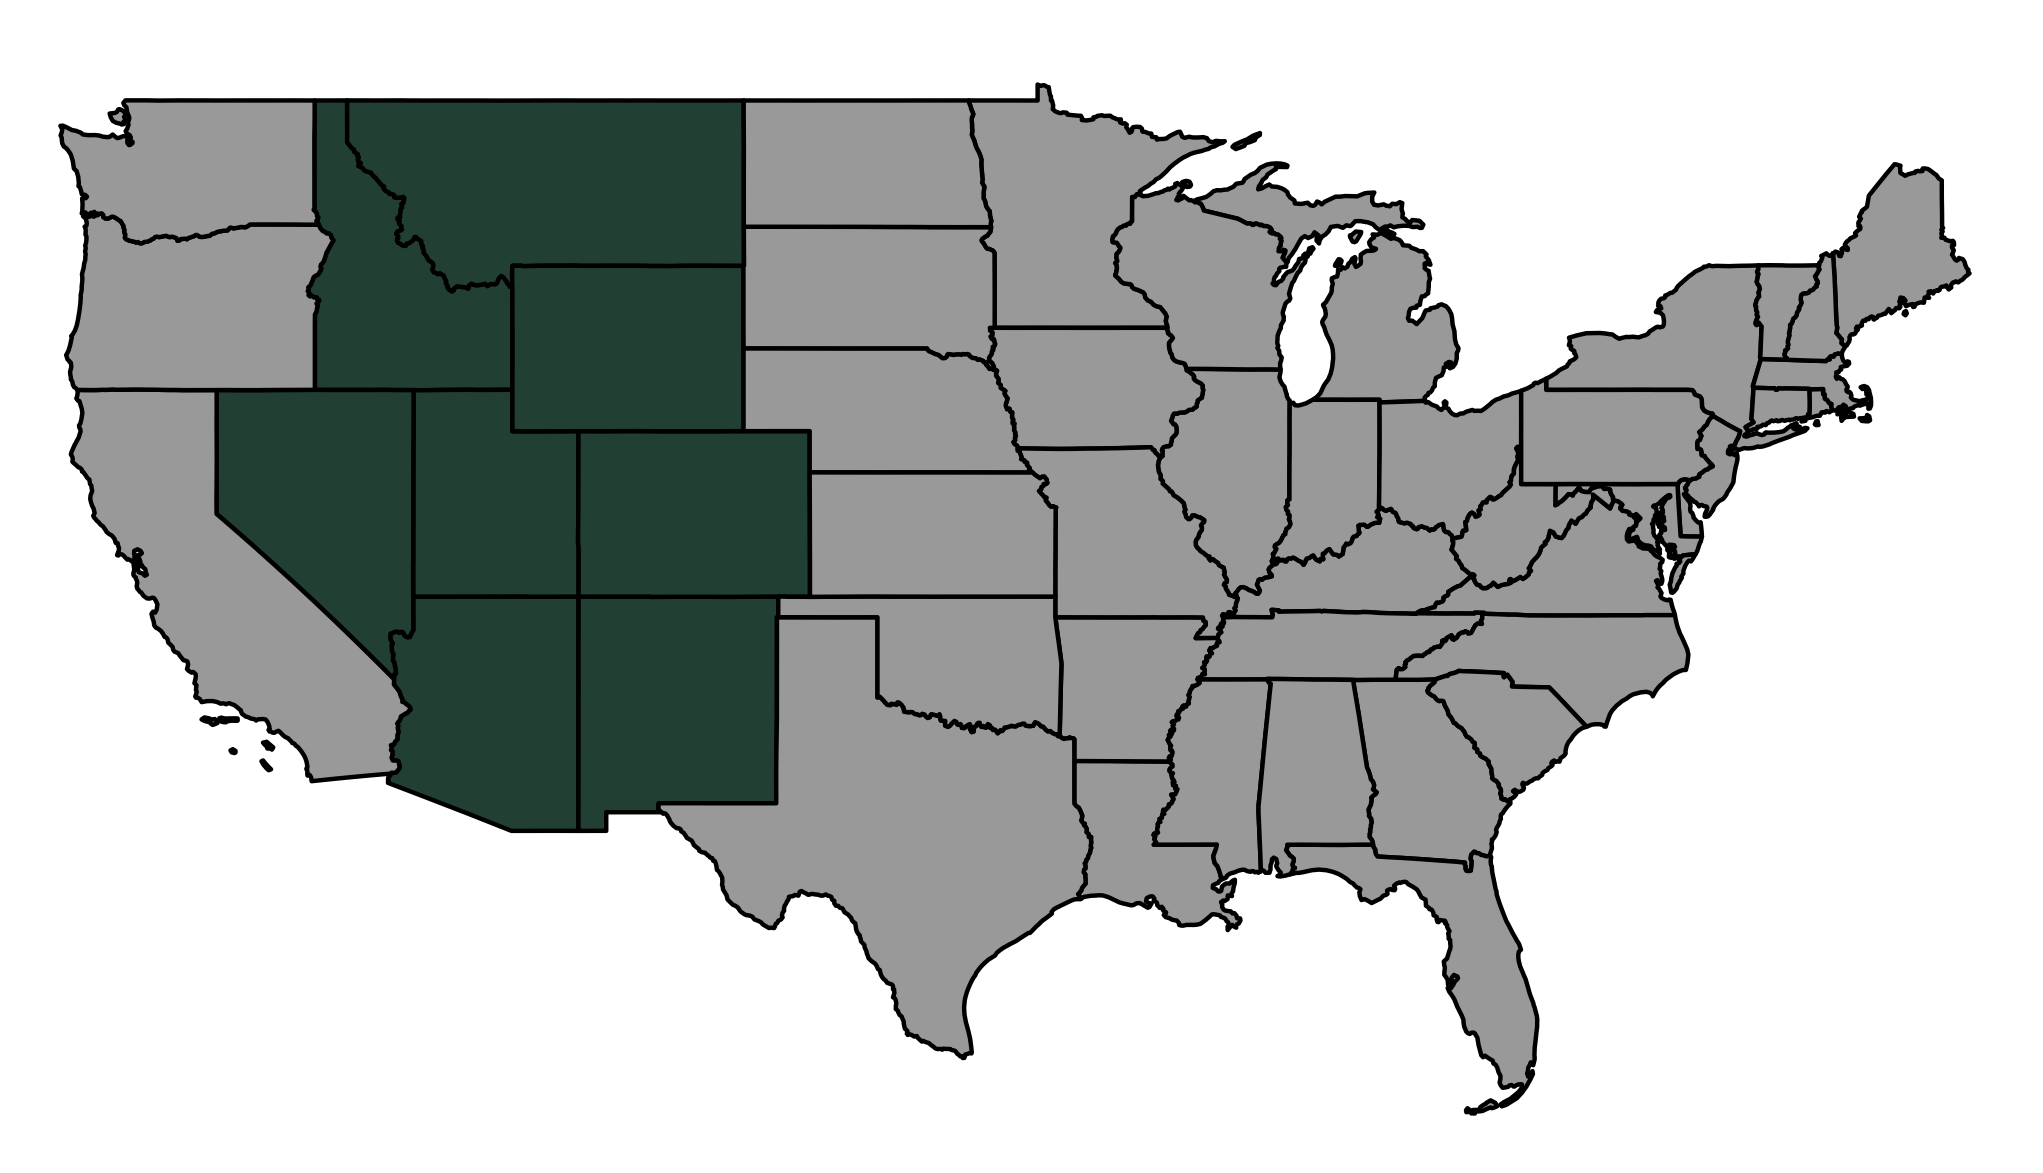
\includegraphics[width=1\linewidth]{figure/interior-west-on-usa} 

}

\caption{The Interior West region of the United States}\label{fig:unnamed-chunk-3}
\end{figure}
The IW-FIA collects annual inventories of the Interior West, with the goal of covering 10\% of the region each year, so every decade the IW-FIA should have measurement of 100\% of each Interior West state's forests.

The Interior West region itself contains the states which encompass the Rocky Mountains along with some other smaller mountain ranges. The Interior West contains 855,767 square miles of land which has an extremely diverse landscape ranging from the high mountain peaks of the Rockies to flat desert plains in Nevada and other Interior West states. Along with desert and mountains, the Interior West also includes parts of the Great Plains. Throughout this diverse landscape, there is a similarly diverse range of forested areas. The forested areas range from areas that are humid and temperate to areas like the Northern Rocky Mountain Forest which is dry and considered a temperate desert.

\hypertarget{our-data-specifics}{%
\section{Our Data: Specifics}\label{our-data-specifics}}

The data used in this thesis was collected by the FIA in the span of 10 years from 2007 to 2017. While this data was collected over this 10 year period, the analyses done throughout this thesis are under the assumption that this is a ``snapshot'' of the Interior West at some moment in time. Thus we do not consider any temporal features of this dataset, however the inventory year information is available to us. The data we have is plot-level (sometimes referred to as ``unit-level'') data for the Interior West region of the United States, where the data for each plot consists of ground data collected by FIA and remotely sensed data.

The dataframe used in this thesis is a joined dataframe derived from two FIA datasets of the Interior West, \texttt{spatial} and \texttt{response}. The \texttt{spatial} dataframe contains 89444 observations and 70 variables, most notably our remotely sensed predictor variable (\texttt{nlcd11}), location information, and eco-subsection. The \texttt{nlcd11} variable was collected by the Multi-Resolution Land Characteristics Consortium (Homer, 2015). This variable measures percent tree canopy cover in a given plot.

The \texttt{response} dataframe contains 86085 observations and 67 variables, most notably four response variables collected by FIA crew members (\texttt{BALIVE\_TPA}, \texttt{CNTLIVE\_TPA}, \texttt{BIOLIVE\_TPA}, and \texttt{VOLNLIVE\_TPA}), location information, and eco-subsection. The response variables noted above measure basal area, tree count, biomass, and volume, respectively. We join these dataframes by their unique plot number, and subset the number of variables significantly to 19 variables which contain plot information, longitude \& latitude, elevation, predictor variables, response variables, eco-subsection, eco-section, and eco-province. The resulting joined dataframe has 86085 rows as these are the rows which share the same plots between the \texttt{response} and \texttt{spatial} dataframes. We can see the first few rows of the dataframe with relevant columns selected and values rounded to the second decimal place:
\begin{longtable}[t]{rrrrrl}
\caption[Relevant Glimpse of Data]{\label{tab:unnamed-chunk-4}Relevant Glimpse of Data}\\
\toprule
Plot & Latitude & Longitude & nlcd11 & BIOLIVE\_TPA & subsection\\
\midrule
83574 & -109.71 & 32.85 & 21 & 0.00 & 321Af\\
84904 & -109.88 & 32.99 & 0 & 0.00 & 321Af\\
83021 & -109.88 & 32.81 & 0 & 0.00 & 321Aj\\
82635 & -109.89 & 32.65 & 26 & 14.74 & 321Am\\
90381 & -109.83 & 32.62 & 41 & 31.50 & 321Am\\
\addlinespace
81801 & -109.79 & 32.35 & 0 & 0.00 & 321Aj\\
\bottomrule
\end{longtable}
While the data covers the Interior West as a whole, we have very granular information, as each row represents a plot sampled by the FIA. The data also includes variables that subset the Interior West into provinces which contain eco-sections, and these eco-sections contain eco-subsections. In our data, on average, each eco-section contains approximately 7.06 eco-subsections, and each province contains an average of 4.86 eco-sections. So, an average province then contains just over 34 eco-subsections. We can take a look at the Northern Rocky Forest province, colored by eco-section, with lines dividing each eco-subsection to see this structure in action:
\begin{figure}

{\centering 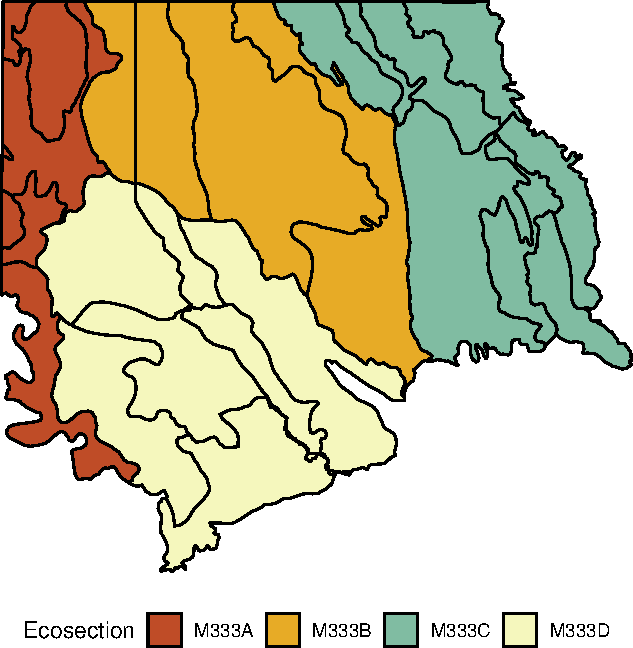
\includegraphics{thesis_files/figure-latex/northern-rocky-1} 

}

\caption{The Northern Rocky Forest colored by eco-section}\label{fig:northern-rocky}
\end{figure}
The data we have covers a total of 14 provinces, 68 eco-sections, and 480 eco-subsections. The hierarchical structure of the data and nested nature of the eco-subsections within eco-sections within eco-provinces lends itself to be able to create hierarchical models which borrow strength from surrounding areas.

While this data contains a multitude of variables, the analyses done in this thesis focus on four key response variables and one explanatory variable. The response variables used are basal area (square-foot), trees per acre, above-ground biomass (lbs), and net volume (\(\text{ft}^3\)). These variables are coded as \texttt{BALIVE\_TPA}, \texttt{CNTLIVE\_TPA}, \texttt{BIOLIVE\_TPA}, and \texttt{VOLNLIVE\_TPA}, respectively. We can look at the average of these variables across the Interior West region by eco-subsection in the four following maps of the interior west.
\begin{figure}

{\centering 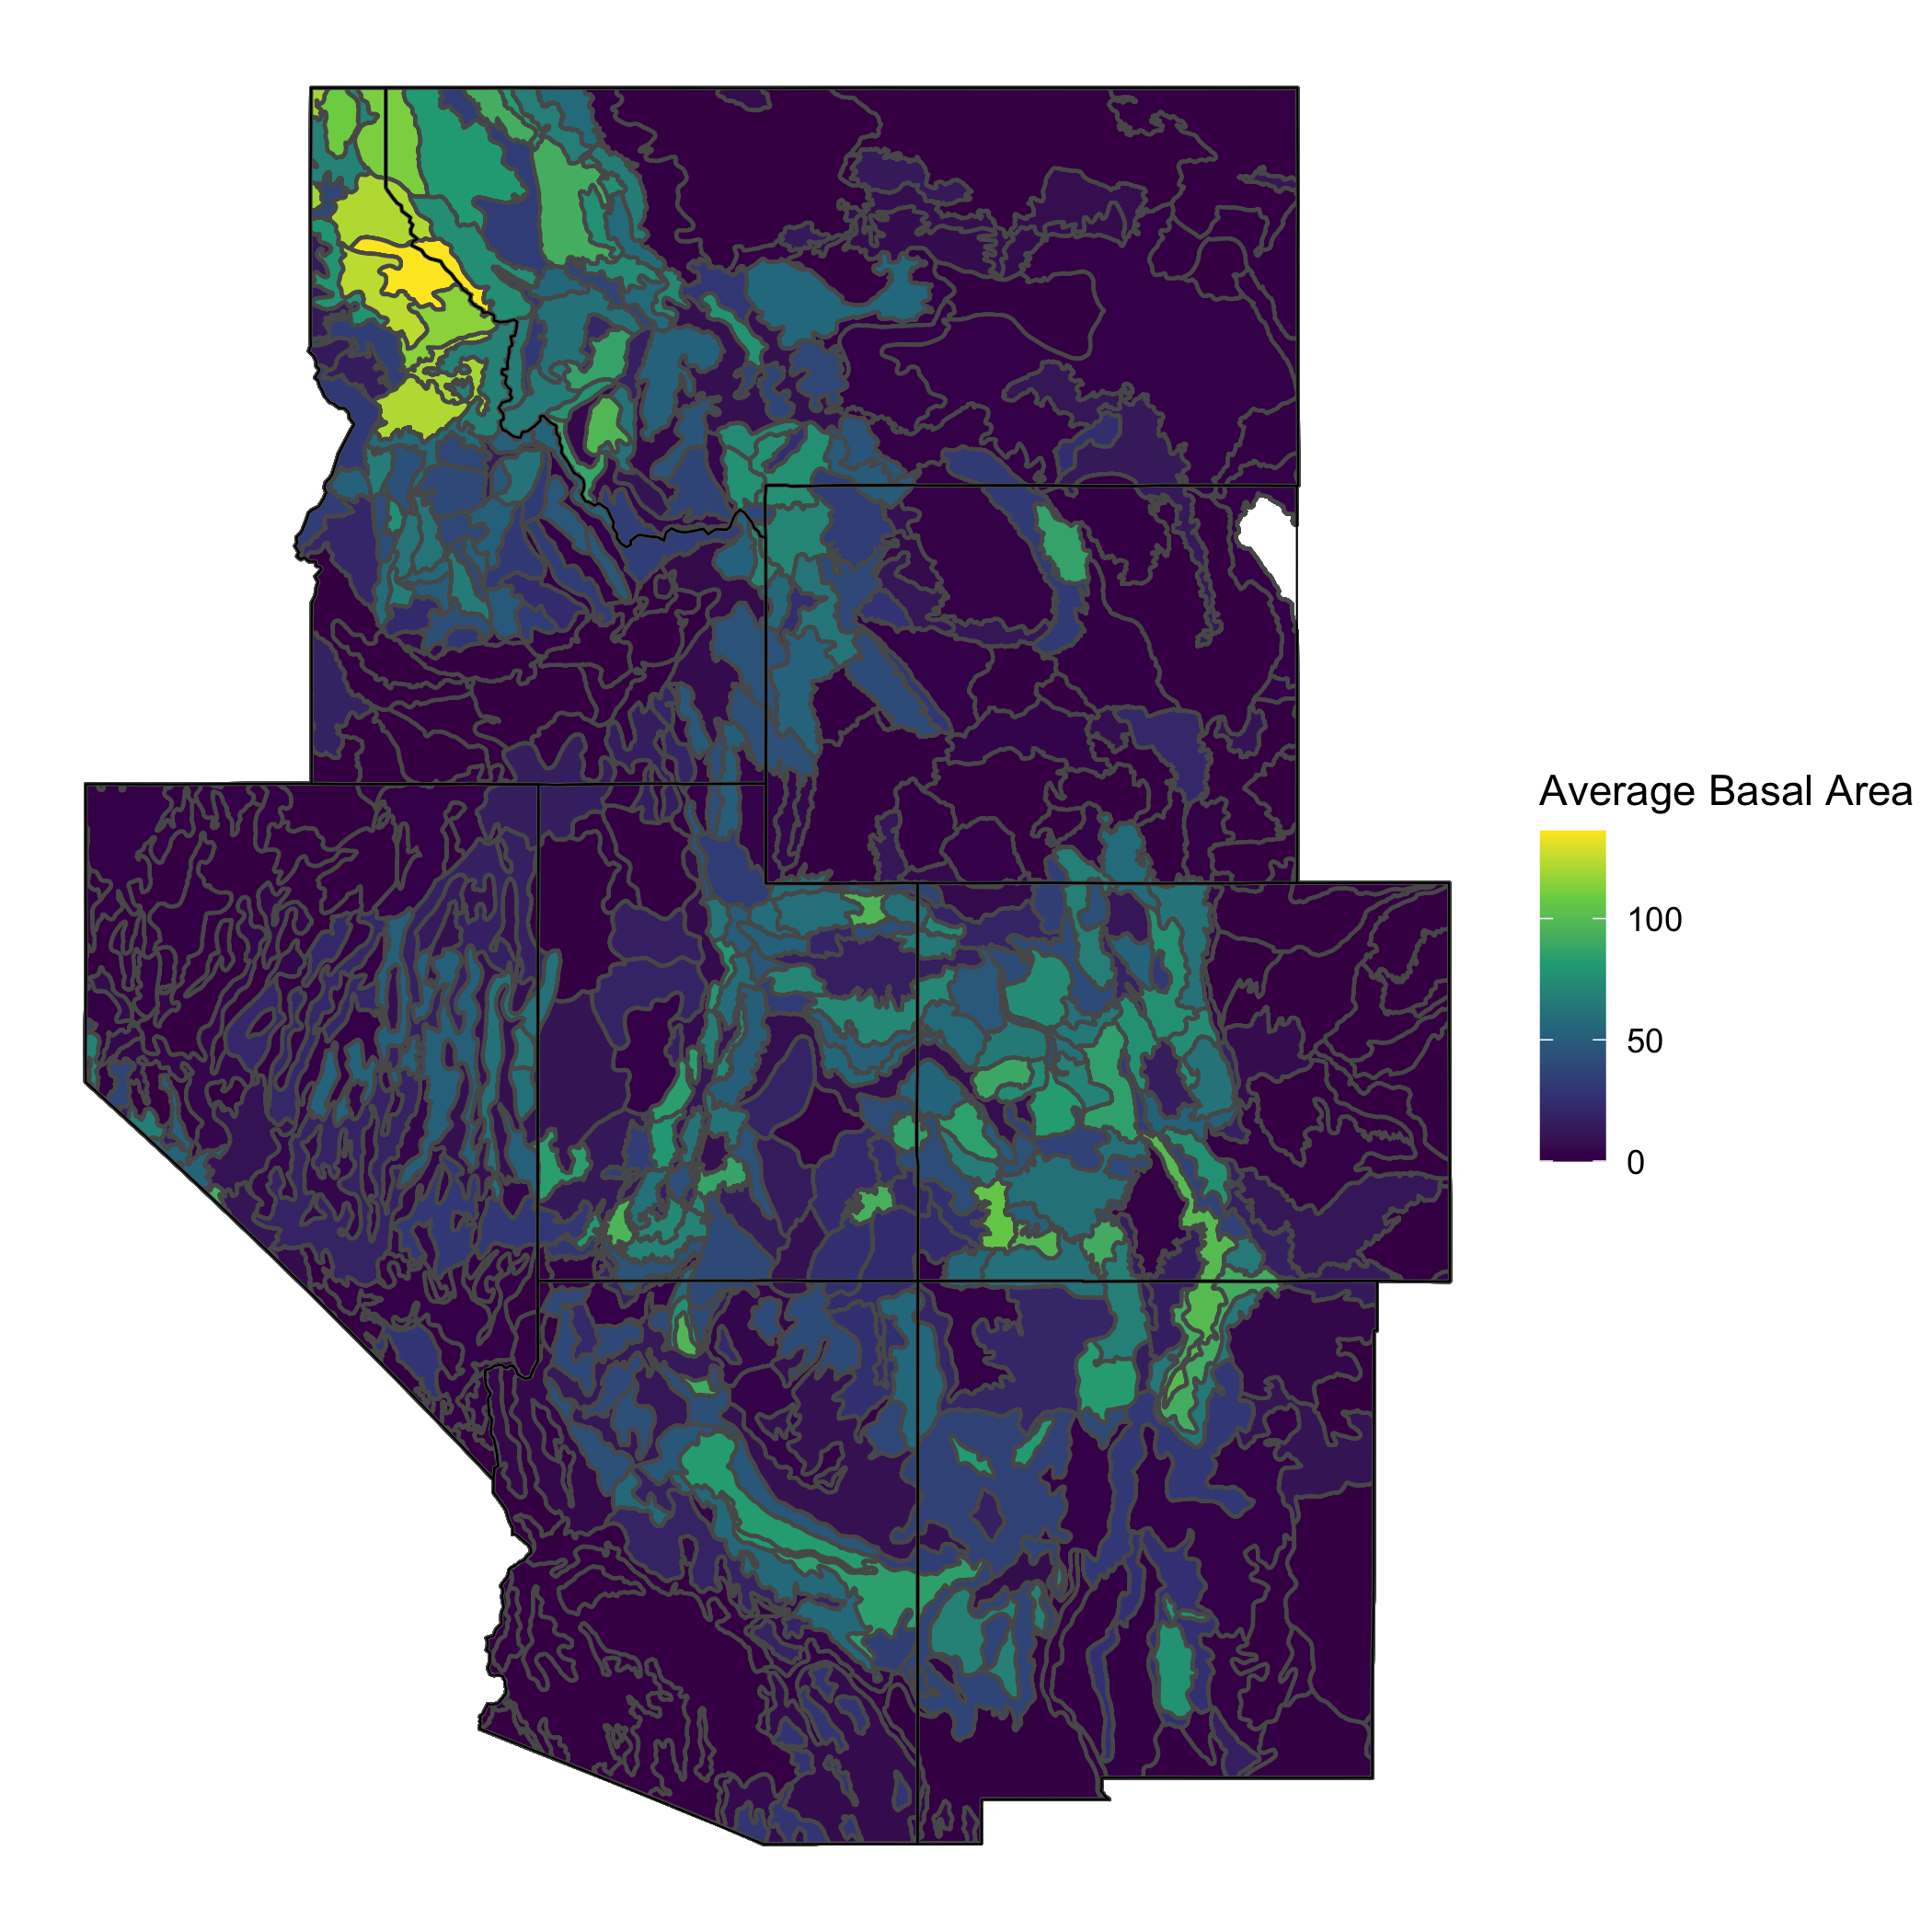
\includegraphics[width=0.65\linewidth]{figure/basal} 

}

\caption{Mean basal area in Interior West eco-subsections}\label{fig:unnamed-chunk-5}
\end{figure}
\begin{figure}

{\centering 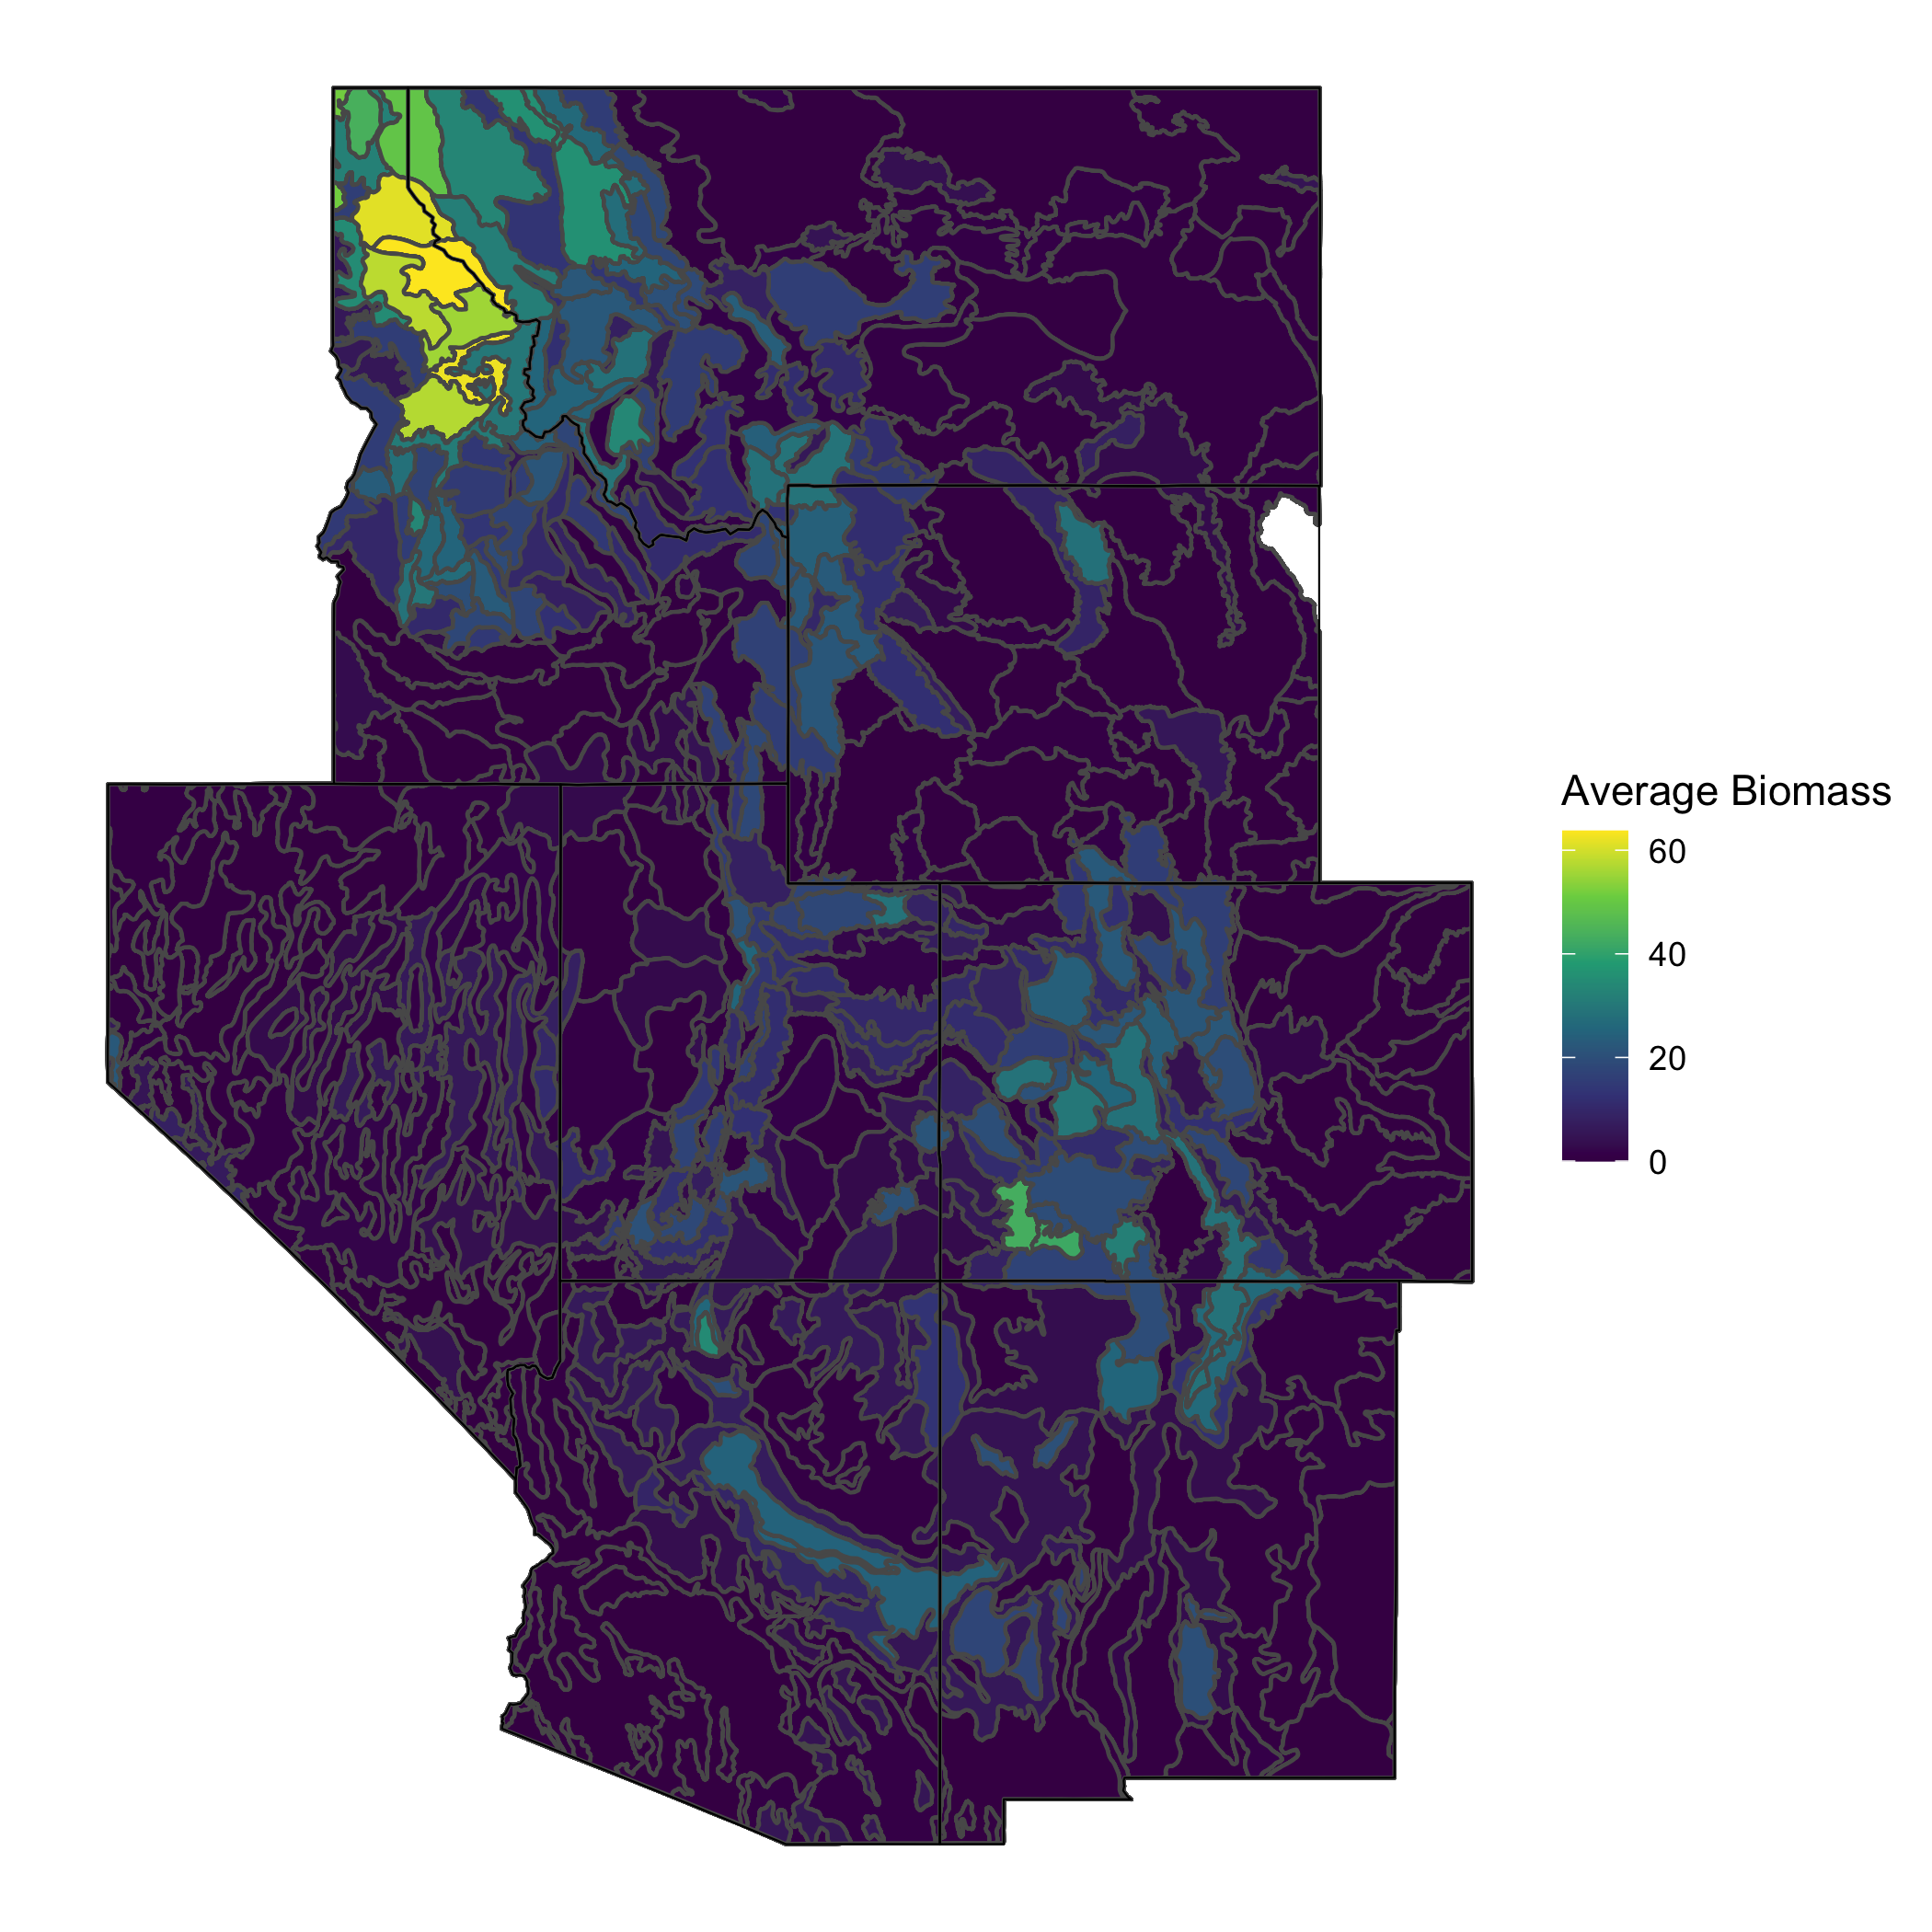
\includegraphics[width=0.65\linewidth]{figure/biomass} 

}

\caption{Mean biomass in Interior West eco-subsections}\label{fig:unnamed-chunk-6}
\end{figure}
\begin{figure}

{\centering 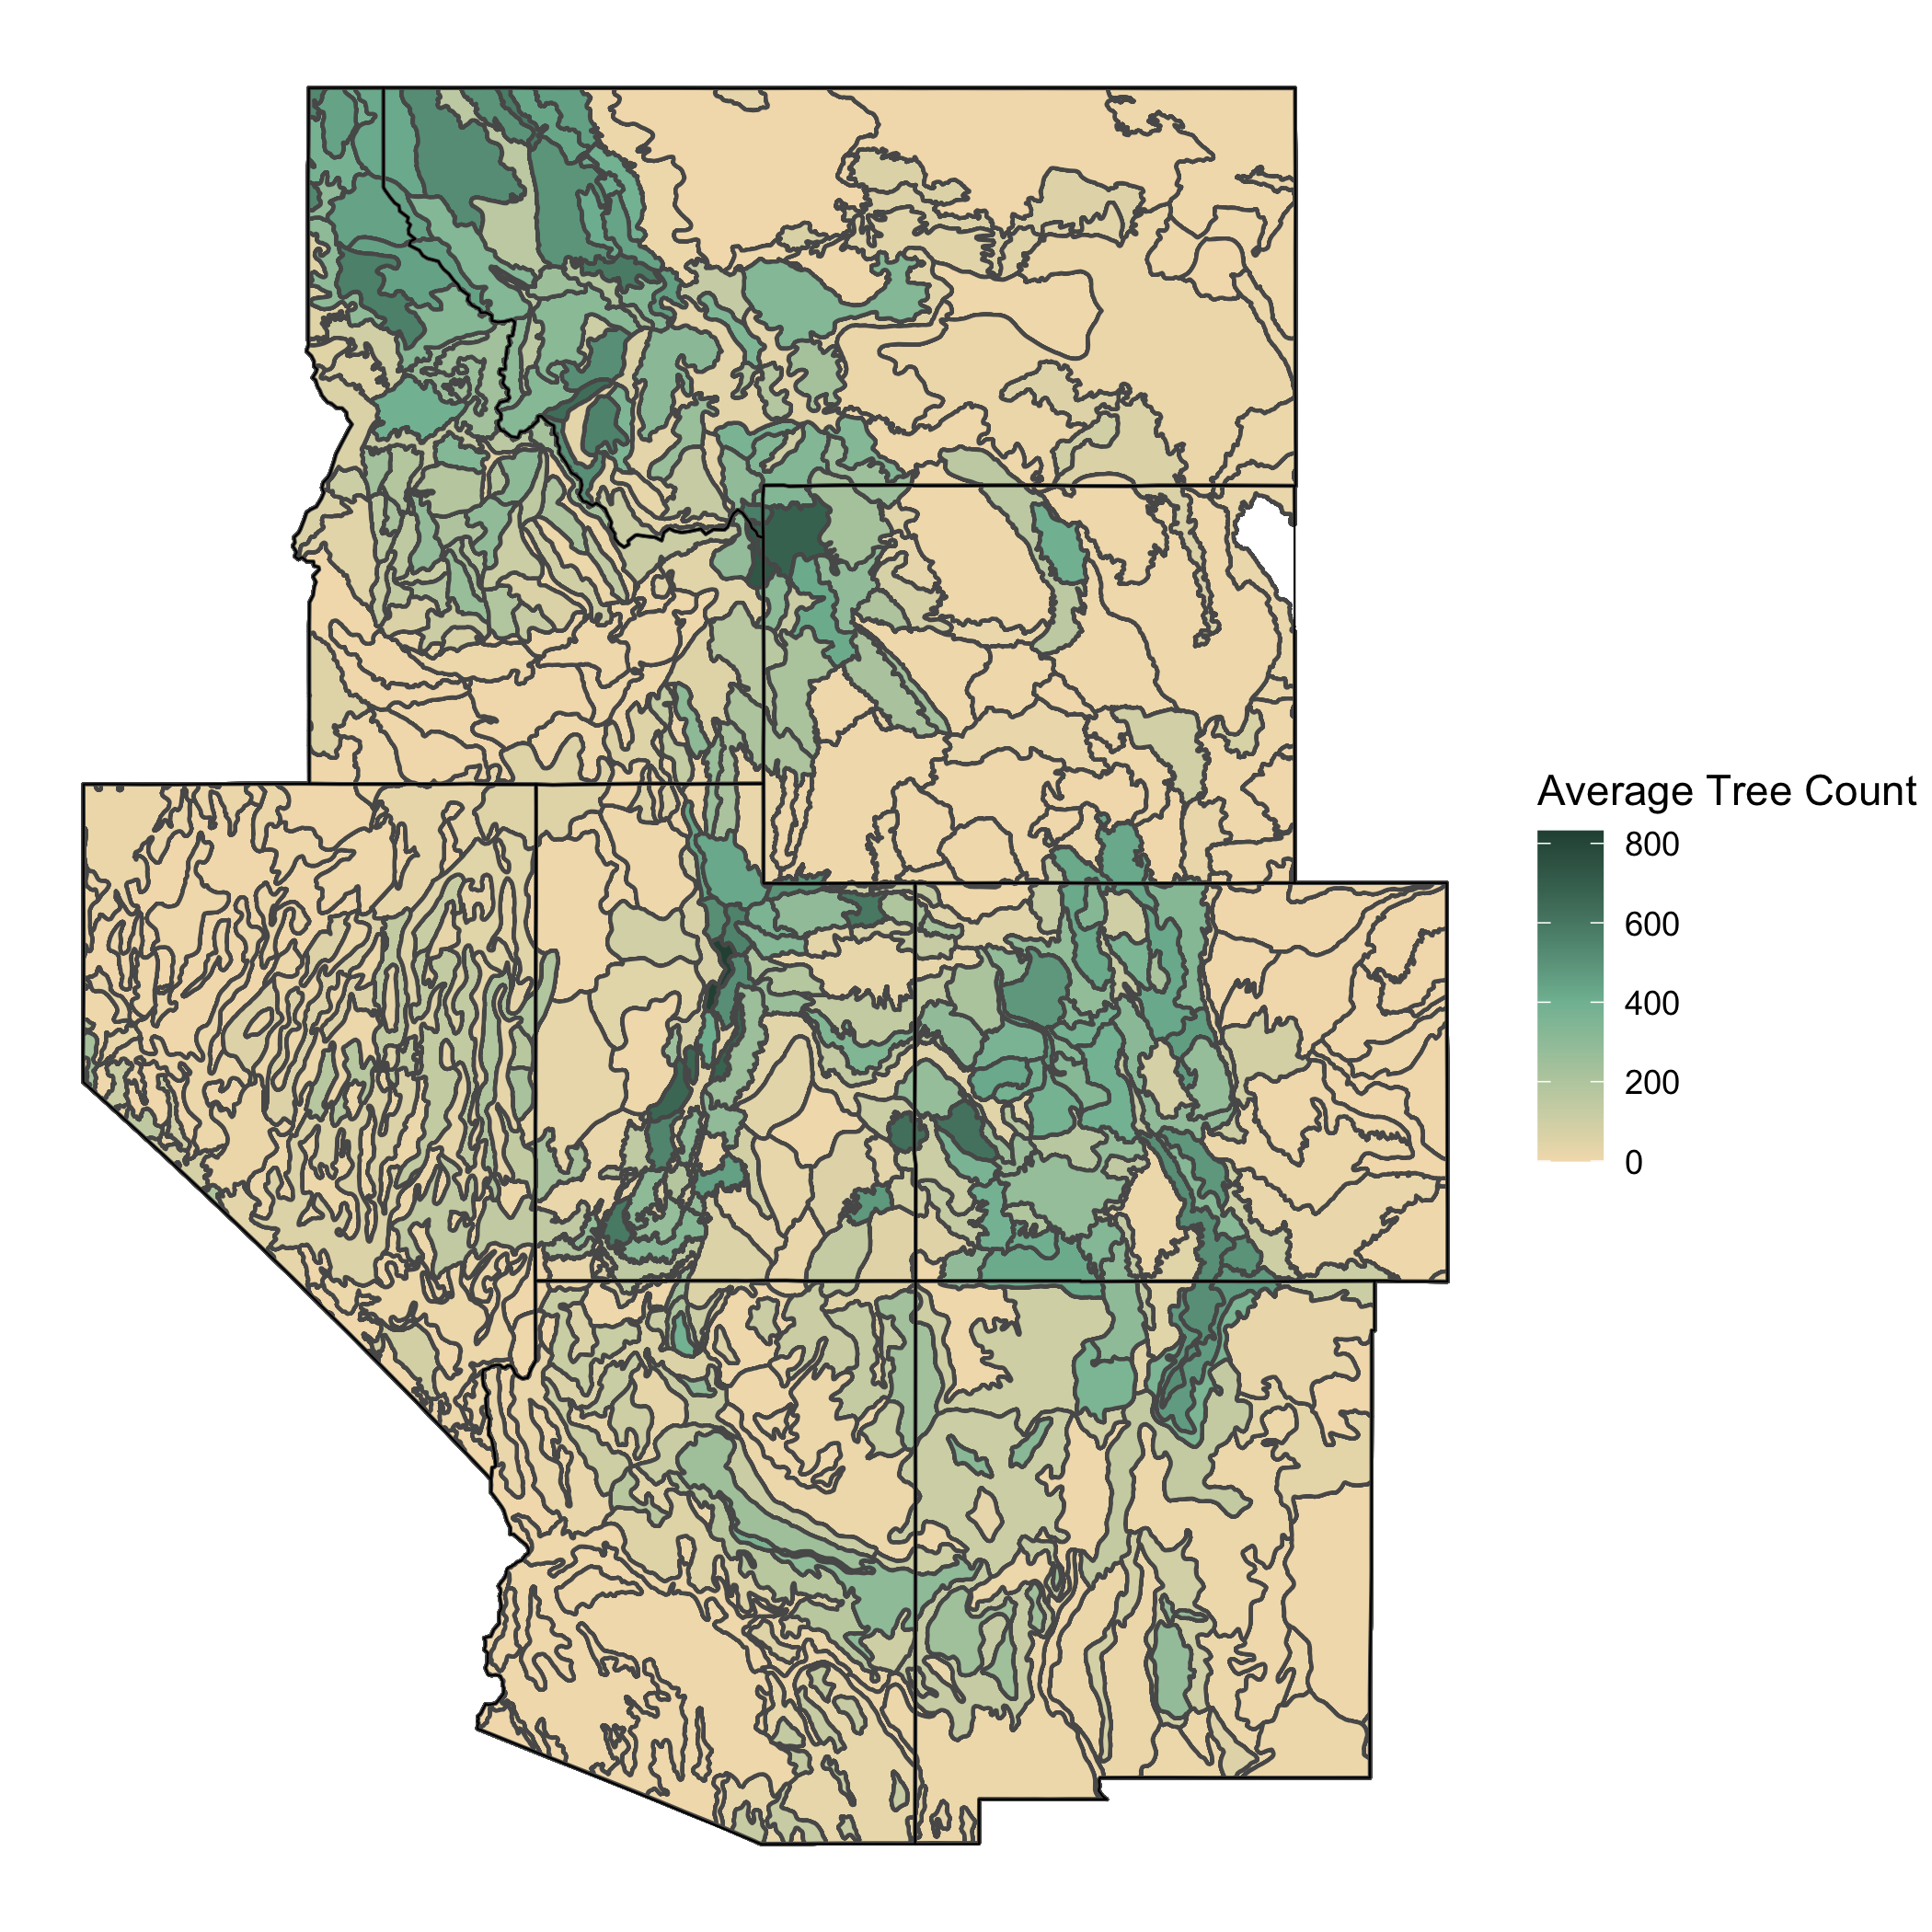
\includegraphics[width=0.65\linewidth]{figure/count} 

}

\caption{Mean tree count per acre in Interior West eco-subsections}\label{fig:unnamed-chunk-7}
\end{figure}
\begin{figure}

{\centering 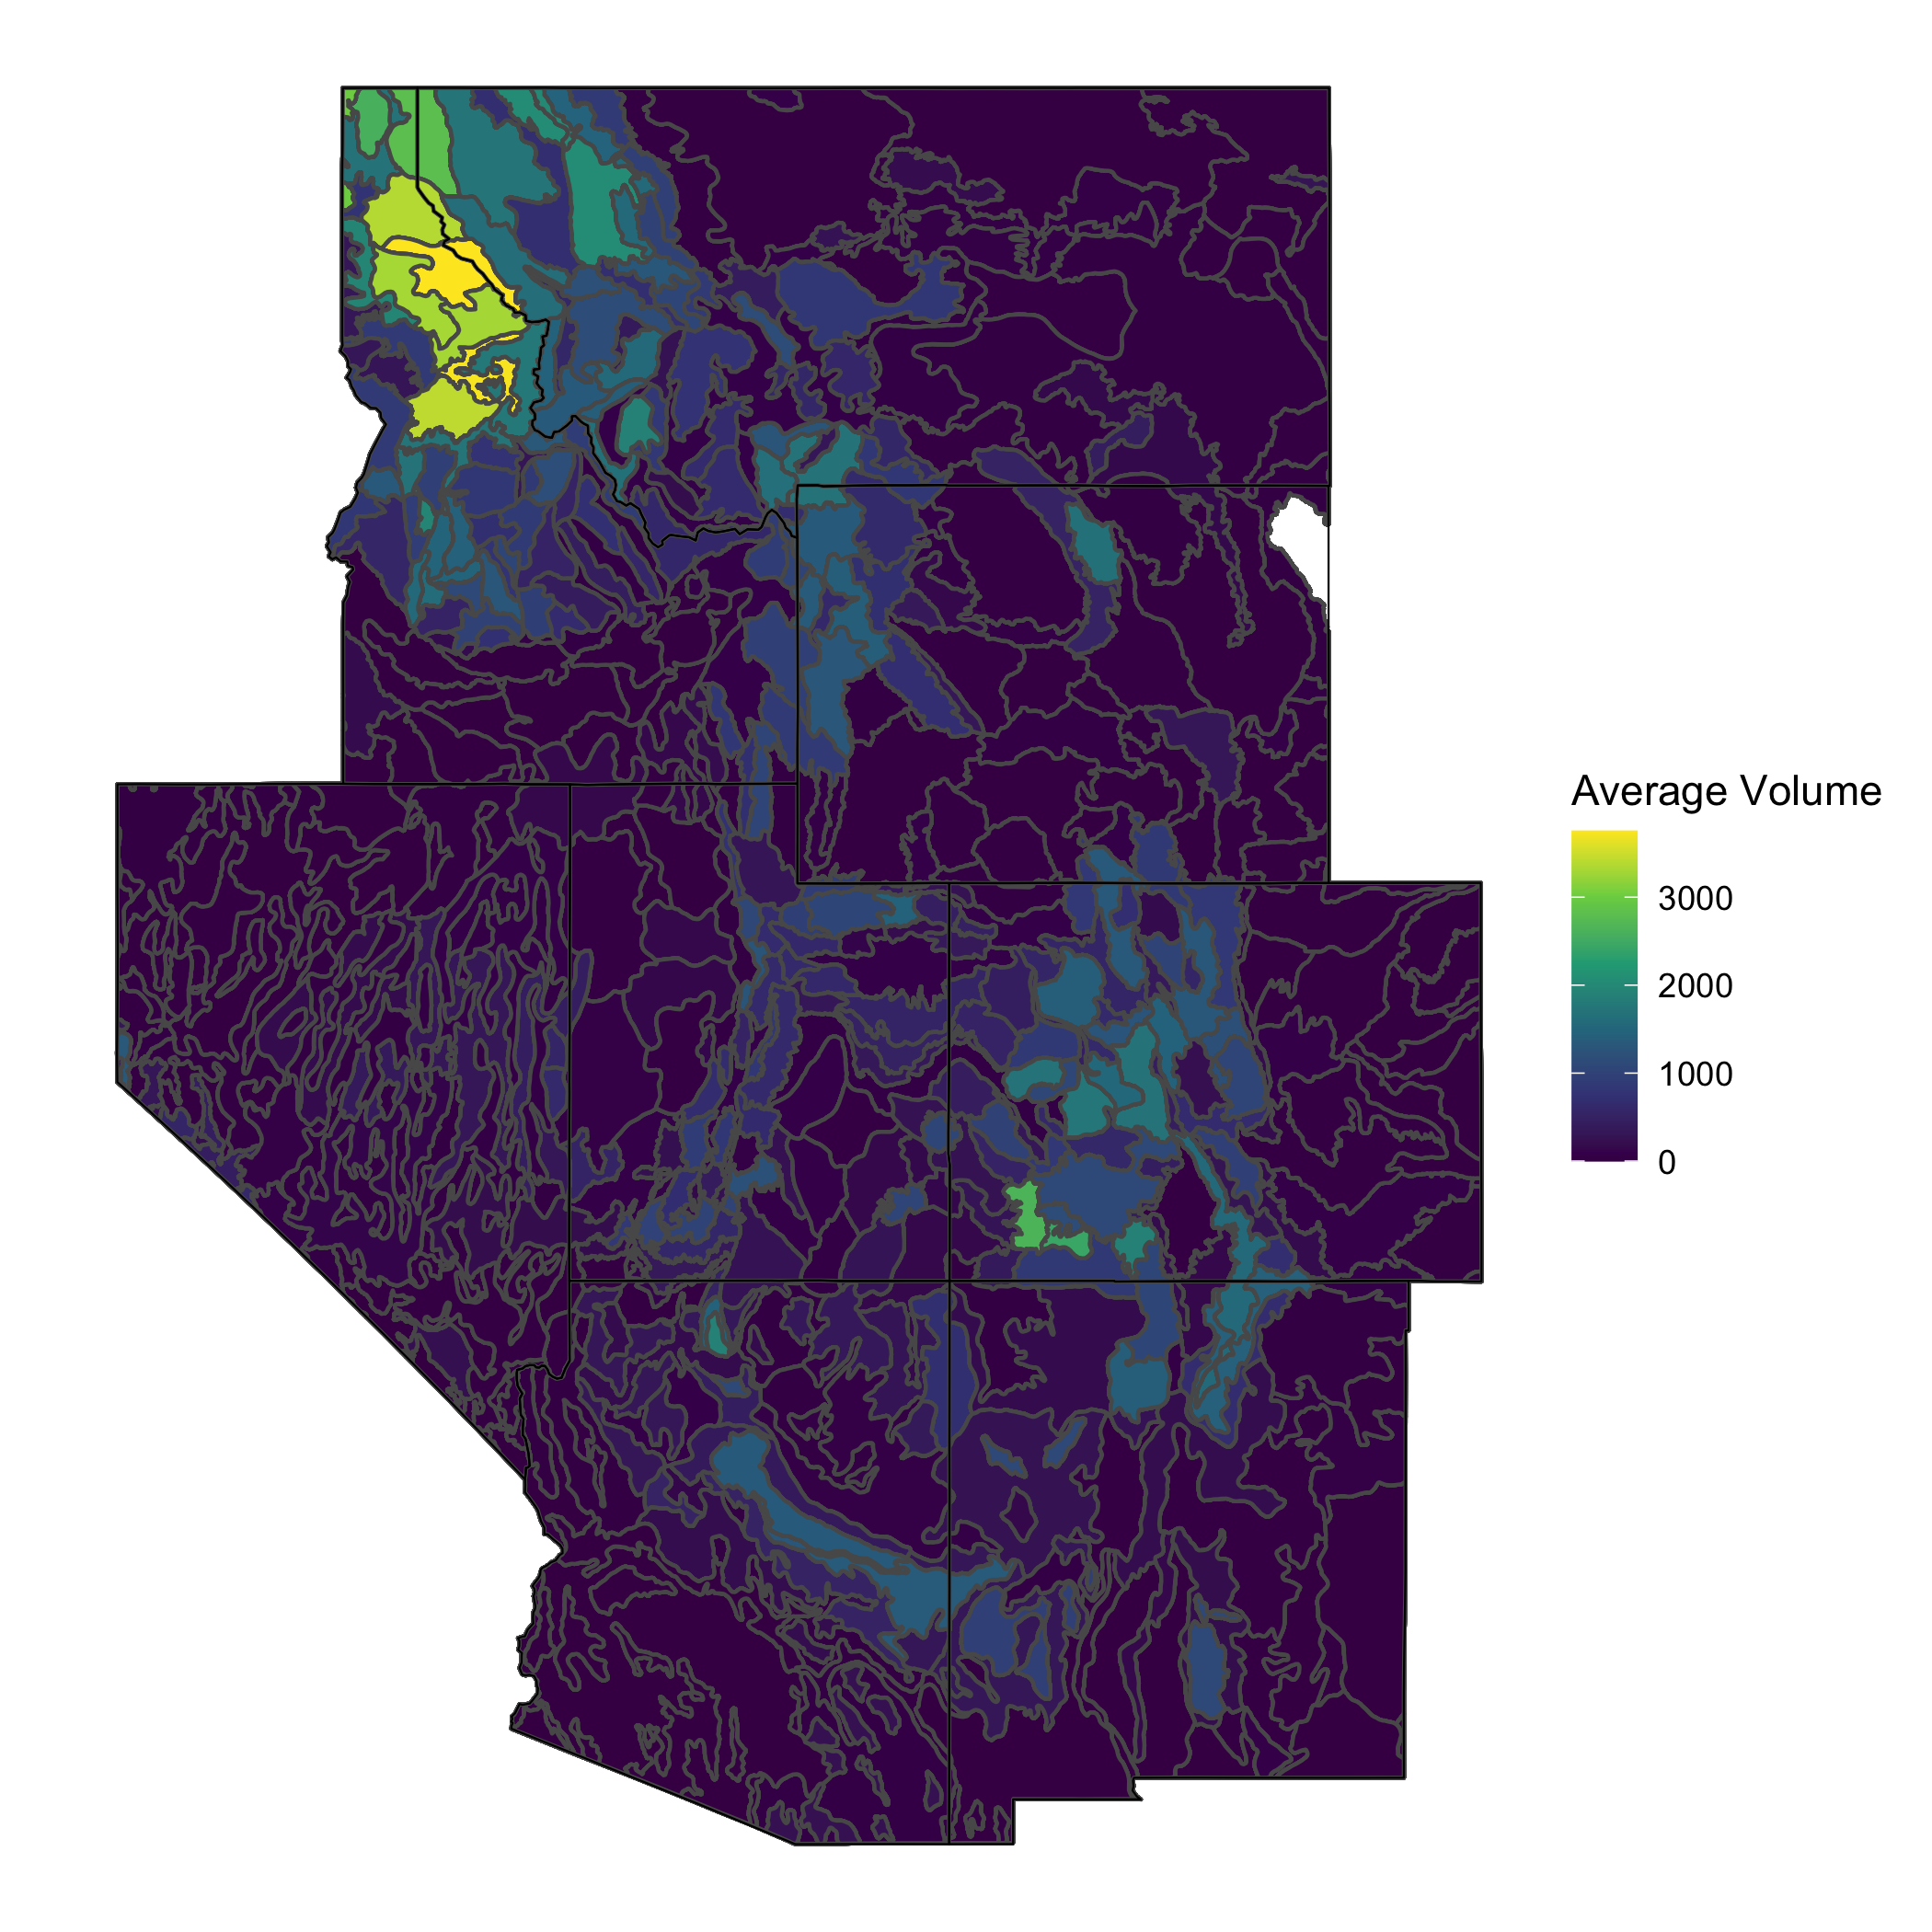
\includegraphics[width=0.65\linewidth]{figure/voln} 

}

\caption{Mean net volume in Interior West eco-subsections}\label{fig:unnamed-chunk-8}
\end{figure}
While we have four variables which we will model as response variables throughout the analyses, we also have one predictor variables which will be of much use to us. In particular, total tree canopy cover (coded as \texttt{nlcd11}.) This variable is remotely sensed, meaning that they were not collected by FIA crew members, but rather with aerial photography and/or satellite imagery. However, we will be using these variables to attempt to predict our response variables in order to understand how good of estimates we can make with this remote data that does not require as much effort to collect. Notably, we can consider this variable to contain the population totals for total canopy cover as the data is collected for the entire Interior West region.

To get a sense of a our predictor variable \texttt{nlcd11}, we will look at its distribution in the Northern Rocky Forest subset of our data compared to its distribution across the entire Interior West:
\begin{figure}

{\centering 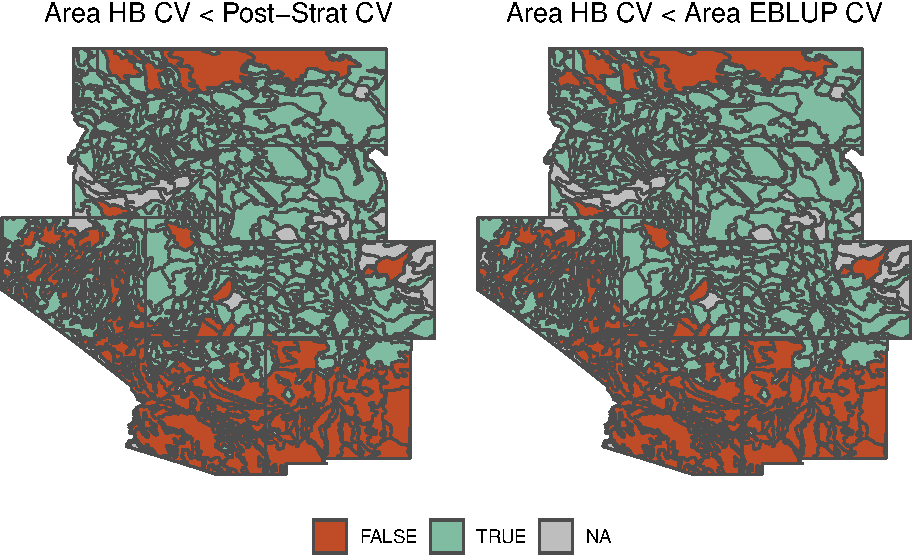
\includegraphics[width=432px]{thesis_files/figure-latex/unnamed-chunk-9-1} 

}

\caption[Total canopy cover in the M333 eco-province and Interior West]{Distribution of total canopy cover in the M333 eco-province (left) and the entire Interior West (right)}\label{fig:unnamed-chunk-9}
\end{figure}
Notably, the Northern Rocky Forest Province (M333) is much more forested than the Interior West, so we see much different distributions of total canopy cover in this subset of the data. Apart from making these histograms, we can also summarize the entire, unit-level data and see some summary statistics of our five key variables:
\begin{longtable}[t]{lrrrrrr}
\caption[Summary Statistics of Relevant Variables]{\label{tab:unnamed-chunk-10}Summary Statistics of Relevant Variables}\\
\toprule
Variable & Mean & SD & Median & 75th Percentile & Min & Max\\
\midrule
nlcd11 & 8.73 & 18.57 & 0 & 0.00 & 0 & 95.00\\
BIOLIVE\_TPA & 6.23 & 16.84 & 0 & 1.98 & 0 & 244.35\\
BALIVE\_TPA & 22.75 & 48.06 & 0 & 14.75 & 0 & 469.39\\
CNTLIVE\_TPA & 98.60 & 283.09 & 0 & 30.09 & 0 & 6677.93\\
VOLNLIVE\_TPA & 342.32 & 972.78 & 0 & 74.69 & 0 & 16435.55\\
\bottomrule
\end{longtable}
From this table, we can see how heavily skewed these key variables are, with all the variables having median of zero. This does not stop us from doing meaningful analyses though, as the sample size of this dataset is so large (\(n = 86085\)) and thus we have plenty of data to create models with.

Finally, we also have population data showing the proportion of each eco-subsection that is forested. This data allows us to create our post-stratified estimates which are discussed in detail in the following chapter.

\hypertarget{data-structure-hierarchy}{%
\section{Data Structure \& Hierarchy}\label{data-structure-hierarchy}}

As hinted at throughout earlier parts of the chapter, the data used in this thesis has a hierarchical structure, where eco-subsections are nested within eco-sections which are in turn nested within eco-provinces. Every plot has each level of granularity of location data recorded and this is what allows us to choose how far to borrow strength from other plots. We can see this structure of nested data by looking at a diagram depicting this data structure:
\begin{figure}

{\centering 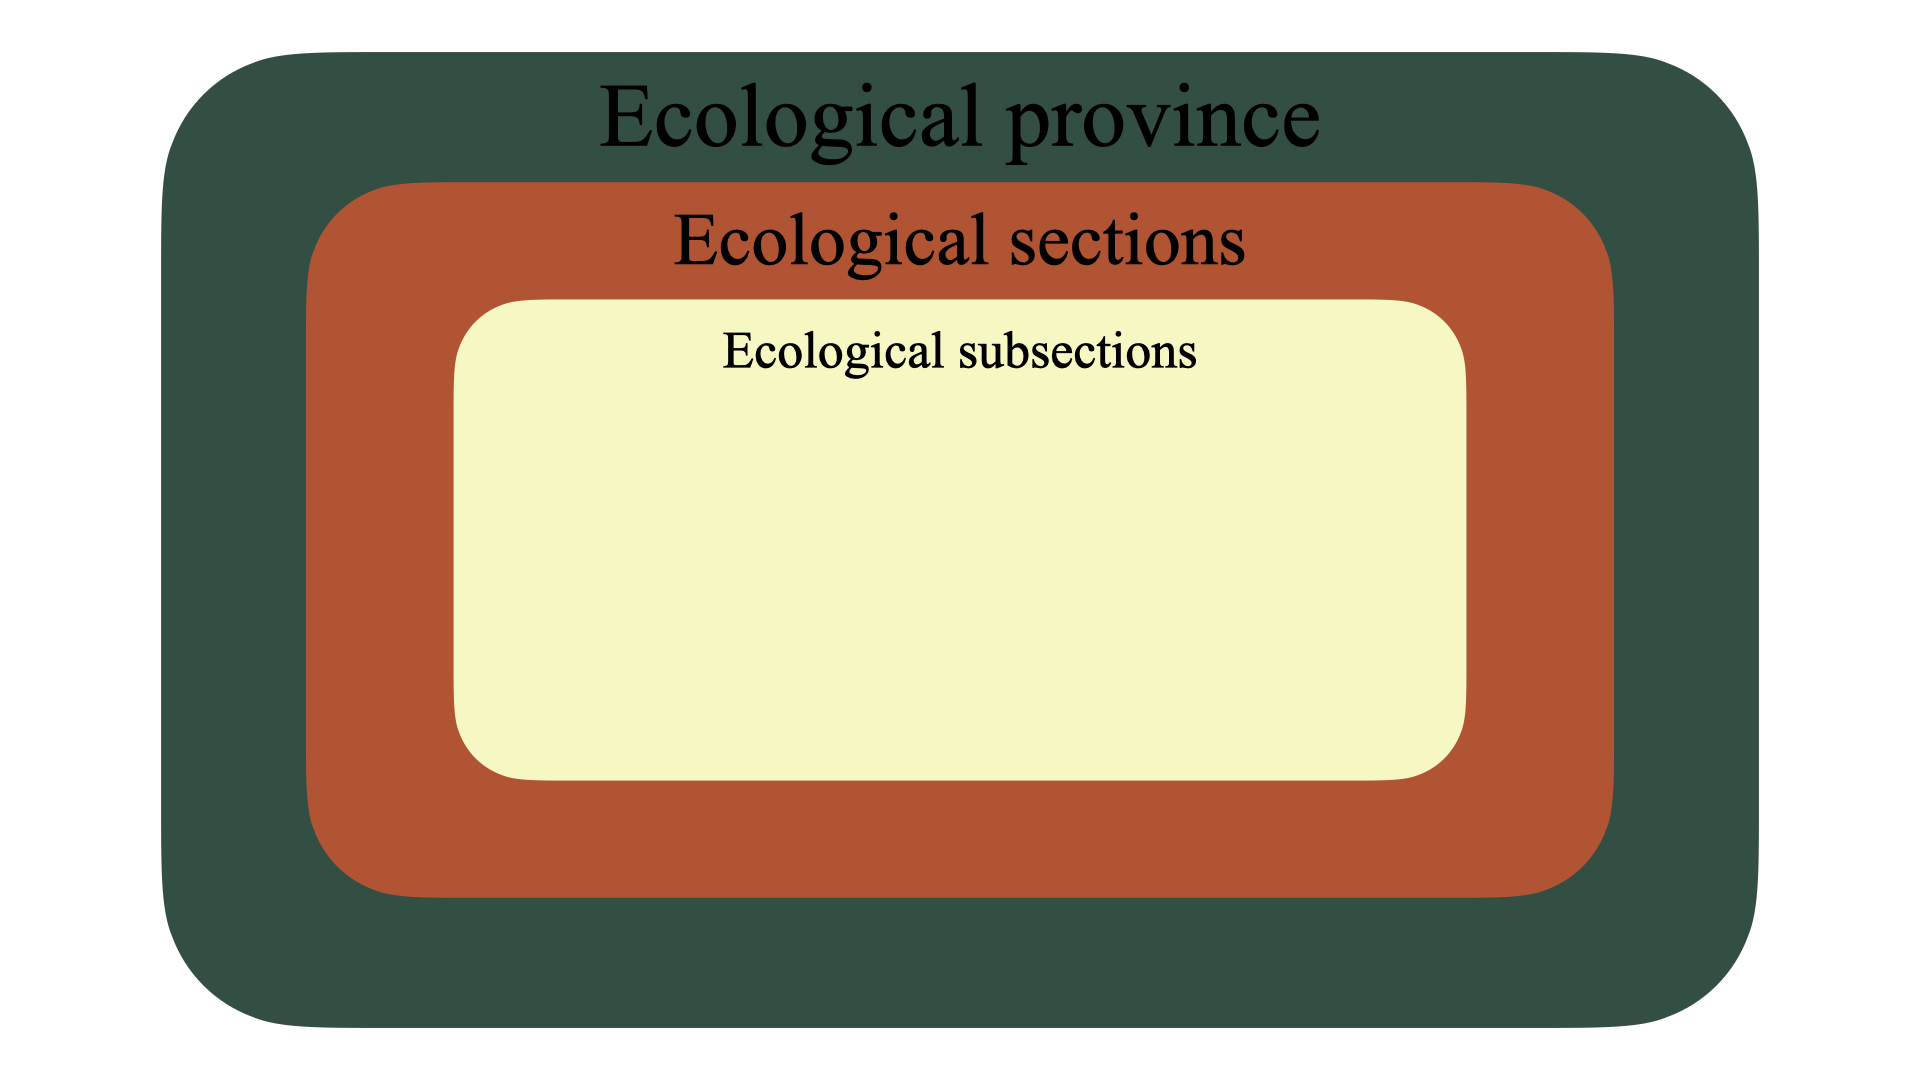
\includegraphics[width=1\linewidth]{figure/data-structure} 

}

\caption[The nested data structure of the Interior West]{The nested data structure of the Interior West. The green area is the eco-province which is divided into eco-sections (red area) which is in turn divided into eco-subsections (beige area).}\label{fig:unnamed-chunk-11}
\end{figure}
The largest motivation for hierarchical modeling in this particular application is that observations are more similar within the hierarchies which we split them into. To understand if this is true, we can do a preliminary analysis on the data by performing three-way ANOVAs for each key variable with predictors \texttt{province}, \texttt{section}, and \texttt{subsection}. For succinctness, we can look at the ANOVA results for one of the response variables, \texttt{BIOLIVE\_TPA}, but the other variables tell a very similar story in terms of homogeneity. By just looking at the MSE of the ANOVA results, we can see that we should expect more homogeneity within eco-subsections:
\begin{longtable}[]{@{}cccccc@{}}
\caption{Analysis of Variance Model (Biomass Response)}\tabularnewline
\toprule
\begin{minipage}[b]{0.15\columnwidth}\centering
term\strut
\end{minipage} & \begin{minipage}[b]{0.09\columnwidth}\centering
df\strut
\end{minipage} & \begin{minipage}[b]{0.13\columnwidth}\centering
sumsq\strut
\end{minipage} & \begin{minipage}[b]{0.10\columnwidth}\centering
meansq\strut
\end{minipage} & \begin{minipage}[b]{0.14\columnwidth}\centering
statistic\strut
\end{minipage} & \begin{minipage}[b]{0.14\columnwidth}\centering
p.value\strut
\end{minipage}\tabularnewline
\midrule
\endfirsthead
\toprule
\begin{minipage}[b]{0.15\columnwidth}\centering
term\strut
\end{minipage} & \begin{minipage}[b]{0.09\columnwidth}\centering
df\strut
\end{minipage} & \begin{minipage}[b]{0.13\columnwidth}\centering
sumsq\strut
\end{minipage} & \begin{minipage}[b]{0.10\columnwidth}\centering
meansq\strut
\end{minipage} & \begin{minipage}[b]{0.14\columnwidth}\centering
statistic\strut
\end{minipage} & \begin{minipage}[b]{0.14\columnwidth}\centering
p.value\strut
\end{minipage}\tabularnewline
\midrule
\endhead
\begin{minipage}[t]{0.15\columnwidth}\centering
province\strut
\end{minipage} & \begin{minipage}[t]{0.09\columnwidth}\centering
13\strut
\end{minipage} & \begin{minipage}[t]{0.13\columnwidth}\centering
6512457\strut
\end{minipage} & \begin{minipage}[t]{0.10\columnwidth}\centering
500958\strut
\end{minipage} & \begin{minipage}[t]{0.14\columnwidth}\centering
2921\strut
\end{minipage} & \begin{minipage}[t]{0.14\columnwidth}\centering
0\strut
\end{minipage}\tabularnewline
\begin{minipage}[t]{0.15\columnwidth}\centering
section\strut
\end{minipage} & \begin{minipage}[t]{0.09\columnwidth}\centering
54\strut
\end{minipage} & \begin{minipage}[t]{0.13\columnwidth}\centering
967169\strut
\end{minipage} & \begin{minipage}[t]{0.10\columnwidth}\centering
17911\strut
\end{minipage} & \begin{minipage}[t]{0.14\columnwidth}\centering
104.4\strut
\end{minipage} & \begin{minipage}[t]{0.14\columnwidth}\centering
0\strut
\end{minipage}\tabularnewline
\begin{minipage}[t]{0.15\columnwidth}\centering
subsection\strut
\end{minipage} & \begin{minipage}[t]{0.09\columnwidth}\centering
412\strut
\end{minipage} & \begin{minipage}[t]{0.13\columnwidth}\centering
2247965\strut
\end{minipage} & \begin{minipage}[t]{0.10\columnwidth}\centering
5456\strut
\end{minipage} & \begin{minipage}[t]{0.14\columnwidth}\centering
31.82\strut
\end{minipage} & \begin{minipage}[t]{0.14\columnwidth}\centering
0\strut
\end{minipage}\tabularnewline
\begin{minipage}[t]{0.15\columnwidth}\centering
Residuals\strut
\end{minipage} & \begin{minipage}[t]{0.09\columnwidth}\centering
85605\strut
\end{minipage} & \begin{minipage}[t]{0.13\columnwidth}\centering
14679154\strut
\end{minipage} & \begin{minipage}[t]{0.10\columnwidth}\centering
171.5\strut
\end{minipage} & \begin{minipage}[t]{0.14\columnwidth}\centering
NA\strut
\end{minipage} & \begin{minipage}[t]{0.14\columnwidth}\centering
NA\strut
\end{minipage}\tabularnewline
\bottomrule
\end{longtable}
These results allow us to conclude that it is reasonable to believe that observations within a given eco-province are more homogeneous than observations throughout the Interior West. Thus, if we want eco-subsection level estimates of variables, it makes sense to borrow information from other eco-subsections within the same province as each other. This data structure and homogeneity within provinces is what drives the analyses done henceforth in this thesis.

\hypertarget{methods}{%
\chapter{Methods}\label{methods}}

Currently, there are three main types of estimators used to estimate the value of forest attributes: direct, indirect with implicit models, and indirect with explicit models. Direct estimators are commonly thought of as the simplest estimators as they do not borrow strength across small areas for estimation. Direct estimators are hence easy to use and interpret, but we often do not get precise enough estimates with these estimators, in other words, they have high variance. Indirect estimators with implicit models borrow strength across small areas and produce estimates with implicit use of a model. These estimators decrease variance by providing a link to related small areas through supplementary data (Rao, 2014). Finally, indirect estimators that make explicit use of a model, or ``model-based estimators'', aim to reduce variance in estimates by using auxiliary data and making specific allowance for between area variation. As explained in Rao (2014), these model-based estimators have significant advantages over direct estimators and implicit indirect estimators. Notably, model diagnostics can be used, small area-specific measures of precision can be attained (in our case, we compare the coefficient of variation between estimators), and we can used mixed or hierarchical models.

This thesis explores the application of two less commonly applied model-based estimators, the hierarchical Bayesian unit-level model and the hierarchical Bayesian area-level model. We compare these novel Bayesian models to the frequentist EBLUP unit- and area-level models and two common direct estimators, the mean and the post-stratified estimator. To compare these estimators, we will apply them over many ecological provinces in the Interior West and study their performance when considering four response variables with one explanatory variable.

In order to explore these estimators in depth, we must introduce notation relevant to them. First of all, our indices will work as follows: \(i\) indexes over units sampled; \(j\) indexes over eco-subsections or ``small areas''; and \(k\) indexes over strata. Now, we are interested in estimating the mean of some study variable \(y\), such as trees per acre or biomass, in a small area. So, let \(\mu_{y_j}\) be the population mean of the study variable in eco-subsection \(j\) in the Interior West. To denote the estimate produced of \(\mu_{y_j}\) we will use \(\hat\mu_{y_j}\) with a superscript denoting which estimator is being used. In summary, each of our estimators aims to estimate \(\mu_{y_j}\), the population mean of some study variable in the \(j\)th eco-subsection and our estimated value is denoted by \(\hat\mu_{y_j}\). We also must introduce \(s_j\), which is a set. The set \(s_j\) includes all units sampled within eco-subsection \(j\). We also introduce \(U_j\), the set of all the area in subsection \(j\). The ``\(U\)'' is chosen as it stands for ``universe.'' Also, we introduce \(n_j\), this denotes the number of sampled units within an eco-subsection \(j\), i.e.~the cardinality of \(s_j\).

\hypertarget{direct-estimation}{%
\section{Direct Estimation}\label{direct-estimation}}

There are two direct estimators that we will explore throughout this thesis: the sample mean (a.k.a. the Horvitz-Thompson estimator) and the post-stratified estimator. While the sample mean is an intuitive choice for estimating the population mean of a variable of interest \(y\), the post-stratified estimator helps correct for over- and under-sampling of forested areas. We will now explore both of these estimators in depth.

\hypertarget{the-horvitz-thompson-estimator}{%
\subsection{The Horvitz-Thompson Estimator}\label{the-horvitz-thompson-estimator}}

What might be the most intuitive approach to estimating the population mean \(\mu_{y_j}\) is taking the sample mean, i.e.~using the ``Horvitz-Thompson estimator'' as foresters like to say. This estimator can be expressed as follows:
\begin{align}
\hat\mu_{y_j}^{HT} = \frac{1}{n_j} \sum_{i \in s_j} y_i
\end{align}
The variance estimate, \(S\), for Horvitz-Thompson estimator is calculated by:
\begin{align}
S_j^{2} = \frac{1}{n_j-1} \sum_{i \in s_j} \Big(y_i - \hat\mu_{y_j}^{HT}\Big)^2
\end{align}
Recall that the Horvitz-Thompson estimator is just taking the mean of the study variable of interest, \(y\). Note that \(y_i\) represents the value of the study variable in the \(i\)th unit sampled of eco-subsection \(j\). This estimator is useful as it is easy to compute and does not require any auxiliary information. However, the Horvitz-Thompson estimator high variance relative to other estimators we will discuss and it is biased unless we have sampled the correct proportion of forested areas. The post-stratified estimator begins to address both the bias and variance of the Horvitz-Thompson estimator.

\hypertarget{the-post-stratified-estimator}{%
\subsection{The Post-Stratified Estimator}\label{the-post-stratified-estimator}}

The post-stratified estimator is very similar to the Horvitz-Thompson estimator however, as stated above, it addresses bias and variance that occurred from using the Horvitz-Thompson estimator. While decreasing bias and variance seems like a no cost solution to some of our problems, the post-stratified estimator requires auxiliary information in order to be used. The post-stratified estimator is a weighted sum of two Horvitz-Thompson estimators: one Horvitz-Thompson estimator giving the estimate of the mean in sampled units which are forested and the other Horvitz-Thompson estimator in non-forested areas. We then weight these estimates by the true proportion of area in the eco-subsection of interest that is forested. Note that while we are using auxiliary information such as the true proportion of forested area in the eco-subsection of interest and whether or not the sampled units were forested areas or not, both of these pieces of information only consider the eco-subsection of interest. Therefore, since information is not used from outside of the eco-subsection of interest, the post-stratified estimator is still within the family of direct estimators. We can represent the post-stratified estimator as follows:
\begin{align}
\hat\mu_{y_j}^{PS} = \sum_{k=1}^{2} w_k \cdot \hat\mu_{y_{j,k}}^{HT}
\end{align}
Recall that \(k\) indexes over our strata, which in this case is forested and non-forested sampled units. We also have \(w_k\), which is a survey weight entirely decided by the true proportion of eco-subsection \(j\) which is forested. For example, if eco-subsection \(j\) was 80\% forested, we would have \(w_1 = 0.8\) and \(w_2 = 0.2\). Therefore if we had under-sampled forests at only 60\% of our samples, we correct this under-sampling with our survey weights and this results in a design-unbiased estimate of \(\mu_{y_j}\).

The post-stratified estimator is a great alternative to the Horvitz-Thompson estimator when auxiliary information is available, and in that situation there is not a justifiable reason to pick the Horvitz-Thompson estimator over the post-stratified estimator as the direct estimator of choice. We have access to the information needed to compute the post-stratified estimate in the Interior West so we will primarily be comparing our indirect estimators to the post-stratified estimator in our results. Also, our area-level indirect model-based estimators will be based on the post-stratified estimate.

\hypertarget{implicit-model-based-indirect-estimation}{%
\section{Implicit Model Based Indirect Estimation}\label{implicit-model-based-indirect-estimation}}

Often times it is the case that direct estimation techniques do not provide sufficiently small standard errors to be able to make informative inferences at the small area level. That is the case in our situation, as the FIA's survey design was based around making inferences at larger levels than eco-subsections. One relatively simple approach to decreasing variance of estimates at a small area level is to use auxiliary data from surrounding areas to help attain the estimate in the small area of interest. This process is called borrowing strength. It is very similar to the borrowing of strength outlined in Figures \ref{fig:hbu-diagram} and \ref{fig:hba-diagram}, however, in the case of implicit model based indirect estimation we do not allow for between-area variation of explanatory variables. That is, we may borrow strength across small areas by using auxiliary data, but this auxiliary data must be aggregated and have the same effect on each small area within a designated area (in our case, this is the ecological province).

We introduce two implicit model based indirect estimators commonly used when auxiliary data is available at the unit- and area-levels. These estimators are not used in the final analyses done in this thesis. However, they are crucial building blocks for understanding the frequentist EBLUP models we discuss and implement. First we discuss a common estimator used when area-level auxiliary data is available and then a common estimator for unit-level auxiliary data.

\hypertarget{using-area-level-auxiliary-data}{%
\subsection{Using Area-level Auxiliary Data}\label{using-area-level-auxiliary-data}}

When we choose to use area-level auxiliary data and implicit model based indirect estimation, Rao (2014) suggests the regression-synthetic estimator. Here, in order to estimate our parameter of interest, \(\mu_{y_j}\), we fit an ordinary least squares linear regression on our \(p\) auxiliary variables over each small area in our large domain:
\begin{align}
\hat\mu_{y_j}^{RS} = \hat\beta_0 + \hat\beta_1 x_{j,1} + \cdots + \hat\beta_p x_{j,p}
\end{align}
We note that the \(\hat \beta\)'s are calculated through standard methods of ordinary least squares and in the case of our analysis \(p=1\). Further, it is important to recognize that in the case of the regression-synthetic estimator each small area receives the same \(\hat\beta\)'s. This is the realization of the requirement that the auxiliary information must have the same effect on each small area.

\hypertarget{using-unit-level-auxiliary-data}{%
\subsection{Using Unit-level Auxiliary Data}\label{using-unit-level-auxiliary-data}}

An approach to implicit model based indirect estimation when unit-level auxiliary information is available is to use the survey regression estimator.
\begin{align}
\hat \mu_{y_j}^{SR} = \overline y_j + (\overline X_j - \overline x_j)^T \hat\beta
\end{align}
\hypertarget{explicit-model-based-indirect-estimation}{%
\section{Explicit Model Based Indirect Estimation}\label{explicit-model-based-indirect-estimation}}

Often times, implicit model based indirect estimators still do not reduce variance enough to give us estimates with reasonable standard errors. However, we can turn to explicit model based indirect estimation in order to combat this issue further. Explicit model based indirect estimators are extremely useful when relevant auxiliary data is available and we would like to allow for between-area variation of these auxiliary variables. By allowing for this between-area variation our models should fit to the data better given that there is truly between-area variation in the population. In the case of forests across a large portion of the United States, this assumption is very reasonable and one could attribute this variation to a number of factors such as temperature, humidity, or even elevation. Rather than attempting the daunting and nonsensical task of collecting data to fully explain this between-area variation, we fit a mixed model.

In small area estimation it is most common that the mixed model estimator used is one of the EBLUP estimators: either the unit- or area-level variant depending on the resolution of auxiliary data preferred. The EBLUP estimators are unbiased given the modeling assumptions are met, similar to the post-stratified estimator. We will now explore the model specifications of these EBLUP estimators at the unit- and area-level.

\hypertarget{the-unit-level-eblup}{%
\subsection{The Unit-level EBLUP}\label{the-unit-level-eblup}}

In the case of the unit-level EBLUP, we first fit a varying-intercepts linear mixed model at the unit-level:
\begin{align}
y_{i,j} = \vec x_{i,j}^T \vec \beta + \nu_j + e_{i,j}
\end{align}
with
\[
 \newcommand\myeq{\stackrel{\mathclap{\normalfont\mbox{s}}}{~}}
\nu_j \stackrel{\text{iid}}{\sim} \text{N}(0,~ \sigma^2_{\nu}), \quad e_{i,j} \stackrel{\text{ind}}{\sim}\text{N}(0, k^2_{i,j}\sigma^2_e).
\]
Rao (2014) derives the unit-level EBLUP estimator from (the above eqn) fit in the frequentist paradigm as the weighted average of the survey regression estimator and the regression-synthetic estimator:
\begin{align}
\hat \mu_{y_j}^{FRU} = \hat \gamma_j \hat\mu_{y_j}^{SR} + (1 - \hat \gamma_j) \hat\mu_{y_j}^{RS}
\end{align}
where
\begin{align}
\hat\gamma_j = \sigma^2_\nu / (\sigma^2_\nu + \sigma^2_e / a_i)
\end{align}
(say what \(a_i\) is from Rao around 7.1.3, 7.1.4)

\hypertarget{the-area-level-eblup}{%
\subsection{The Area-level EBLUP}\label{the-area-level-eblup}}

EQN 6.1.1 (the linear mixed model formula at the area level):

In order to obtain the EBLUP estimator at the area level, we first fit the following linear mixed model:
\begin{align}
\hat\mu_{j}^{PS} = z_j^T \beta + b_j \nu_j + e_j
\end{align}
Next, Rao (2014) derives the commonly expressed form of the EBLUP estimator:

The area-level EBLUP estimator is expressed by Rao (2014) as a weighted average of the direct estimator and the regression-synthetic estimator:
\begin{align}
\hat \mu_j^{FRA} = \hat\gamma_j \hat\mu_j^{PS} + (1 - \hat\gamma_j) \hat\mu_j^{RS} \label{eq:eblup-area-weight}
\end{align}
where
\begin{align}
\hat \gamma_j = \hat \sigma_\nu^2 b_j^2 / (\psi_j + \hat\sigma_\nu^2 b_j^2)
\end{align}
(I need to define a lot of these quantities. Trying to find the best way to do this without pulling every little thing from Rao)

\hypertarget{a-hierarchical-bayesian-approach}{%
\section{A Hierarchical Bayesian Approach}\label{a-hierarchical-bayesian-approach}}

So far in this chapter, we have explored common frequentist approaches to small area estimation. However, the research goal of this thesis is to study the performance of the hierarchical Bayesian model for small area estimation. With a hierarchical Bayesian model, we derive the posterior distribution of our variable of interest with either Markov Chain Monte Carlo (MCMC) methods or through numerical integration. We do this by considering both the data (likelihood) and prior distributions. This allows us to use Bayes' Theorem in order to attain our posterior.

Before we introduce the models used in this thesis, we must introduce some notation. Consider a set of model parameters \(\lambda\), the data \(y\), and the parameter of interest \(\mu\) for each eco-subsection. We would like to obtain the distribution of \(f(\mu ~\vert~ y)\), i.e.~the distribution of our parameter of interest, \(\mu\), given our data \(y\). Rao (2014) shows that we can obtain this desired posterior density by first obtaining the posterior density of \(\mu\) and \(\lambda ~\vert~ y\),
\begin{align}
f(\mu,~ \lambda ~\vert~ y) = \frac{f(y, \mu ~\vert~ \lambda) f(\lambda)}{f(y)}
\end{align}
and then integrating over \(\lambda\):
\begin{align}
f(\mu ~\vert~ y) = \int f(\mu,~ \lambda ~\vert~ y) \text{d}\lambda.
\end{align}
Depending on the functional form of the densities we must integrate to obtain our posterior, it is often easier to approximate the distribution with MCMC methods. However, in the case of this thesis, we use numerical integration to extract exact posterior densities from our likelihood and priors. We will now give the form of both the unit- and area-level hierarchical Bayesian models used in this thesis.

\hypertarget{the-unit-level-hierarhcical-bayesian-model}{%
\subsection{The Unit-level Hierarhcical Bayesian Model}\label{the-unit-level-hierarhcical-bayesian-model}}

\hypertarget{the-area-level-hierarichical-bayesian-model}{%
\subsection{The Area-level Hierarichical Bayesian Model}\label{the-area-level-hierarichical-bayesian-model}}

\hypertarget{results}{%
\chapter{Results}\label{results}}

This chapter addresses the performance of the six estimators in this thesis: the sample mean, the post-stratified estimator, the unit-level EBLUP, the area-level EBLUP, the unit-level hierarchical Bayesian estimator, and the area-level hierarchical Bayesian estimator.

We used the R statistical software to compute our results (R Core Team, 2020). The sample mean was computed using the \emph{sae} (Molina \& Marhuenda, 2015). The post-stratified estimates were computed using \emph{mase} (McConville, Tang, Zhu, Cheung, \& Li, 2018). The frequentist EBLUP estimates were computed using \emph{sae} (Molina \& Marhuenda, 2015). The hierarchical Bayesian estimates were computed using \emph{hbsae} (Boonstra, 2012). The results were tidied, processed, and visualized using many \emph{tidyverse} packages (Wickham et al., 2019). Our data spans the entire Interior West, however we were forced to exclude a few eco-provinces. Namely two eco-provinces with a very small number of eco-subsections which caused errors in producing the unit-level hierarchical Bayesian estimates and eco-subsections with either none or very close to no sampled areas with non-zero values for our variables of interest. While this is disappointing, we still were able to fit these estimators to the great majority of our data.

This thesis uses all six of these estimators to produce estimates for basal area (square-foot), tree count per acre, above-ground biomass (lbs), and net volume (\(\text{ft}^3\)). The EBLUP and hierarchical Bayesian estimators use one explanatory variable, total canopy cover, to produce estimates. Our estimation occurs at the eco-subsection level, and thus we have 10,176 estimates produced (six estimators, four response variables, and 424 eco-subsections).

We are generally concerned with producing estimates that have both low variance and low bias. This chapter primarily aims to answer questions regarding these two quantities. In order to do so, we will summarize our findings both globally and by briefly examining a subset of our results in the Northern Rocky Forest. This subset examination allows us to dig in to results without much aggregation or incomprehensible plots due to the large amount of results we have. We explore both metrics and visualizations of variance and bias across the interior west in order to deeply understand the performance of our estimators. This thesis is, in many ways, a study navigating the bias-variance trade-off in depth in a real world setting. While quantifying variance of estimates is a generally straightforward task, producing an accurate depiction of bias is extremely difficult without knowing population parameters.

\hypertarget{estimator-performance}{%
\section{Estimator Performance}\label{estimator-performance}}

We will now investigate the performance of the six estimators used in this thesis. In order to explore variance, the primary metric we use is the coefficient of variation (\(CV\)). This metric, for each estimator, is defined as the standard deviation of our estimate divided by the sample mean in that small area (\(\hat \mu_{y_j}^{HT}\)). This allows us to normalize our variation across different response variables and areas that are more or less forested. We can express the coefficient of variation as follows:
\begin{align}
CV_{y_j} = \frac{\hat\sigma_{y_j}}{\hat\mu_{y_j}^{HT}}
\end{align}
It is notable that when the mean of the variable of interest is small, we will sometimes get strangely large coefficients of variation for estimators that borrow strength. This phenomenon can generally be thought of as more to do with intrinsic (and often very good) qualities of the estimator rather than correlation with poor performance of the estimator when the sample mean is small. Notably, estimators which borrow strength to a large degree in situations where the sample mean is low and the areas which we borrow strength from have significantly higher values will have higher variance due to this heterogeneity. We will explore this idea in depth further on in this chapter.

In order to visualize the coefficients of variation in an appealing way, we have filtered out all observations greater than one in the following plot:
\begin{figure}

{\centering 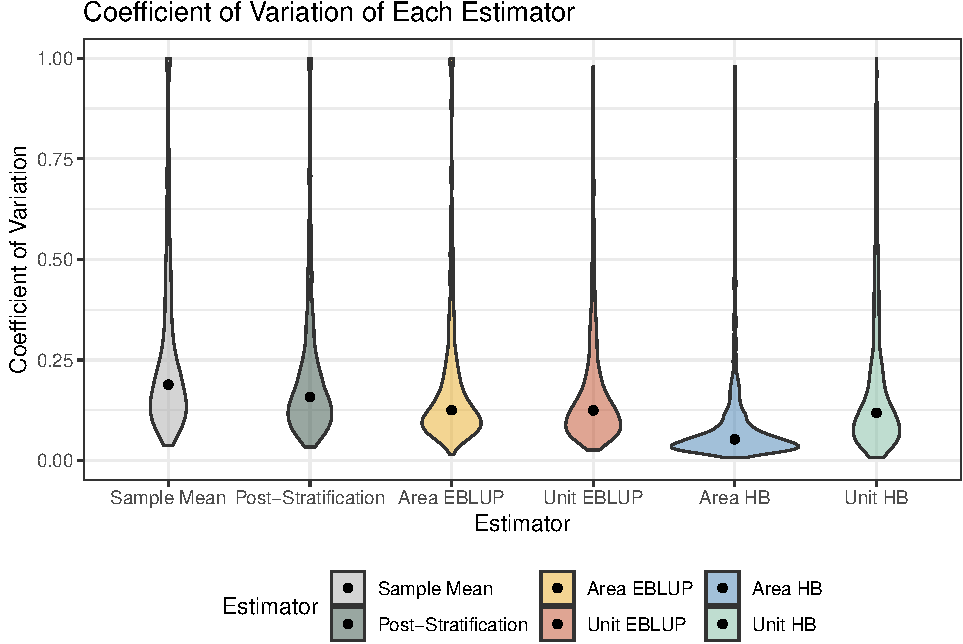
\includegraphics[width=1\linewidth]{thesis_files/figure-latex/cov-violin-1} 

}

\caption[Distribution of the coefficient of variation of each eastimator]{Distribution of the coefficient of variation of each eastimator. The black dot in each violin segment represents the median coefficient of variation value. The width of the violin segments corresponds to the density of points in the given value range. Values greater than 1 truncated in plot, however still considered in median calculation.}\label{fig:cov-violin}
\end{figure}
Figure \ref{fig:cov-violin} shows the coefficient of variation for each estimator. We see a slight reduction in the coefficient of variation when moving from the sample mean to post-stratification, and a decently large reduction in variation when adding auxiliary data with either EBLUP estimator. We also see that the unit-level hierarchical Bayesian estimator performs quite similarly to the unit-level EBLUP. This makes sense as at the unit-level we have so much data that it outweighs the contribution of any priors significantly. Finally, we see a huge reduction in the coefficient of variation compared to all other estimators when we fit the area-level hierarchical Bayesian estimator. The median coefficient of variation for this area-level hierarchical Bayesian estimator (0.055) is less than half of the next best performing median coefficient of variation from the area-level EBLUP (0.125). Examining the quantiles of these estimator's coefficient of variation continues to show the superiority of the area-level hierarchical Bayesian estimator while also demonstrating the metric's tendency to have some extremely large values:
\begin{longtable}[t]{lrrrrr}
\caption[Coefficient of Variation Quantiles]{\label{tab:quantile-table}Quantiles of Each Estimator's Coefficient of Variation}\\
\toprule
Estimator & 0\% & 25\% & 50\% & 75\% & 100\%\\
\midrule
Sample Mean & 0.038 & 0.123 & 0.189 & 0.318 & 1.000\\
Post-Stratification & 0.034 & 0.105 & 0.158 & 0.255 & 1.000\\
Area EBLUP & 0.015 & 0.087 & 0.125 & 0.213 & 0.999\\
Unit EBLUP & 0.026 & 0.085 & 0.131 & 0.244 & 52.408\\
Area HB & 0.007 & 0.034 & 0.055 & 0.112 & 56.401\\
\addlinespace
Unit HB & 0.008 & 0.078 & 0.150 & 0.486 & 299.673\\
\bottomrule
\end{longtable}
While Figure \ref{fig:cov-violin} and Table \ref{tab:quantile-table} gives us a good sense of the distribution, we must acknowledge that we truncated some values in Figure \ref{fig:cov-violin} and further investigate why the coefficient of variation tends to get very large in some cases. By examining the distribution and performance of the coefficients of variation by truncating the tails in Figure \ref{fig:cov-violin} we are able to gain insight that would be much harder to see while including the tails. Now, we can look more in depth at the tails of these distributions. Four estimators had coefficients of variation that exceeded 1. The below table shows the count and proportion of each:
\begin{longtable}[t]{lrr}
\caption{\label{tab:over-one}Coefficient of variation estimates greater than one}\\
\toprule
Estimator & Count & Proportion\\
\midrule
Post-Stratification & 0 & 0.000\\
Area EBLUP & 0 & 0.000\\
Sample Mean & 0 & 0.000\\
Area HB & 81 & 0.048\\
Unit EBLUP & 103 & 0.061\\
\addlinespace
Unit HB & 289 & 0.170\\
\bottomrule
\end{longtable}
We see that there are three estimators with coefficient of variations greater than one. Both the frequentist and hierarchical Bayesian unit-level estimators have many values greater than one, and the area-level hierarchical Bayesian has some as well. To understand why these particular estimators have many estimates greater than one, we first need to explore the small areas which have these coefficient of variation values. To do so, we can examine the mean response value for estimates where the coefficient of variation is greater than one and when it is less than one.
\begin{longtable}[t]{lrr}
\caption{\label{tab:covg1l1}Mean Estimates Where Coefficent of Variation is Greater Than and Less Than One}\\
\toprule
Response & Mean Estimate (CV < 1) & Mean Estimate (CV > 1)\\
\midrule
BALIVE\_TPA & 39.655 & 17.473\\
BIOLIVE\_TPA & 11.522 & 3.760\\
CNTLIVE\_TPA & 181.724 & 96.469\\
VOLNLIVE\_TPA & 615.601 & 130.547\\
\bottomrule
\end{longtable}
From this table we are able to confirm that we see high coefficients of variation more often in areas with lower values for our response variable. It now becomes apparent why some estimators have many coefficients of variation greater than one and others have none or very few. The three estimators which have coefficients of variation greater than one all will borrow a great deal of strength from outside eco-subsections when those outside eco-subections have a much higher response variable value than the eco-subsection of interest. In other words, with these three estimators, eco-subsections with lower response variable values will get larger estimates. These larger estimates require larger standard errors as we are unsure whether we had a non-representative sample (too low) in the given eco-subsection or if this eco-subsection truly has a low value for its response variable(s). However, when we are choosing methods of estimation which borrow strength, this is a property we like to see. In fact, estimators which do not borrow strength in these situations and have small coefficients of variation could be producing under-estimates with an artificial amount of precision. We can first visualize this phenomenon by examining the coefficient of variation of each estimator across the Interior West:
\begin{figure}

{\centering 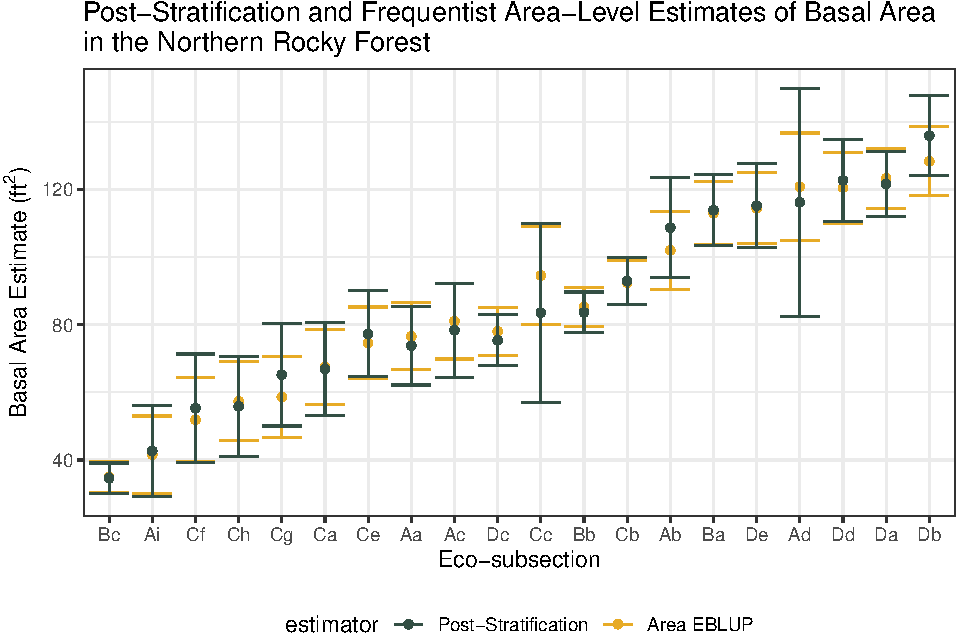
\includegraphics{thesis_files/figure-latex/unnamed-chunk-14-1} 

}

\caption[Coefficient of variation map]{Average log coefficient of variation of each estimator in each eco-subsection plotted onto a map of the Interior West. The average is taken over the four response variables. The natural log is used to perserve a reasonable color scale. Grey areas represent areas where models were not fit.}\label{fig:unnamed-chunk-14}
\end{figure}
We see that the three estimators which have coefficient of variation values higher than one generally produce these values in heavily deserted areas in the southern parts of the Interior West and some deserts in the north parts of Nevada. It is sensible that these areas may truly have low values for our response variables given that the post-stratified estimator is doing its job correctly and the population totals for forested and non-forested areas are correct. On the other hand, it may be reasonable to use a higher variance estimate in these cases and borrow strength from surrounding areas. While it is hard to say which approach to handling these situations gives a better estimate, it highlights distinct ways in which the hierarchical Bayesian estimators (and the unit-level EBLUP) perform differently than the direct estimators and area-level EBLUP. When examining the Northern Rocky Forest we notice the behavior of the hierarchical Bayesian area-level estimator ``pulling up'' lower valued eco-subsections compared to their post-stratified estimate:
\begin{figure}

{\centering 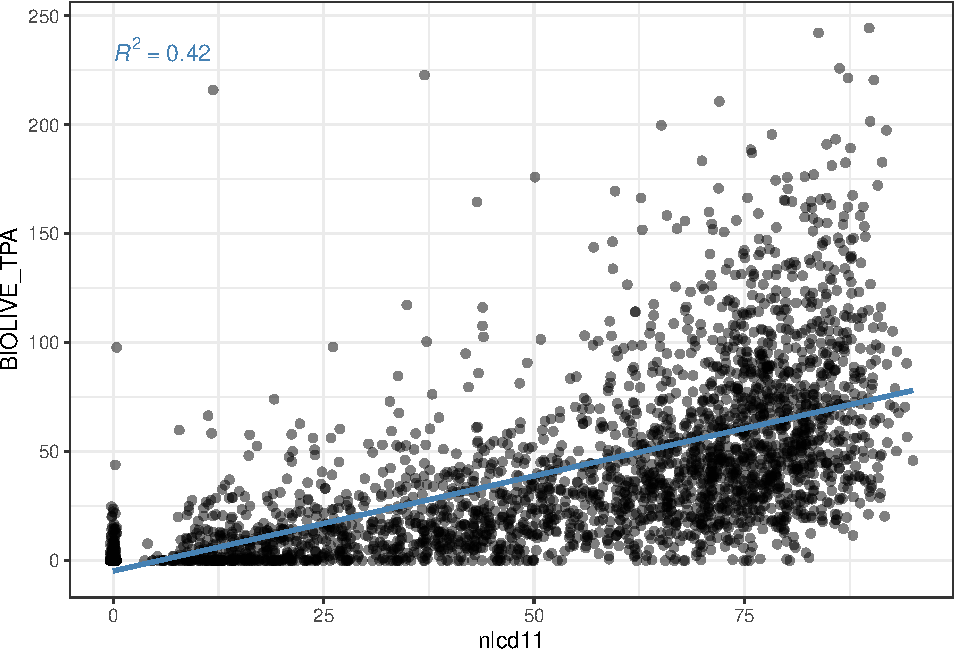
\includegraphics[width=1\linewidth]{thesis_files/figure-latex/unnamed-chunk-15-1} 

}

\caption[HB Area and Post-stratified estimates in M333]{The hierarchical Bayesian area-level estimator and post-stratified estimator predicting basal area in the Northern Rocky Forest.}\label{fig:unnamed-chunk-15}
\end{figure}
We also observe that the eco-subsections with high response values will get ``pulled down'', however the coefficient of variation does not increase significantly here as the sample mean is still relatively high. The ``pulling up'' and ``pushing down'' of estimates is a trait expected of these hierarchical Bayesian models, and it is the realization of ``borrowing strength'' or ``pooling information'' (McElreath, 2020).

The frequentist area-level estimator takes a different approach to making these estimates. Notably, in the case of small within-area variation we see that the EBLUP will put a heavy weight on the post-stratified estimate from Equation \eqref{eq:eblup-area-weight}. We can see this occur by comparing the area-level frequentist estimator to the post-stratified estimate with the same eco-province and response variable as above:
\begin{figure}

{\centering 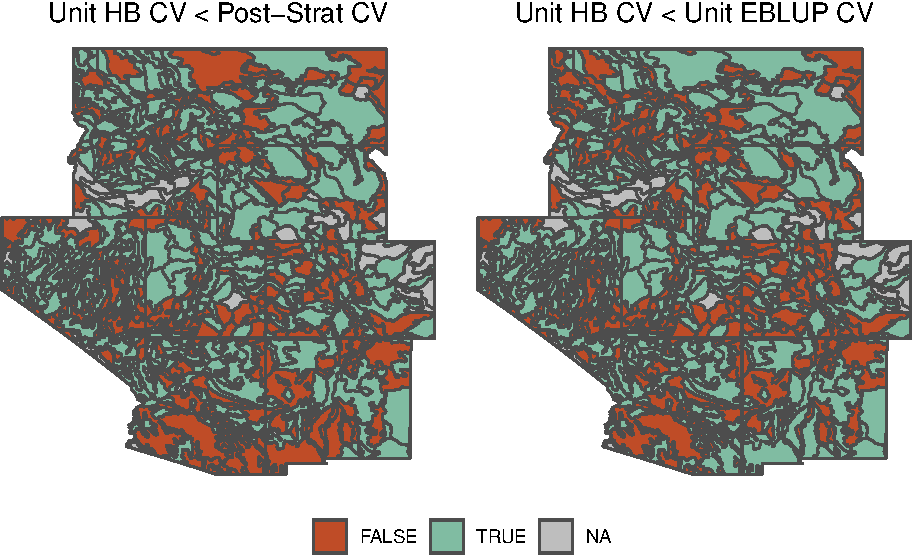
\includegraphics[width=1\linewidth]{thesis_files/figure-latex/unnamed-chunk-16-1} 

}

\caption[EBLUP area-level and Post-stratified estimates in M333]{The frequentist area-level estimator and post-stratified estimator predicting basal area in the Northern Rocky Forest.}\label{fig:unnamed-chunk-16}
\end{figure}
Overall, we can see that the frequentist area-level estimator performs much more similarly to the post-stratified estimator, a trait that may or may not be appealing based on the confidence we have in representative sampling. However, it is important to note that the frequentist area-level estimator is still borrowing strength, it just seems that it will often borrow less strength than the hierarchical Bayesian area-level estimator.

While it is visualally insightful to compare these estimators in the Northern Rocky Forest, it is also beneficial to looking at the numbers across the Interior West. In an attempt to quantify the magnitude of difference between two estimators we introduce percent relative difference, which we define below.
\begin{align*}
PRD(\hat\mu_1,~ \hat\mu_2) = \frac{\hat \mu_1 - \hat\mu_2}{\hat\mu_2} \cdot 100
\end{align*}
While we could explore percent relative difference between all combinations of estimators, the Forest Inventory and Analysis Program's go-to estimator is post-stratification, so we will compare the remaining five estimators to post-stratification. Below, we can see the quantiles of percent relative difference to post-stratification.
\begin{longtable}[t]{lrrrrr}
\caption{\label{tab:unnamed-chunk-17}Quantiles of Percent Relative Difference to the Post-Stratified Estimator}\\
\toprule
Estimator & 0\% & 25\% & 50\% & 75\% & 100\%\\
\midrule
Unit HB & -99.928 & 1.326 & 21.816 & 94.770 & 24224.087\\
Area HB & -74.491 & -13.192 & 13.095 & 66.254 & 105994.261\\
Unit EBLUP & -80.319 & 3.521 & 25.471 & 99.885 & 27724.471\\
Area EBLUP & -79.641 & -3.747 & -0.165 & 2.802 & 160.843\\
\bottomrule
\end{longtable}
These quantiles continue to enforce the idea that the area-level EBLUP generally performs very similarly to the post-stratified estimator (albeit with lower variance). Notably though, the percent relative difference between the area-level hierarchical Bayesian estimator and the post-stratified estimator is small compared to both unit-level models. Percent relative difference to the post-stratified estimator can be thought of in some senses as a weak proxy for bias. However, this is a difficult comparison to make when we do not have the parameter values. While this proxy for bias may be weak, it is reassuring that for the area-level hierarchical Bayesian estimator our median (50\% quantile) percent relative difference is somewhat low.
\begin{center}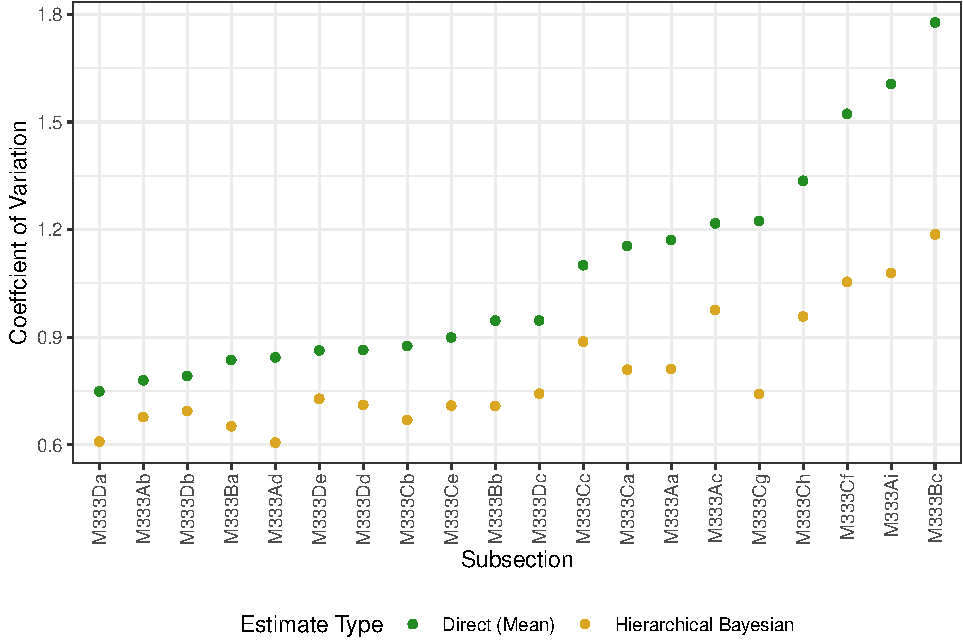
\includegraphics{thesis_files/figure-latex/unnamed-chunk-18-1} \end{center}
\begin{center}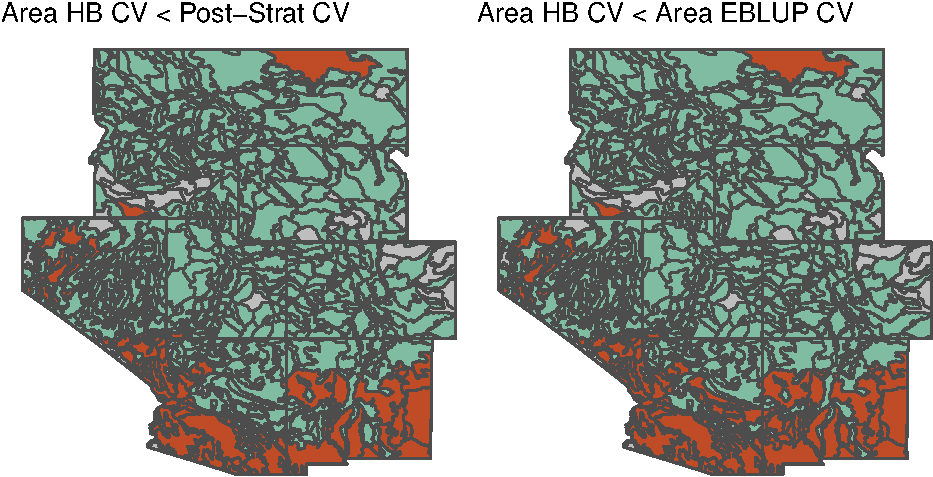
\includegraphics{thesis_files/figure-latex/unnamed-chunk-18-2} \end{center}

The Northern Rocky Forest is a large eco-province spanning many states, and can be seen in Figure \ref{fig:northern-rocky}.

\hypertarget{discussion-and-conclusion}{%
\chapter{Discussion and Conclusion}\label{discussion-and-conclusion}}

If we don't want Conclusion to have a chapter number next to it, we can add the \texttt{\{-\}} attribute.

\textbf{More info}

And here's some other random info: the first paragraph after a chapter title or section head \emph{shouldn't be} indented, because indents are to tell the reader that you're starting a new paragraph. Since that's obvious after a chapter or section title, proper typesetting doesn't add an indent there.

\appendix

\hypertarget{code-appendix}{%
\chapter{Code Appendix}\label{code-appendix}}

This appendix includes the code used to create the estimates used in this thesis. We include both the helper functions created to run the analyses and the implementation of these helper functions.

\hypertarget{helper-functions}{%
\section{Helper Functions}\label{helper-functions}}

\hypertarget{the-sample-mean}{%
\subsection{The Sample Mean}\label{the-sample-mean}}
\begin{Shaded}
\begin{Highlighting}[]
\NormalTok{direct_estimate <-}\StringTok{ }\ControlFlowTok{function}\NormalTok{(data, response, small_area) \{}
  \CommentTok{# Load packages}
  \KeywordTok{library}\NormalTok{(sae)}
  
  \CommentTok{# Create dataframe}
\NormalTok{  dat <-}\StringTok{ }\KeywordTok{data.frame}\NormalTok{(}
    \DataTypeTok{y =}\NormalTok{ data[[response]],}
    \DataTypeTok{small_area =}\NormalTok{ data[[small_area]]}
\NormalTok{  )}
  
  \CommentTok{# Compute estimate}
\NormalTok{  sae}\OperatorTok{::}\KeywordTok{direct}\NormalTok{(}\DataTypeTok{y =}\NormalTok{ dat}\OperatorTok{$}\NormalTok{y,}
              \DataTypeTok{dom =}\NormalTok{ dat}\OperatorTok{$}\NormalTok{small_area,}
              \DataTypeTok{replace =} \OtherTok{TRUE}\NormalTok{)}
\NormalTok{\}}
\end{Highlighting}
\end{Shaded}
\hypertarget{post-stratification}{%
\subsection{Post-Stratification}\label{post-stratification}}
\begin{Shaded}
\begin{Highlighting}[]
\NormalTok{postStrat2_bio <-}\StringTok{ }\ControlFlowTok{function}\NormalTok{(data, strata) \{}
\NormalTok{  est <-}\StringTok{ }\NormalTok{mase}\OperatorTok{::}\KeywordTok{postStrat}\NormalTok{(}\DataTypeTok{y =}\NormalTok{ data[[}\StringTok{"BIOLIVE_TPA"}\NormalTok{]],}
                  \DataTypeTok{x_sample =}\NormalTok{ data[[}\StringTok{"FIAstrat"}\NormalTok{]],}
                  \DataTypeTok{x_pop =}\NormalTok{ strata,}
                  \DataTypeTok{data_type =} \StringTok{"totals"}\NormalTok{,}
                  \DataTypeTok{var_est =}\NormalTok{ T)}
  \KeywordTok{return}\NormalTok{(}\KeywordTok{data.frame}\NormalTok{(}\DataTypeTok{ps_est =}\NormalTok{ est}\OperatorTok{$}\NormalTok{pop_mean,}
                    \DataTypeTok{sd =} \KeywordTok{sqrt}\NormalTok{(est}\OperatorTok{$}\NormalTok{pop_mean_var)))}
\NormalTok{\}}
\NormalTok{postStrat2_ba <-}\StringTok{ }\ControlFlowTok{function}\NormalTok{(data, strata) \{}
\NormalTok{  est <-}\StringTok{ }\NormalTok{mase}\OperatorTok{::}\KeywordTok{postStrat}\NormalTok{(}\DataTypeTok{y =}\NormalTok{ data[[}\StringTok{"BALIVE_TPA"}\NormalTok{]],}
                  \DataTypeTok{x_sample =}\NormalTok{ data[[}\StringTok{"FIAstrat"}\NormalTok{]],}
                  \DataTypeTok{x_pop =}\NormalTok{ strata,}
                  \DataTypeTok{data_type =} \StringTok{"totals"}\NormalTok{,}
                  \DataTypeTok{var_est =}\NormalTok{ T)}
  \KeywordTok{return}\NormalTok{(}\KeywordTok{data.frame}\NormalTok{(}\DataTypeTok{ps_est =}\NormalTok{ est}\OperatorTok{$}\NormalTok{pop_mean,}
                    \DataTypeTok{sd =} \KeywordTok{sqrt}\NormalTok{(est}\OperatorTok{$}\NormalTok{pop_mean_var)))}
\NormalTok{\}}

\NormalTok{postStrat2_voln <-}\StringTok{ }\ControlFlowTok{function}\NormalTok{(data, strata) \{}
\NormalTok{  est <-}\StringTok{ }\NormalTok{mase}\OperatorTok{::}\KeywordTok{postStrat}\NormalTok{(}\DataTypeTok{y =}\NormalTok{ data[[}\StringTok{"VOLNLIVE_TPA"}\NormalTok{]],}
                  \DataTypeTok{x_sample =}\NormalTok{ data[[}\StringTok{"FIAstrat"}\NormalTok{]],}
                  \DataTypeTok{x_pop =}\NormalTok{ strata,}
                  \DataTypeTok{data_type =} \StringTok{"totals"}\NormalTok{,}
                  \DataTypeTok{var_est =}\NormalTok{ T)}
  \KeywordTok{return}\NormalTok{(}\KeywordTok{data.frame}\NormalTok{(}\DataTypeTok{ps_est =}\NormalTok{ est}\OperatorTok{$}\NormalTok{pop_mean,}
                    \DataTypeTok{sd =} \KeywordTok{sqrt}\NormalTok{(est}\OperatorTok{$}\NormalTok{pop_mean_var)))}
\NormalTok{\}}

\NormalTok{postStrat2_cnt <-}\StringTok{ }\ControlFlowTok{function}\NormalTok{(data, strata) \{}
\NormalTok{  est <-}\StringTok{ }\NormalTok{mase}\OperatorTok{::}\KeywordTok{postStrat}\NormalTok{(}\DataTypeTok{y =}\NormalTok{ data[[}\StringTok{"CNTLIVE_TPA"}\NormalTok{]],}
                  \DataTypeTok{x_sample =}\NormalTok{ data[[}\StringTok{"FIAstrat"}\NormalTok{]],}
                  \DataTypeTok{x_pop =}\NormalTok{ strata,}
                  \DataTypeTok{data_type =} \StringTok{"totals"}\NormalTok{,}
                  \DataTypeTok{var_est =}\NormalTok{ T)}
  \KeywordTok{return}\NormalTok{(}\KeywordTok{data.frame}\NormalTok{(}\DataTypeTok{ps_est =}\NormalTok{ est}\OperatorTok{$}\NormalTok{pop_mean,}
                    \DataTypeTok{sd =} \KeywordTok{sqrt}\NormalTok{(est}\OperatorTok{$}\NormalTok{pop_mean_var)))}
\NormalTok{\}}
\end{Highlighting}
\end{Shaded}
\hypertarget{hierarchical-bayesian-unit-level}{%
\subsection{Hierarchical Bayesian Unit-Level}\label{hierarchical-bayesian-unit-level}}
\begin{Shaded}
\begin{Highlighting}[]
\NormalTok{hb_unit <-}\StringTok{ }\ControlFlowTok{function}\NormalTok{(data, formula, small_area, pop_data) \{}
  \CommentTok{# Load packages}
  \KeywordTok{library}\NormalTok{(tidyverse)}
  \KeywordTok{library}\NormalTok{(hbsae)}
  
  \CommentTok{# Create model frame}
\NormalTok{  model_frame <-}\StringTok{ }\KeywordTok{model.frame}\NormalTok{(formula, data) }\OperatorTok
\StringTok{    }\NormalTok{dplyr}\OperatorTok{::}\KeywordTok{mutate}\NormalTok{(}\DataTypeTok{small_area =}\NormalTok{ data[[small_area]])}
  \KeywordTok{colnames}\NormalTok{(model_frame) <-}\StringTok{ }\KeywordTok{c}\NormalTok{(}\StringTok{"y"}\NormalTok{, }\StringTok{"x"}\NormalTok{, }\StringTok{"small_area"}\NormalTok{)}
  
  \CommentTok{# Area population sizes}
\NormalTok{  pop_size <-}\StringTok{ }\NormalTok{pop_data }\OperatorTok
\StringTok{    }\NormalTok{dplyr}\OperatorTok{::}\KeywordTok{filter}\NormalTok{(zoneid }\OperatorTok\StringTok{ }\NormalTok{model_frame}\OperatorTok{$}\NormalTok{small_area) }\OperatorTok
\StringTok{    }\NormalTok{dplyr}\OperatorTok{::}\KeywordTok{select}\NormalTok{(zoneid, sum) }\OperatorTok
\StringTok{    }\NormalTok{dplyr}\OperatorTok{::}\KeywordTok{rename}\NormalTok{(}\DataTypeTok{pop_size =}\NormalTok{ sum) }\OperatorTok
\StringTok{    }\NormalTok{dplyr}\OperatorTok{::}\KeywordTok{select}\NormalTok{(pop_size)}
  
  \CommentTok{# Create population means matrix}
\NormalTok{  pop_means <-}\StringTok{ }\NormalTok{pop_data }\OperatorTok
\StringTok{    }\NormalTok{dplyr}\OperatorTok{::}\KeywordTok{filter}\NormalTok{(zoneid }\OperatorTok\StringTok{ }\NormalTok{model_frame}\OperatorTok{$}\NormalTok{small_area) }\OperatorTok
\StringTok{    }\NormalTok{dplyr}\OperatorTok{::}\KeywordTok{select}\NormalTok{(zoneid, mean) }\OperatorTok
\StringTok{    }\NormalTok{dplyr}\OperatorTok{::}\KeywordTok{rename}\NormalTok{(}\DataTypeTok{x =}\NormalTok{ mean) }\OperatorTok
\StringTok{    }\KeywordTok{column_to_rownames}\NormalTok{(}\StringTok{"zoneid"}\NormalTok{)}
  
  \CommentTok{# Create lambda}
\NormalTok{  anova <-}\StringTok{ }\KeywordTok{aov}\NormalTok{(y }\OperatorTok{~}\StringTok{ }\NormalTok{small_area, }\DataTypeTok{data =}\NormalTok{ model_frame)}
\NormalTok{  l <-}\StringTok{ }\KeywordTok{summary}\NormalTok{(anova)[[}\DecValTok{1}\NormalTok{]][}\StringTok{"small_area"}\NormalTok{, }\StringTok{"F value"}\NormalTok{]}
  
  \CommentTok{# Fit the model}
\NormalTok{  mod <-}\StringTok{ }\KeywordTok{fSAE.Unit}\NormalTok{(}
    \DataTypeTok{y =} \KeywordTok{model.frame}\NormalTok{(formula, }\DataTypeTok{data =}\NormalTok{ data)[, }\DecValTok{1}\NormalTok{],}
    \DataTypeTok{X =} \KeywordTok{data.frame}\NormalTok{(}\DataTypeTok{X =} \KeywordTok{model.frame}\NormalTok{(formula, }\DataTypeTok{data =}\NormalTok{ data)[,}\OperatorTok{-}\DecValTok{1}\NormalTok{]),}
    \DataTypeTok{area =}\NormalTok{ data[[small_area]],}
    \DataTypeTok{Narea =}\NormalTok{ pop_size}\OperatorTok{$}\NormalTok{pop_size,}
    \DataTypeTok{Xpop =}\NormalTok{ pop_means,}
    \DataTypeTok{fpc =} \OtherTok{TRUE}\NormalTok{,}
    \DataTypeTok{lambda0 =}\NormalTok{ l,}
    \DataTypeTok{silent =}\NormalTok{ T}
\NormalTok{  )}

  \CommentTok{# Calculate CoV}
\NormalTok{  mean_y <-}\StringTok{ }\NormalTok{model_frame }\OperatorTok
\StringTok{    }\NormalTok{dplyr}\OperatorTok{::}\KeywordTok{group_by}\NormalTok{(small_area) }\OperatorTok
\StringTok{    }\NormalTok{dplyr}\OperatorTok{::}\KeywordTok{summarise}\NormalTok{(}\DataTypeTok{mean_y =} \KeywordTok{mean}\NormalTok{(y))}
\NormalTok{  CoV <-}\StringTok{ }\NormalTok{hbsae}\OperatorTok{::}\KeywordTok{SE}\NormalTok{(mod) }\OperatorTok{/}\StringTok{ }\NormalTok{mean_y}\OperatorTok{$}\NormalTok{mean_y}

  \CommentTok{## Add to model object}
\NormalTok{  mod}\OperatorTok{$}\NormalTok{CoV <-}\StringTok{ }\NormalTok{CoV}

  \CommentTok{# Print model}
\NormalTok{  mod}
\NormalTok{\}}
\end{Highlighting}
\end{Shaded}
\hypertarget{hierarchical-bayesian-area-level}{%
\subsection{Hierarchical Bayesian Area-Level}\label{hierarchical-bayesian-area-level}}
\begin{Shaded}
\begin{Highlighting}[]
\NormalTok{hb_area <-}\StringTok{ }\ControlFlowTok{function}\NormalTok{(data, formula, small_area,}
\NormalTok{                    pop_data, post_strat_data) \{}
  \CommentTok{# Load packages}
  \KeywordTok{library}\NormalTok{(tidyverse)}
  \KeywordTok{library}\NormalTok{(hbsae)}
  
  \CommentTok{# Create unnamed model frame (to call correct y var in a filter)}
\NormalTok{  mf <-}\StringTok{ }\KeywordTok{model.frame}\NormalTok{(formula, data)}
  
  \CommentTok{# Create model frame}
\NormalTok{  model_frame <-}\StringTok{ }\KeywordTok{model.frame}\NormalTok{(formula, data) }\OperatorTok
\StringTok{    }\NormalTok{dplyr}\OperatorTok{::}\KeywordTok{mutate}\NormalTok{(}\DataTypeTok{small_area =}\NormalTok{ data[[small_area]])}
  \KeywordTok{colnames}\NormalTok{(model_frame) <-}\StringTok{ }\KeywordTok{c}\NormalTok{(}\StringTok{"y"}\NormalTok{, }\StringTok{"x"}\NormalTok{, }\StringTok{"small_area"}\NormalTok{)}
  
  \CommentTok{# Direct X}
\NormalTok{  X <-}\StringTok{ }\NormalTok{pop_data }\OperatorTok
\StringTok{    }\NormalTok{dplyr}\OperatorTok{::}\KeywordTok{filter}\NormalTok{(zoneid }\OperatorTok\StringTok{ }\NormalTok{model_frame}\OperatorTok{$}\NormalTok{small_area) }\OperatorTok
\StringTok{    }\NormalTok{dplyr}\OperatorTok{::}\KeywordTok{select}\NormalTok{(zoneid, mean) }\OperatorTok
\StringTok{    }\NormalTok{dplyr}\OperatorTok{::}\KeywordTok{rename}\NormalTok{(}\DataTypeTok{mean_x =}\NormalTok{ mean,}
                  \DataTypeTok{small_area =}\NormalTok{ zoneid) }\OperatorTok
\StringTok{    }\NormalTok{dplyr}\OperatorTok{::}\KeywordTok{arrange}\NormalTok{(small_area)}

  \CommentTok{# Compute direct estimate}
\NormalTok{  mean <-}\StringTok{ }\KeywordTok{direct_estimate}\NormalTok{(model_frame, }\StringTok{"y"}\NormalTok{, }\StringTok{"small_area"}\NormalTok{) }\OperatorTok
\StringTok{    }\NormalTok{dplyr}\OperatorTok{::}\KeywordTok{mutate}\NormalTok{(}\DataTypeTok{var =}\NormalTok{ SD}\OperatorTok{^}\DecValTok{2}\NormalTok{)}
  
\NormalTok{  dir <-}\StringTok{ }\NormalTok{post_strat_data }\OperatorTok
\StringTok{    }\KeywordTok{filter}\NormalTok{(response }\OperatorTok\StringTok{ }\KeywordTok{colnames}\NormalTok{(mf)[}\DecValTok{1}\NormalTok{],}
\NormalTok{           province }\OperatorTok\StringTok{ }\KeywordTok{unique}\NormalTok{(data}\OperatorTok{$}\NormalTok{province)) }\OperatorTok
\StringTok{    }\KeywordTok{arrange}\NormalTok{(subsection)}
  
  \CommentTok{# Create lambda}
\NormalTok{  anova <-}\StringTok{ }\KeywordTok{aov}\NormalTok{(y }\OperatorTok{~}\StringTok{ }\NormalTok{small_area, }\DataTypeTok{data =}\NormalTok{ model_frame)}
\NormalTok{  l <-}\StringTok{ }\KeywordTok{summary}\NormalTok{(anova)[[}\DecValTok{1}\NormalTok{]][}\StringTok{"small_area"}\NormalTok{, }\StringTok{"F value"}\NormalTok{]}

  \CommentTok{# Fit the model}
\NormalTok{  mod <-}\StringTok{ }\KeywordTok{fSAE.Area}\NormalTok{(}
    \DataTypeTok{est.init =}\NormalTok{ dir}\OperatorTok{$}\NormalTok{est,}
    \DataTypeTok{var.init =}\NormalTok{ dir}\OperatorTok{$}\NormalTok{var,}
    \DataTypeTok{X =}\NormalTok{ X }\OperatorTok\StringTok{ }\NormalTok{dplyr}\OperatorTok{::}\KeywordTok{select}\NormalTok{(mean_x),}
    \DataTypeTok{lambda0 =}\NormalTok{ l}
\NormalTok{  )}

  \CommentTok{# Calculate CoV}
\NormalTok{   CoV <-}\StringTok{ }\NormalTok{hbsae}\OperatorTok{::}\KeywordTok{SE}\NormalTok{(mod) }\OperatorTok{/}\StringTok{ }\NormalTok{mean}\OperatorTok{$}\NormalTok{Direct}
\NormalTok{   mod}\OperatorTok{$}\NormalTok{CoV <-}\StringTok{ }\NormalTok{CoV}

  \CommentTok{# Print model}
\NormalTok{  mod}
\NormalTok{\}}
\end{Highlighting}
\end{Shaded}
\hypertarget{frequentist-unit-level}{%
\subsection{Frequentist Unit-Level}\label{frequentist-unit-level}}
\begin{Shaded}
\begin{Highlighting}[]
\NormalTok{freq_unit <-}\StringTok{ }\ControlFlowTok{function}\NormalTok{(data, formula, small_area, pop_data) \{}
  \CommentTok{# Load packages}
  \KeywordTok{library}\NormalTok{(tidyverse)}
  \KeywordTok{library}\NormalTok{(sae)}
  
  \CommentTok{# Create model frame}
\NormalTok{  model_frame <-}\StringTok{ }\KeywordTok{model.frame}\NormalTok{(formula, data) }\OperatorTok
\StringTok{    }\NormalTok{dplyr}\OperatorTok{::}\KeywordTok{mutate}\NormalTok{(}\DataTypeTok{small_area =}\NormalTok{ data[[small_area]])}
  \KeywordTok{colnames}\NormalTok{(model_frame) <-}\StringTok{ }\KeywordTok{c}\NormalTok{(}\StringTok{"y"}\NormalTok{, }\StringTok{"x"}\NormalTok{, }\StringTok{"small_area"}\NormalTok{)}
  
  \CommentTok{# Area population sizes}
\NormalTok{  pop_size <-}\StringTok{ }\NormalTok{pop_data }\OperatorTok
\StringTok{    }\NormalTok{dplyr}\OperatorTok{::}\KeywordTok{filter}\NormalTok{(zoneid }\OperatorTok\StringTok{ }\NormalTok{model_frame}\OperatorTok{$}\NormalTok{small_area) }\OperatorTok
\StringTok{    }\NormalTok{dplyr}\OperatorTok{::}\KeywordTok{select}\NormalTok{(zoneid, sum) }\OperatorTok
\StringTok{    }\NormalTok{dplyr}\OperatorTok{::}\KeywordTok{rename}\NormalTok{(}\DataTypeTok{pop_size =}\NormalTok{ sum,}
                  \DataTypeTok{small_area =}\NormalTok{ zoneid)}
  
  \CommentTok{# Create population means matrix}
\NormalTok{  meanxpop <-}\StringTok{ }\NormalTok{pop_data }\OperatorTok
\StringTok{    }\NormalTok{dplyr}\OperatorTok{::}\KeywordTok{filter}\NormalTok{(zoneid }\OperatorTok\StringTok{ }\NormalTok{model_frame}\OperatorTok{$}\NormalTok{small_area) }\OperatorTok
\StringTok{    }\NormalTok{dplyr}\OperatorTok{::}\KeywordTok{select}\NormalTok{(zoneid, mean) }\OperatorTok
\StringTok{    }\NormalTok{dplyr}\OperatorTok{::}\KeywordTok{rename}\NormalTok{(}\DataTypeTok{x =}\NormalTok{ mean,}
                  \DataTypeTok{small_area =}\NormalTok{ zoneid)}
  
  \CommentTok{# Fit the model}
\NormalTok{  mod <-}\StringTok{ }\KeywordTok{eblupBHF}\NormalTok{(}
    \DataTypeTok{formula =}\NormalTok{ model_frame}\OperatorTok{$}\NormalTok{y }\OperatorTok{~}\StringTok{ }\NormalTok{model_frame}\OperatorTok{$}\NormalTok{x,}
    \DataTypeTok{dom =}\NormalTok{ model_frame}\OperatorTok{$}\NormalTok{small_area,}
    \DataTypeTok{meanxpop =}\NormalTok{ meanxpop,}
    \DataTypeTok{popnsize =}\NormalTok{ pop_size}
\NormalTok{  )}
\NormalTok{  mod}
\NormalTok{\}}
\end{Highlighting}
\end{Shaded}
\hypertarget{frequentist-area-level}{%
\subsection{Frequentist Area-Level}\label{frequentist-area-level}}
\begin{Shaded}
\begin{Highlighting}[]
\NormalTok{freq_area <-}\StringTok{ }\ControlFlowTok{function}\NormalTok{(data, formula, small_area,}
\NormalTok{                      pop_data, post_strat_data) \{}
  \CommentTok{# Load packages}
  \KeywordTok{library}\NormalTok{(tidyverse)}
  \KeywordTok{library}\NormalTok{(sae)}
  
  \CommentTok{# Create model frame}
\NormalTok{  model_frame <-}\StringTok{ }\KeywordTok{model.frame}\NormalTok{(formula, data) }\OperatorTok
\StringTok{    }\NormalTok{dplyr}\OperatorTok{::}\KeywordTok{mutate}\NormalTok{(}\DataTypeTok{small_area =}\NormalTok{ data[[small_area]])}
  \KeywordTok{colnames}\NormalTok{(model_frame) <-}\StringTok{ }\KeywordTok{c}\NormalTok{(}\StringTok{"y"}\NormalTok{, }\StringTok{"x"}\NormalTok{, }\StringTok{"small_area"}\NormalTok{)}
\NormalTok{  model_frame}
  
\NormalTok{  mf <-}\StringTok{ }\KeywordTok{model.frame}\NormalTok{(formula, data)}
  
\NormalTok{  dir <-}\StringTok{ }\NormalTok{post_strat_data }\OperatorTok\StringTok{ }
\StringTok{    }\KeywordTok{filter}\NormalTok{(response }\OperatorTok\StringTok{ }\KeywordTok{colnames}\NormalTok{(mf)[}\DecValTok{1}\NormalTok{],}
\NormalTok{           province }\OperatorTok\StringTok{ }\KeywordTok{unique}\NormalTok{(data}\OperatorTok{$}\NormalTok{province)) }\OperatorTok
\StringTok{    }\KeywordTok{arrange}\NormalTok{(subsection)}
  
  \CommentTok{# Direct X}
\NormalTok{  X <-}\StringTok{ }\NormalTok{pop_data }\OperatorTok
\StringTok{    }\NormalTok{dplyr}\OperatorTok{::}\KeywordTok{filter}\NormalTok{(zoneid }\OperatorTok\StringTok{ }\NormalTok{model_frame}\OperatorTok{$}\NormalTok{small_area) }\OperatorTok
\StringTok{    }\NormalTok{dplyr}\OperatorTok{::}\KeywordTok{select}\NormalTok{(zoneid, mean) }\OperatorTok
\StringTok{    }\NormalTok{dplyr}\OperatorTok{::}\KeywordTok{rename}\NormalTok{(}\DataTypeTok{mean_x =}\NormalTok{ mean,}
                  \DataTypeTok{small_area =}\NormalTok{ zoneid) }\OperatorTok
\StringTok{    }\NormalTok{dplyr}\OperatorTok{::}\KeywordTok{arrange}\NormalTok{(small_area)}
  
  \CommentTok{# Join pop and dir}
\NormalTok{  dat <-}\StringTok{ }\NormalTok{dir }\OperatorTok
\StringTok{    }\KeywordTok{left_join}\NormalTok{(X, }\DataTypeTok{by =} \KeywordTok{c}\NormalTok{(}\StringTok{"subsection"}\NormalTok{ =}\StringTok{ "small_area"}\NormalTok{))}

  \CommentTok{# Fit the model}
\NormalTok{  mod <-}\StringTok{ }\NormalTok{sae}\OperatorTok{::}\KeywordTok{mseFH}\NormalTok{(}\DataTypeTok{formula =}\NormalTok{ dat}\OperatorTok{$}\NormalTok{est }\OperatorTok{~}\StringTok{ }\NormalTok{dat}\OperatorTok{$}\NormalTok{mean_x,}
                      \DataTypeTok{vardir =}\NormalTok{ dat}\OperatorTok{$}\NormalTok{var)}
\NormalTok{  mod}
  
\NormalTok{\}}
\end{Highlighting}
\end{Shaded}
\hypertarget{coeffiicent-of-variation-functions}{%
\subsection{Coeffiicent of Variation Functions}\label{coeffiicent-of-variation-functions}}
\begin{Shaded}
\begin{Highlighting}[]
\NormalTok{hb_CoV <-}\StringTok{ }\ControlFlowTok{function}\NormalTok{(data) \{}
  \CommentTok{# Load packages}
  \KeywordTok{library}\NormalTok{(tidyverse)}
  \KeywordTok{library}\NormalTok{(hbsae)}
  
  \CommentTok{# Grab CoV}
\NormalTok{  data}\OperatorTok{$}\NormalTok{CoV}
\NormalTok{\}}

\NormalTok{freq_unit_CoV <-}\StringTok{ }\ControlFlowTok{function}\NormalTok{(data, formula, small_area,}
\NormalTok{                          pop_data, }\DataTypeTok{B =} \DecValTok{100}\NormalTok{) \{}
  \CommentTok{# Load packages}
  \KeywordTok{library}\NormalTok{(tidyverse)}
  \KeywordTok{library}\NormalTok{(sae)}
  
  \CommentTok{# Create empty items for looping}
\NormalTok{  boots <-}\StringTok{ }\KeywordTok{list}\NormalTok{()}
\NormalTok{  fit <-}\StringTok{ }\KeywordTok{list}\NormalTok{()}
\NormalTok{  mean_df <-}\StringTok{ }\KeywordTok{list}\NormalTok{()}
\NormalTok{  final <-}\StringTok{ }\KeywordTok{data.frame}\NormalTok{()}
  
  \CommentTok{# Create model frame}
\NormalTok{  model_frame <-}\StringTok{ }\KeywordTok{model.frame}\NormalTok{(formula, data) }\OperatorTok
\StringTok{    }\NormalTok{dplyr}\OperatorTok{::}\KeywordTok{mutate}\NormalTok{(}\DataTypeTok{small_area =}\NormalTok{ data[[small_area]])}
  \KeywordTok{colnames}\NormalTok{(model_frame) <-}\StringTok{ }\KeywordTok{c}\NormalTok{(}\StringTok{"y"}\NormalTok{, }\StringTok{"x"}\NormalTok{, }\StringTok{"small_area"}\NormalTok{)}
  
  \CommentTok{# Nest by small area}
\NormalTok{  data_nested <-}\StringTok{ }\NormalTok{model_frame }\OperatorTok
\StringTok{    }\KeywordTok{mutate}\NormalTok{(}\DataTypeTok{id =}\NormalTok{ small_area) }\OperatorTok
\StringTok{    }\KeywordTok{group_by}\NormalTok{(small_area) }\OperatorTok
\StringTok{    }\KeywordTok{nest}\NormalTok{()}
  
  \CommentTok{# Bootstrap}
  \ControlFlowTok{for}\NormalTok{(i }\ControlFlowTok{in} \DecValTok{1}\OperatorTok{:}\NormalTok{B)\{}
    \ControlFlowTok{for}\NormalTok{(j }\ControlFlowTok{in} \DecValTok{1}\OperatorTok{:}\KeywordTok{length}\NormalTok{(}\KeywordTok{unique}\NormalTok{(model_frame}\OperatorTok{$}\NormalTok{small_area))) \{}
\NormalTok{      boots[[j]] <-}\StringTok{ }\KeywordTok{sample_n}\NormalTok{(}
\NormalTok{        data_nested[[}\DecValTok{2}\NormalTok{]][[j]],}
        \DataTypeTok{size =} \KeywordTok{length}\NormalTok{(data_nested[[}\DecValTok{2}\NormalTok{]][[j]]}\OperatorTok{$}\NormalTok{y),}
        \DataTypeTok{replace =} \OtherTok{TRUE}
\NormalTok{      )}
\NormalTok{      boots_df <-}\StringTok{ }\KeywordTok{bind_rows}\NormalTok{(boots) }
\NormalTok{    \}}
    
\NormalTok{    fit[[i]] <-}\StringTok{ }\KeywordTok{freq_unit}\NormalTok{(boots_df, y }\OperatorTok{~}\StringTok{ }\NormalTok{x, }\StringTok{"id"}\NormalTok{, pop_data)}
    
\NormalTok{    mean_df[[i]] <-}\StringTok{ }\KeywordTok{data.frame}\NormalTok{(}\DataTypeTok{fitted =}\NormalTok{ fit[[i]]}\OperatorTok{$}\NormalTok{eblup}\OperatorTok{$}\NormalTok{eblup,}
                               \DataTypeTok{subsection =}\NormalTok{ fit[[i]]}\OperatorTok{$}\NormalTok{eblup}\OperatorTok{$}\NormalTok{domain)}
    \ControlFlowTok{if}\NormalTok{ (i }\OperatorTok\StringTok{ }\DecValTok{50} \OperatorTok{==}\StringTok{ }\DecValTok{1}\NormalTok{) \{}
      \KeywordTok{print}\NormalTok{(i)}
\NormalTok{    \}}
\NormalTok{  \}}
  
  \CommentTok{# Create final output}
\NormalTok{  final <-}\StringTok{ }\KeywordTok{bind_rows}\NormalTok{(mean_df) }\OperatorTok
\StringTok{    }\KeywordTok{group_by}\NormalTok{(subsection) }\OperatorTok
\StringTok{    }\KeywordTok{summarize}\NormalTok{(}\DataTypeTok{sd =} \KeywordTok{sd}\NormalTok{(fitted, }\DataTypeTok{na.rm =} \OtherTok{TRUE}\NormalTok{))}
\NormalTok{  mean_y <-}\StringTok{ }\NormalTok{model_frame }\OperatorTok
\StringTok{    }\NormalTok{dplyr}\OperatorTok{::}\KeywordTok{group_by}\NormalTok{(small_area) }\OperatorTok
\StringTok{    }\NormalTok{dplyr}\OperatorTok{::}\KeywordTok{summarise}\NormalTok{(}\DataTypeTok{mean_y =} \KeywordTok{mean}\NormalTok{(y, }\DataTypeTok{na.rm =} \OtherTok{TRUE}\NormalTok{))}
  
\NormalTok{  COV <-}\StringTok{ }\NormalTok{final}\OperatorTok{$}\NormalTok{sd }\OperatorTok{/}\StringTok{ }\NormalTok{mean_y}\OperatorTok{$}\NormalTok{mean_y}
  \KeywordTok{names}\NormalTok{(COV) <-}\StringTok{ }\NormalTok{final}\OperatorTok{$}\NormalTok{subsection}
  
\NormalTok{  COV}
\NormalTok{\}}
\end{Highlighting}
\end{Shaded}
\hypertarget{fitting-models}{%
\section{Fitting Models}\label{fitting-models}}

\hypertarget{data-set-up-preprocessing}{%
\subsection{Data Set-up \& Preprocessing}\label{data-set-up-preprocessing}}
\begin{Shaded}
\begin{Highlighting}[]
\KeywordTok{library}\NormalTok{(tidyverse)}
\KeywordTok{library}\NormalTok{(mase)}
\KeywordTok{library}\NormalTok{(hbsae)}
\KeywordTok{library}\NormalTok{(sae)}
\end{Highlighting}
\end{Shaded}
\begin{Shaded}
\begin{Highlighting}[]
\NormalTok{intwest <-}\StringTok{ }\KeywordTok{read_csv}\NormalTok{(}\StringTok{"data/subsets/df.csv"}\NormalTok{)}
\NormalTok{tccpop <-}\StringTok{ }\KeywordTok{read_csv}\NormalTok{(}\StringTok{"data/population/tcc_pop.csv"}\NormalTok{)}
\NormalTok{strata <-}\StringTok{ }\KeywordTok{read_csv}\NormalTok{(}\StringTok{"data/population/strata.csv"}\NormalTok{)}
\end{Highlighting}
\end{Shaded}
\begin{Shaded}
\begin{Highlighting}[]
\CommentTok{# Set-up strata:}
\NormalTok{intwest <-}\StringTok{ }\NormalTok{intwest }\OperatorTok
\StringTok{  }\KeywordTok{mutate}\NormalTok{(}\DataTypeTok{FIAstrat =} \KeywordTok{case_when}\NormalTok{(}
\NormalTok{    FIAstrat }\OperatorTok{==}\StringTok{ "1"} \OperatorTok{~}\StringTok{ "Sampled-Forest"}\NormalTok{,}
\NormalTok{    FIAstrat }\OperatorTok{==}\StringTok{ "2"} \OperatorTok{~}\StringTok{ "Sampled-Nonforest"}\NormalTok{,}
\NormalTok{    FIAstrat }\OperatorTok{==}\StringTok{ "0"} \OperatorTok{~}\StringTok{ "Sampled-Nonforest"}\NormalTok{,}
\NormalTok{    FIAstrat }\OperatorTok{==}\StringTok{ "3"} \OperatorTok{~}\StringTok{ "Sampled-Nonforest"}\NormalTok{,}
\NormalTok{  )) }
\end{Highlighting}
\end{Shaded}
\begin{Shaded}
\begin{Highlighting}[]
\CommentTok{# Filter out subsections that cause errors in computation}
\NormalTok{no0_subsections <-}\StringTok{ }\NormalTok{intwest }\OperatorTok
\StringTok{  }\KeywordTok{group_by}\NormalTok{(subsection) }\OperatorTok
\StringTok{  }\KeywordTok{summarize}\NormalTok{(}\DataTypeTok{mean_y =} \KeywordTok{mean}\NormalTok{(BIOLIVE_TPA),}
            \DataTypeTok{mean_x =} \KeywordTok{mean}\NormalTok{(nlcd11)) }\OperatorTok
\StringTok{  }\KeywordTok{filter}\NormalTok{(mean_y }\OperatorTok{>}\StringTok{ }\DecValTok{0} \OperatorTok{&}\StringTok{ }\NormalTok{mean_x }\OperatorTok{>}\StringTok{ }\DecValTok{0}\NormalTok{) }\OperatorTok\StringTok{ }
\StringTok{  }\NormalTok{dplyr}\OperatorTok{::}\KeywordTok{select}\NormalTok{(subsection) }\OperatorTok
\StringTok{  }\KeywordTok{pull}\NormalTok{()}

\NormalTok{intwest_no0 <-}\StringTok{ }\NormalTok{intwest }\OperatorTok
\StringTok{  }\KeywordTok{filter}\NormalTok{(subsection }\OperatorTok\StringTok{ }\NormalTok{no0_subsections) }\OperatorTok
\StringTok{  }\KeywordTok{filter}\NormalTok{(}\OperatorTok{!}\NormalTok{(province }\OperatorTok\StringTok{ }\KeywordTok{c}\NormalTok{(}\StringTok{"M261"}\NormalTok{, }\StringTok{"M334"}\NormalTok{))) }\OperatorTok\StringTok{ }
\StringTok{  }\KeywordTok{filter}\NormalTok{(}\OperatorTok{!}\NormalTok{(subsection }\OperatorTok\StringTok{ }\KeywordTok{c}\NormalTok{(}\StringTok{"342Fi"}\NormalTok{, }\StringTok{"331Kj"}\NormalTok{, }\StringTok{"342Dh"}\NormalTok{, }\StringTok{"341Dc"}\NormalTok{))) }
\end{Highlighting}
\end{Shaded}
\begin{Shaded}
\begin{Highlighting}[]
\CommentTok{# Create list of dataframes}
\NormalTok{iw <-}\StringTok{ }\KeywordTok{split}\NormalTok{(intwest_no0, }\DataTypeTok{f =}\NormalTok{ intwest_no0}\OperatorTok{$}\NormalTok{province)}
\end{Highlighting}
\end{Shaded}
\hypertarget{direct-estimation-1}{%
\subsection{Direct Estimation}\label{direct-estimation-1}}
\begin{Shaded}
\begin{Highlighting}[]
\NormalTok{strata <-}\StringTok{ }\NormalTok{strata }\OperatorTok
\StringTok{  }\KeywordTok{filter}\NormalTok{(zoneid }\OperatorTok\StringTok{ }\KeywordTok{unique}\NormalTok{(intwest_no0}\OperatorTok{$}\NormalTok{subsection)) }\OperatorTok
\StringTok{  }\KeywordTok{mutate}\NormalTok{(}
    \DataTypeTok{fnf_no_water =} \KeywordTok{case_when}\NormalTok{(}
\NormalTok{      fnf_no_water }\OperatorTok{==}\StringTok{ }\DecValTok{1} \OperatorTok{~}\StringTok{ "Sampled-Forest"}\NormalTok{,}
\NormalTok{      fnf_no_water }\OperatorTok{==}\StringTok{ }\DecValTok{2} \OperatorTok{~}\StringTok{ "Sampled-Nonforest"}
\NormalTok{    )}
\NormalTok{  )}
\NormalTok{strata <-}\StringTok{ }\NormalTok{strata }\OperatorTok
\StringTok{  }\NormalTok{dplyr}\OperatorTok{::}\KeywordTok{select}\NormalTok{(}\OperatorTok{-}\NormalTok{zoneprop)}

\CommentTok{# split strata into list and drop column split by}
\NormalTok{strata_list <-}\StringTok{ }\KeywordTok{lapply}\NormalTok{(}
  \KeywordTok{split}\NormalTok{(strata, }\DataTypeTok{f =}\NormalTok{ strata}\OperatorTok{$}\NormalTok{zoneid),}
  \ControlFlowTok{function}\NormalTok{(strata) \{ strata}\OperatorTok{$}\NormalTok{zoneid <-}\StringTok{ }\OtherTok{NULL}\NormalTok{; strata\}}
\NormalTok{  )}

\CommentTok{# split subsections into list}
\NormalTok{subsection_list <-}\StringTok{ }\KeywordTok{split}\NormalTok{(intwest_no0,}
\NormalTok{                         intwest_no0}\OperatorTok{$}\NormalTok{subsection)}


\NormalTok{post_strat_bio <-}\StringTok{ }\KeywordTok{map2}\NormalTok{(}\DataTypeTok{.x =}\NormalTok{ subsection_list,}
                       \DataTypeTok{.y =}\NormalTok{ strata_list,}
                       \DataTypeTok{.f =}\NormalTok{ postStrat2_bio)}
\NormalTok{post_strat_ba <-}\StringTok{ }\KeywordTok{map2}\NormalTok{(}\DataTypeTok{.x =}\NormalTok{ subsection_list,}
                      \DataTypeTok{.y =}\NormalTok{ strata_list,}
                      \DataTypeTok{.f =}\NormalTok{ postStrat2_ba)}
\NormalTok{post_strat_voln <-}\StringTok{ }\KeywordTok{map2}\NormalTok{(}\DataTypeTok{.x =}\NormalTok{ subsection_list,}
                        \DataTypeTok{.y =}\NormalTok{ strata_list,}
                        \DataTypeTok{.f =}\NormalTok{ postStrat2_voln)}
\NormalTok{post_strat_cnt <-}\StringTok{ }\KeywordTok{map2}\NormalTok{(}\DataTypeTok{.x =}\NormalTok{ subsection_list,}
                       \DataTypeTok{.y =}\NormalTok{ strata_list,}
                       \DataTypeTok{.f =}\NormalTok{ postStrat2_cnt)}

\NormalTok{results <-}\StringTok{ }\KeywordTok{data.frame}\NormalTok{(}
  \DataTypeTok{ps_est =} \KeywordTok{c}\NormalTok{(}\KeywordTok{bind_rows}\NormalTok{(post_strat_bio)}\OperatorTok{$}\NormalTok{ps_est,}
             \KeywordTok{bind_rows}\NormalTok{(post_strat_ba)}\OperatorTok{$}\NormalTok{ps_est,}
             \KeywordTok{bind_rows}\NormalTok{(post_strat_cnt)}\OperatorTok{$}\NormalTok{ps_est,}
             \KeywordTok{bind_rows}\NormalTok{(post_strat_voln)}\OperatorTok{$}\NormalTok{ps_est),}
  \DataTypeTok{ps_sd =} \KeywordTok{c}\NormalTok{(}\KeywordTok{bind_rows}\NormalTok{(post_strat_bio)}\OperatorTok{$}\NormalTok{sd,}
             \KeywordTok{bind_rows}\NormalTok{(post_strat_ba)}\OperatorTok{$}\NormalTok{sd,}
             \KeywordTok{bind_rows}\NormalTok{(post_strat_cnt)}\OperatorTok{$}\NormalTok{sd,}
             \KeywordTok{bind_rows}\NormalTok{(post_strat_voln)}\OperatorTok{$}\NormalTok{sd),}
  \DataTypeTok{subsection =} \KeywordTok{rep}\NormalTok{(}\KeywordTok{names}\NormalTok{(post_strat_bio), }\DecValTok{4}\NormalTok{),}
  \DataTypeTok{response =} \KeywordTok{c}\NormalTok{(}
    \KeywordTok{rep}\NormalTok{(}\StringTok{"BIOLIVE_TPA"}\NormalTok{, }\KeywordTok{length}\NormalTok{(post_strat_bio)),}
    \KeywordTok{rep}\NormalTok{(}\StringTok{"BALIVE_TPA"}\NormalTok{, }\KeywordTok{length}\NormalTok{(post_strat_ba)),}
    \KeywordTok{rep}\NormalTok{(}\StringTok{"CNTLIVE_TPA"}\NormalTok{, }\KeywordTok{length}\NormalTok{(post_strat_cnt)),}
    \KeywordTok{rep}\NormalTok{(}\StringTok{"VOLNLIVE_TPA"}\NormalTok{, }\KeywordTok{length}\NormalTok{(post_strat_voln)))}
\NormalTok{)}
\end{Highlighting}
\end{Shaded}
\begin{Shaded}
\begin{Highlighting}[]
\NormalTok{dirmean <-}\StringTok{ }\KeywordTok{list}\NormalTok{()}
\NormalTok{dirmean[}\DecValTok{1}\OperatorTok{:}\KeywordTok{length}\NormalTok{(iw)] <-}\StringTok{ }
\StringTok{  }\KeywordTok{lapply}\NormalTok{(iw,}
\NormalTok{         direct_estimate,}
         \DataTypeTok{response =} \StringTok{"BIOLIVE_TPA"}\NormalTok{, }
         \StringTok{"subsection"}\NormalTok{)}
\NormalTok{dirmean[(}\KeywordTok{length}\NormalTok{(iw) }\OperatorTok{+}\StringTok{ }\DecValTok{1}\NormalTok{)}\OperatorTok{:}\NormalTok{(}\DecValTok{2} \OperatorTok{*}\StringTok{ }\KeywordTok{length}\NormalTok{(iw))] <-}\StringTok{ }
\StringTok{  }\KeywordTok{lapply}\NormalTok{(iw,}
\NormalTok{        direct_estimate,}
        \DataTypeTok{response =} \StringTok{"BALIVE_TPA"}\NormalTok{,}
        \StringTok{"subsection"}\NormalTok{)}
\NormalTok{dirmean[(}\DecValTok{2}\OperatorTok{*}\KeywordTok{length}\NormalTok{(iw) }\OperatorTok{+}\StringTok{ }\DecValTok{1}\NormalTok{)}\OperatorTok{:}\NormalTok{(}\DecValTok{3}\OperatorTok{*}\KeywordTok{length}\NormalTok{(iw))] <-}\StringTok{ }
\StringTok{  }\KeywordTok{lapply}\NormalTok{(iw,}
\NormalTok{         direct_estimate,}
         \DataTypeTok{response =} \StringTok{"CNTLIVE_TPA"}\NormalTok{,}
         \StringTok{"subsection"}\NormalTok{)}
\NormalTok{dirmean[(}\DecValTok{3}\OperatorTok{*}\KeywordTok{length}\NormalTok{(iw) }\OperatorTok{+}\StringTok{ }\DecValTok{1}\NormalTok{)}\OperatorTok{:}\NormalTok{(}\DecValTok{4}\OperatorTok{*}\KeywordTok{length}\NormalTok{(iw))] <-}\StringTok{ }
\StringTok{  }\KeywordTok{lapply}\NormalTok{(iw,}
\NormalTok{         direct_estimate,}
         \DataTypeTok{response =} \StringTok{"VOLNLIVE_TPA"}\NormalTok{,}
         \StringTok{"subsection"}\NormalTok{)}

\NormalTok{dir <-}\StringTok{ }\KeywordTok{bind_rows}\NormalTok{(dirmean) }\OperatorTok
\StringTok{  }\NormalTok{dplyr}\OperatorTok{::}\KeywordTok{select}\NormalTok{(Domain, Direct, CV) }\OperatorTok
\StringTok{  }\KeywordTok{mutate}\NormalTok{(}\DataTypeTok{cov_dirmean =}\NormalTok{ CV }\OperatorTok{/}\StringTok{ }\DecValTok{100}\NormalTok{) }\OperatorTok
\StringTok{  }\KeywordTok{rename}\NormalTok{(}\DataTypeTok{est_dirmean =}\NormalTok{ Direct) }\OperatorTok
\StringTok{  }\NormalTok{dplyr}\OperatorTok{::}\KeywordTok{select}\NormalTok{(}\OperatorTok{-}\NormalTok{CV) }\OperatorTok
\StringTok{  }\KeywordTok{mutate}\NormalTok{(}\DataTypeTok{response =} \KeywordTok{c}\NormalTok{(}
    \KeywordTok{rep}\NormalTok{(}\StringTok{"BIOLIVE_TPA"}\NormalTok{, }\KeywordTok{length}\NormalTok{(post_strat_bio)),}
    \KeywordTok{rep}\NormalTok{(}\StringTok{"BALIVE_TPA"}\NormalTok{, }\KeywordTok{length}\NormalTok{(post_strat_ba)),}
    \KeywordTok{rep}\NormalTok{(}\StringTok{"CNTLIVE_TPA"}\NormalTok{, }\KeywordTok{length}\NormalTok{(post_strat_cnt)),}
    \KeywordTok{rep}\NormalTok{(}\StringTok{"VOLNLIVE_TPA"}\NormalTok{, }\KeywordTok{length}\NormalTok{(post_strat_voln))))}

\NormalTok{results <-}\StringTok{ }\NormalTok{results }\OperatorTok
\StringTok{  }\KeywordTok{left_join}\NormalTok{(dir, }\DataTypeTok{by =} \KeywordTok{c}\NormalTok{(}\StringTok{"subsection"}\NormalTok{ =}\StringTok{ "Domain"}\NormalTok{,}
                        \StringTok{"response"}\NormalTok{ =}\StringTok{ "response"}\NormalTok{))}
\end{Highlighting}
\end{Shaded}
\begin{Shaded}
\begin{Highlighting}[]
\CommentTok{# Create CoV for ps-estimator}
\NormalTok{results <-}\StringTok{ }\NormalTok{results }\OperatorTok
\StringTok{  }\KeywordTok{mutate}\NormalTok{(}
    \DataTypeTok{cov_dirps =}\NormalTok{ ps_sd }\OperatorTok{/}\StringTok{ }\NormalTok{est_dirmean}
\NormalTok{  )}

\CommentTok{# change names and rearrange }
\NormalTok{results <-}\StringTok{ }\NormalTok{results }\OperatorTok
\StringTok{  }\KeywordTok{rename}\NormalTok{(}\DataTypeTok{est_dirps =}\NormalTok{ ps_est,}
         \DataTypeTok{sd_dirps =}\NormalTok{ ps_sd) }\OperatorTok
\StringTok{  }\KeywordTok{relocate}\NormalTok{(}\StringTok{"subsection"}\NormalTok{, }\StringTok{"response"}\NormalTok{,}
           \StringTok{"est_dirps"}\NormalTok{, }\StringTok{"cov_dirps"}\NormalTok{)}
\end{Highlighting}
\end{Shaded}
\hypertarget{model-based-estimation}{%
\subsection{Model-Based Estimation}\label{model-based-estimation}}
\begin{Shaded}
\begin{Highlighting}[]
\CommentTok{# set up list for area level models}
\NormalTok{ps_dat <-}\StringTok{ }\NormalTok{results }\OperatorTok
\StringTok{  }\NormalTok{dplyr}\OperatorTok{::}\KeywordTok{select}\NormalTok{(est_dirps, sd_dirps,}
\NormalTok{                subsection, response) }\OperatorTok
\StringTok{  }\NormalTok{dplyr}\OperatorTok{::}\KeywordTok{mutate}\NormalTok{(}\DataTypeTok{var =}\NormalTok{ sd_dirps}\OperatorTok{^}\DecValTok{2}\NormalTok{) }\OperatorTok
\StringTok{  }\NormalTok{dplyr}\OperatorTok{::}\KeywordTok{rename}\NormalTok{(}\DataTypeTok{est =}\NormalTok{ est_dirps) }\OperatorTok
\StringTok{  }\NormalTok{dplyr}\OperatorTok{::}\KeywordTok{select}\NormalTok{(est, var, subsection, response) }\OperatorTok
\StringTok{  }\NormalTok{dplyr}\OperatorTok{::}\KeywordTok{mutate}\NormalTok{(}
    \DataTypeTok{section =} \KeywordTok{str_remove_all}\NormalTok{(subsection, }\StringTok{"[:lower:]"}\NormalTok{),}
    \DataTypeTok{province =} \KeywordTok{str_sub}\NormalTok{(section, }\DataTypeTok{end =} \DecValTok{-2}\NormalTok{))}

\NormalTok{ps_l <-}\StringTok{ }\KeywordTok{split}\NormalTok{(ps_dat, }\KeywordTok{list}\NormalTok{(ps_dat}\OperatorTok{$}\NormalTok{province))}
\end{Highlighting}
\end{Shaded}
\begin{Shaded}
\begin{Highlighting}[]
\CommentTok{# HB Unit}
\KeywordTok{set.seed}\NormalTok{(}\DecValTok{1}\NormalTok{)}
\NormalTok{bayes_unit <-}\StringTok{ }\KeywordTok{list}\NormalTok{()}
\NormalTok{bayes_unit[}\DecValTok{1}\OperatorTok{:}\KeywordTok{length}\NormalTok{(iw)] <-}\StringTok{ }\KeywordTok{lapply}\NormalTok{(}
\NormalTok{  iw,}
\NormalTok{  hb_unit,}
  \DataTypeTok{formula =}\NormalTok{ BIOLIVE_TPA }\OperatorTok{~}\StringTok{ }\NormalTok{nlcd11,}
  \DataTypeTok{small_area =} \StringTok{"subsection"}\NormalTok{,}
  \DataTypeTok{pop_data =}\NormalTok{ tccpop}
\NormalTok{)}
\NormalTok{bayes_unit[(}\KeywordTok{length}\NormalTok{(iw) }\OperatorTok{+}\StringTok{ }\DecValTok{1}\NormalTok{)}\OperatorTok{:}\NormalTok{(}\DecValTok{2} \OperatorTok{*}\StringTok{ }\KeywordTok{length}\NormalTok{(iw))] <-}
\StringTok{  }\KeywordTok{lapply}\NormalTok{(}
\NormalTok{    iw,}
\NormalTok{    hb_unit,}
    \DataTypeTok{formula =}\NormalTok{ BALIVE_TPA }\OperatorTok{~}\StringTok{ }\NormalTok{nlcd11,}
    \DataTypeTok{small_area =} \StringTok{"subsection"}\NormalTok{,}
    \DataTypeTok{pop_data =}\NormalTok{ tccpop}
\NormalTok{  )}
\NormalTok{bayes_unit[(}\DecValTok{2} \OperatorTok{*}\StringTok{ }\KeywordTok{length}\NormalTok{(iw) }\OperatorTok{+}\StringTok{ }\DecValTok{1}\NormalTok{)}\OperatorTok{:}\NormalTok{(}\DecValTok{3} \OperatorTok{*}\StringTok{ }\KeywordTok{length}\NormalTok{(iw))] <-}
\StringTok{  }\KeywordTok{lapply}\NormalTok{(}
\NormalTok{    iw,}
\NormalTok{    hb_unit,}
    \DataTypeTok{formula =}\NormalTok{ CNTLIVE_TPA }\OperatorTok{~}\StringTok{ }\NormalTok{nlcd11,}
    \DataTypeTok{small_area =} \StringTok{"subsection"}\NormalTok{,}
    \DataTypeTok{pop_data =}\NormalTok{ tccpop}
\NormalTok{  )}
\NormalTok{bayes_unit[(}\DecValTok{3} \OperatorTok{*}\StringTok{ }\KeywordTok{length}\NormalTok{(iw) }\OperatorTok{+}\StringTok{ }\DecValTok{1}\NormalTok{)}\OperatorTok{:}\NormalTok{(}\DecValTok{4} \OperatorTok{*}\StringTok{ }\KeywordTok{length}\NormalTok{(iw))] <-}
\StringTok{  }\KeywordTok{lapply}\NormalTok{(}
\NormalTok{    iw,}
\NormalTok{    hb_unit,}
    \DataTypeTok{formula =}\NormalTok{ VOLNLIVE_TPA }\OperatorTok{~}\StringTok{ }\NormalTok{nlcd11,}
    \DataTypeTok{small_area =} \StringTok{"subsection"}\NormalTok{,}
    \DataTypeTok{pop_data =}\NormalTok{ tccpop}
\NormalTok{  )}

\NormalTok{res_hbu <-}\StringTok{ }\KeywordTok{data.frame}\NormalTok{(}
  \DataTypeTok{subsection =} \KeywordTok{names}\NormalTok{(}\KeywordTok{unlist}\NormalTok{(}\KeywordTok{lapply}\NormalTok{(bayes_unit, EST))),}
\DataTypeTok{response =} \KeywordTok{c}\NormalTok{(}
    \KeywordTok{rep}\NormalTok{(}\StringTok{"BIOLIVE_TPA"}\NormalTok{, }\KeywordTok{length}\NormalTok{(post_strat_bio)),}
    \KeywordTok{rep}\NormalTok{(}\StringTok{"BALIVE_TPA"}\NormalTok{, }\KeywordTok{length}\NormalTok{(post_strat_ba)),}
    \KeywordTok{rep}\NormalTok{(}\StringTok{"CNTLIVE_TPA"}\NormalTok{, }\KeywordTok{length}\NormalTok{(post_strat_cnt)),}
    \KeywordTok{rep}\NormalTok{(}\StringTok{"VOLNLIVE_TPA"}\NormalTok{, }\KeywordTok{length}\NormalTok{(post_strat_voln))),}
  \DataTypeTok{est_hb_unit =} \KeywordTok{unlist}\NormalTok{(}\KeywordTok{lapply}\NormalTok{(bayes_unit, EST)),}
  \DataTypeTok{cov_hb_unit =} \KeywordTok{unlist}\NormalTok{(}\KeywordTok{lapply}\NormalTok{(bayes_unit, hb_CoV))}
\NormalTok{)}

\NormalTok{results <-}\StringTok{ }\NormalTok{results }\OperatorTok
\StringTok{  }\KeywordTok{left_join}\NormalTok{(res_hbu, }\DataTypeTok{by =} \KeywordTok{c}\NormalTok{(}\StringTok{"subsection"}\NormalTok{ =}\StringTok{ "subsection"}\NormalTok{,}
                        \StringTok{"response"}\NormalTok{ =}\StringTok{ "response"}\NormalTok{))}
\end{Highlighting}
\end{Shaded}
\begin{Shaded}
\begin{Highlighting}[]
\CommentTok{# HB Area}
\KeywordTok{set.seed}\NormalTok{(}\DecValTok{1}\NormalTok{)}
\NormalTok{bayes_area <-}\StringTok{ }\KeywordTok{list}\NormalTok{()}
\NormalTok{bayes_area[}\DecValTok{1}\OperatorTok{:}\KeywordTok{length}\NormalTok{(iw)] <-}
\StringTok{  }\KeywordTok{lapply}\NormalTok{(}
\NormalTok{    iw,}
\NormalTok{    hb_area,}
    \DataTypeTok{formula =}\NormalTok{ BIOLIVE_TPA }\OperatorTok{~}\StringTok{ }\NormalTok{nlcd11,}
    \DataTypeTok{small_area =} \StringTok{"subsection"}\NormalTok{,}
    \DataTypeTok{pop_data =}\NormalTok{ tccpop,}
    \DataTypeTok{post_strat_data =}\NormalTok{ ps_dat}
\NormalTok{  )}
\NormalTok{bayes_area[(}\KeywordTok{length}\NormalTok{(iw) }\OperatorTok{+}\StringTok{ }\DecValTok{1}\NormalTok{)}\OperatorTok{:}\NormalTok{(}\DecValTok{2} \OperatorTok{*}\StringTok{ }\KeywordTok{length}\NormalTok{(iw))] <-}
\StringTok{  }\KeywordTok{lapply}\NormalTok{(}
\NormalTok{    iw,}
\NormalTok{    hb_area,}
    \DataTypeTok{formula =}\NormalTok{ BALIVE_TPA }\OperatorTok{~}\StringTok{ }\NormalTok{nlcd11,}
    \DataTypeTok{small_area =} \StringTok{"subsection"}\NormalTok{,}
    \DataTypeTok{pop_data =}\NormalTok{ tccpop,}
    \DataTypeTok{post_strat_data =}\NormalTok{ ps_dat}
\NormalTok{  )}
\NormalTok{bayes_area[(}\DecValTok{2} \OperatorTok{*}\StringTok{ }\KeywordTok{length}\NormalTok{(iw) }\OperatorTok{+}\StringTok{ }\DecValTok{1}\NormalTok{)}\OperatorTok{:}\NormalTok{(}\DecValTok{3} \OperatorTok{*}\StringTok{ }\KeywordTok{length}\NormalTok{(iw))] <-}
\StringTok{  }\KeywordTok{lapply}\NormalTok{(}
\NormalTok{    iw,}
\NormalTok{    hb_area,}
    \DataTypeTok{formula =}\NormalTok{ CNTLIVE_TPA }\OperatorTok{~}\StringTok{ }\NormalTok{nlcd11,}
    \DataTypeTok{small_area =} \StringTok{"subsection"}\NormalTok{,}
    \DataTypeTok{pop_data =}\NormalTok{ tccpop,}
    \DataTypeTok{post_strat_data =}\NormalTok{ ps_dat}
\NormalTok{  )}
\NormalTok{bayes_area[(}\DecValTok{3} \OperatorTok{*}\StringTok{ }\KeywordTok{length}\NormalTok{(iw) }\OperatorTok{+}\StringTok{ }\DecValTok{1}\NormalTok{)}\OperatorTok{:}\NormalTok{(}\DecValTok{4} \OperatorTok{*}\StringTok{ }\KeywordTok{length}\NormalTok{(iw))] <-}
\StringTok{  }\KeywordTok{lapply}\NormalTok{(}
\NormalTok{    iw,}
\NormalTok{    hb_area,}
    \DataTypeTok{formula =}\NormalTok{ VOLNLIVE_TPA }\OperatorTok{~}\StringTok{ }\NormalTok{nlcd11,}
    \DataTypeTok{small_area =} \StringTok{"subsection"}\NormalTok{,}
    \DataTypeTok{pop_data =}\NormalTok{ tccpop,}
    \DataTypeTok{post_strat_data =}\NormalTok{ ps_dat}
\NormalTok{  )}

\NormalTok{aranged_df <-}\StringTok{ }\NormalTok{intwest_no0 }\OperatorTok
\StringTok{  }\KeywordTok{filter}\NormalTok{(province }\OperatorTok\StringTok{ }\KeywordTok{names}\NormalTok{(iw)) }\OperatorTok
\StringTok{  }\KeywordTok{arrange}\NormalTok{(province) }\OperatorTok
\StringTok{  }\KeywordTok{arrange}\NormalTok{(subsection)}
\NormalTok{hb_area_res <-}\StringTok{ }\KeywordTok{data.frame}\NormalTok{(}
  \DataTypeTok{subsection =} \KeywordTok{rep}\NormalTok{(}\KeywordTok{unique}\NormalTok{(aranged_df}\OperatorTok{$}\NormalTok{subsection), }\DecValTok{4}\NormalTok{),}
  \DataTypeTok{est_hb_area =} \KeywordTok{unlist}\NormalTok{(}\KeywordTok{lapply}\NormalTok{(bayes_area, EST)),}
  \DataTypeTok{cov_hb_area =} \KeywordTok{unlist}\NormalTok{(}\KeywordTok{lapply}\NormalTok{(bayes_area, hb_CoV)),}
  \DataTypeTok{response =} \KeywordTok{c}\NormalTok{(}
    \KeywordTok{rep}\NormalTok{(}\StringTok{"BIOLIVE_TPA"}\NormalTok{, }\KeywordTok{length}\NormalTok{(post_strat_bio)),}
    \KeywordTok{rep}\NormalTok{(}\StringTok{"BALIVE_TPA"}\NormalTok{, }\KeywordTok{length}\NormalTok{(post_strat_ba)),}
    \KeywordTok{rep}\NormalTok{(}\StringTok{"CNTLIVE_TPA"}\NormalTok{, }\KeywordTok{length}\NormalTok{(post_strat_cnt)),}
    \KeywordTok{rep}\NormalTok{(}\StringTok{"VOLNLIVE_TPA"}\NormalTok{, }\KeywordTok{length}\NormalTok{(post_strat_voln))}
\NormalTok{  )}
\NormalTok{)}

\NormalTok{results <-}\StringTok{ }\NormalTok{results }\OperatorTok
\StringTok{  }\KeywordTok{left_join}\NormalTok{(hb_area_res, }\DataTypeTok{by =} \KeywordTok{c}\NormalTok{(}\StringTok{"subsection"}\NormalTok{ =}\StringTok{ "subsection"}\NormalTok{,}
                                \StringTok{"response"}\NormalTok{ =}\StringTok{ "response"}\NormalTok{))}
\end{Highlighting}
\end{Shaded}
\begin{Shaded}
\begin{Highlighting}[]
\CommentTok{# Freq Unit}
\KeywordTok{set.seed}\NormalTok{(}\DecValTok{1}\NormalTok{)}
\NormalTok{frequnit <-}\StringTok{ }\KeywordTok{list}\NormalTok{()}
\NormalTok{frequnit[}\DecValTok{1}\OperatorTok{:}\KeywordTok{length}\NormalTok{(iw)] <-}
\StringTok{  }\KeywordTok{lapply}\NormalTok{(iw,}
\NormalTok{         freq_unit,}
         \DataTypeTok{formula =}\NormalTok{ BIOLIVE_TPA }\OperatorTok{~}\StringTok{ }\NormalTok{nlcd11,}
         \StringTok{"subsection"}\NormalTok{,}
\NormalTok{         tccpop)}
\NormalTok{frequnit[(}\KeywordTok{length}\NormalTok{(iw) }\OperatorTok{+}\StringTok{ }\DecValTok{1}\NormalTok{)}\OperatorTok{:}\NormalTok{(}\DecValTok{2} \OperatorTok{*}\StringTok{ }\KeywordTok{length}\NormalTok{(iw))] <-}
\StringTok{  }\KeywordTok{lapply}\NormalTok{(iw,}
\NormalTok{         freq_unit,}
         \DataTypeTok{formula =}\NormalTok{ BALIVE_TPA }\OperatorTok{~}\StringTok{ }\NormalTok{nlcd11,}
         \StringTok{"subsection"}\NormalTok{,}
\NormalTok{         tccpop)}
\NormalTok{frequnit[(}\DecValTok{2} \OperatorTok{*}\StringTok{ }\KeywordTok{length}\NormalTok{(iw) }\OperatorTok{+}\StringTok{ }\DecValTok{1}\NormalTok{)}\OperatorTok{:}\NormalTok{(}\DecValTok{3} \OperatorTok{*}\StringTok{ }\KeywordTok{length}\NormalTok{(iw))] <-}
\StringTok{  }\KeywordTok{lapply}\NormalTok{(iw, }
\NormalTok{         freq_unit,}
         \DataTypeTok{formula =}\NormalTok{ CNTLIVE_TPA }\OperatorTok{~}\StringTok{ }\NormalTok{nlcd11,}
         \StringTok{"subsection"}\NormalTok{, }
\NormalTok{         tccpop)}
\NormalTok{frequnit[(}\DecValTok{3} \OperatorTok{*}\StringTok{ }\KeywordTok{length}\NormalTok{(iw) }\OperatorTok{+}\StringTok{ }\DecValTok{1}\NormalTok{)}\OperatorTok{:}\NormalTok{(}\DecValTok{4} \OperatorTok{*}\StringTok{ }\KeywordTok{length}\NormalTok{(iw))] <-}
\StringTok{  }\KeywordTok{lapply}\NormalTok{(iw,}
\NormalTok{         freq_unit,}
         \DataTypeTok{formula =}\NormalTok{ VOLNLIVE_TPA }\OperatorTok{~}\StringTok{ }\NormalTok{nlcd11,}
         \StringTok{"subsection"}\NormalTok{,}
\NormalTok{         tccpop)}

\NormalTok{frequnit_list <-}\StringTok{ }\KeywordTok{list}\NormalTok{()}
  \ControlFlowTok{for}\NormalTok{(i }\ControlFlowTok{in} \DecValTok{1}\OperatorTok{:}\NormalTok{(}\DecValTok{4} \OperatorTok{*}\StringTok{ }\KeywordTok{length}\NormalTok{(iw))) \{}
\NormalTok{    frequnit_list[[i]] <-}\StringTok{ }\NormalTok{frequnit[[i]]}\OperatorTok{$}\NormalTok{eblup}
\NormalTok{  \}}

\NormalTok{frequnit_df <-}\StringTok{ }\NormalTok{frequnit_list }\OperatorTok
\StringTok{  }\KeywordTok{bind_rows}\NormalTok{() }\OperatorTok
\StringTok{  }\KeywordTok{mutate}\NormalTok{(}\DataTypeTok{response =} \KeywordTok{c}\NormalTok{(}
    \KeywordTok{rep}\NormalTok{(}\StringTok{"BIOLIVE_TPA"}\NormalTok{, }\KeywordTok{length}\NormalTok{(post_strat_bio)),}
    \KeywordTok{rep}\NormalTok{(}\StringTok{"BALIVE_TPA"}\NormalTok{, }\KeywordTok{length}\NormalTok{(post_strat_ba)),}
    \KeywordTok{rep}\NormalTok{(}\StringTok{"CNTLIVE_TPA"}\NormalTok{, }\KeywordTok{length}\NormalTok{(post_strat_cnt)),}
    \KeywordTok{rep}\NormalTok{(}\StringTok{"VOLNLIVE_TPA"}\NormalTok{, }\KeywordTok{length}\NormalTok{(post_strat_voln)))) }\OperatorTok
\StringTok{  }\KeywordTok{rename}\NormalTok{(}
    \DataTypeTok{subsection =}\NormalTok{ domain,}
    \DataTypeTok{est_freq_unit =}\NormalTok{ eblup}
\NormalTok{  ) }\OperatorTok
\StringTok{  }\NormalTok{dplyr}\OperatorTok{::}\KeywordTok{select}\NormalTok{(}\OperatorTok{-}\NormalTok{sampsize)}

\CommentTok{# Coef of variation}
\NormalTok{frequnitcov <-}\StringTok{ }\KeywordTok{c}\NormalTok{()}
\NormalTok{frequnitcov <-}\StringTok{ }\KeywordTok{c}\NormalTok{(}
  \KeywordTok{Reduce}\NormalTok{(c,}
       \KeywordTok{lapply}\NormalTok{(iw,}
\NormalTok{       freq_unit_CoV,}
       \DataTypeTok{formula =}\NormalTok{ BIOLIVE_TPA }\OperatorTok{~}\StringTok{ }\NormalTok{nlcd11,}
       \DataTypeTok{small_area =} \StringTok{"subsection"}\NormalTok{,}
       \DataTypeTok{pop_data =}\NormalTok{ tccpop,}
       \DataTypeTok{B =} \DecValTok{500}\NormalTok{)),}
  \KeywordTok{Reduce}\NormalTok{(c,}
       \KeywordTok{lapply}\NormalTok{(iw,}
\NormalTok{       freq_unit_CoV,}
       \DataTypeTok{formula =}\NormalTok{ BALIVE_TPA }\OperatorTok{~}\StringTok{ }\NormalTok{nlcd11,}
       \DataTypeTok{small_area =} \StringTok{"subsection"}\NormalTok{,}
       \DataTypeTok{pop_data =}\NormalTok{ tccpop,}
       \DataTypeTok{B =} \DecValTok{500}\NormalTok{)),}
  \KeywordTok{Reduce}\NormalTok{(c,}
       \KeywordTok{lapply}\NormalTok{(iw,}
\NormalTok{       freq_unit_CoV,}
       \DataTypeTok{formula =}\NormalTok{ CNTLIVE_TPA }\OperatorTok{~}\StringTok{ }\NormalTok{nlcd11,}
       \DataTypeTok{small_area =} \StringTok{"subsection"}\NormalTok{,}
       \DataTypeTok{pop_data =}\NormalTok{ tccpop,}
       \DataTypeTok{B =} \DecValTok{500}\NormalTok{)),}
  \KeywordTok{Reduce}\NormalTok{(c,}
       \KeywordTok{lapply}\NormalTok{(iw,}
\NormalTok{       freq_unit_CoV,}
       \DataTypeTok{formula =}\NormalTok{ VOLNLIVE_TPA }\OperatorTok{~}\StringTok{ }\NormalTok{nlcd11,}
       \DataTypeTok{small_area =} \StringTok{"subsection"}\NormalTok{,}
       \DataTypeTok{pop_data =}\NormalTok{ tccpop,}
       \DataTypeTok{B =} \DecValTok{500}\NormalTok{))}
\NormalTok{)}

\NormalTok{frequnitcov_df <-}\StringTok{ }\KeywordTok{data.frame}\NormalTok{(}
  \DataTypeTok{cov_freq_unit =}\NormalTok{ frequnitcov,}
  \DataTypeTok{subsection =} \KeywordTok{names}\NormalTok{(frequnitcov),}
  \DataTypeTok{response =} \KeywordTok{c}\NormalTok{(}
    \KeywordTok{rep}\NormalTok{(}\StringTok{"BIOLIVE_TPA"}\NormalTok{, }\KeywordTok{length}\NormalTok{(post_strat_bio)),}
    \KeywordTok{rep}\NormalTok{(}\StringTok{"BALIVE_TPA"}\NormalTok{, }\KeywordTok{length}\NormalTok{(post_strat_ba)),}
    \KeywordTok{rep}\NormalTok{(}\StringTok{"CNTLIVE_TPA"}\NormalTok{, }\KeywordTok{length}\NormalTok{(post_strat_cnt)),}
    \KeywordTok{rep}\NormalTok{(}\StringTok{"VOLNLIVE_TPA"}\NormalTok{, }\KeywordTok{length}\NormalTok{(post_strat_voln))}
\NormalTok{  )}
\NormalTok{)}

\NormalTok{frequnit_df <-}\StringTok{ }\NormalTok{frequnit_df }\OperatorTok
\StringTok{  }\KeywordTok{left_join}\NormalTok{(frequnitcov_df,}
            \DataTypeTok{by =} \KeywordTok{c}\NormalTok{(}\StringTok{"subsection"}\NormalTok{ =}\StringTok{ "subsection"}\NormalTok{,}
                   \StringTok{"response"}\NormalTok{ =}\StringTok{ "response"}\NormalTok{))}

\NormalTok{results <-}\StringTok{ }\NormalTok{results }\OperatorTok
\StringTok{  }\KeywordTok{left_join}\NormalTok{(frequnit_df,}
            \DataTypeTok{by =} \KeywordTok{c}\NormalTok{(}\StringTok{"subsection"}\NormalTok{ =}\StringTok{ "subsection"}\NormalTok{,}
                   \StringTok{"response"}\NormalTok{ =}\StringTok{ "response"}\NormalTok{))}
\end{Highlighting}
\end{Shaded}
\begin{Shaded}
\begin{Highlighting}[]
\CommentTok{# Freq Area}
\KeywordTok{set.seed}\NormalTok{(}\DecValTok{1}\NormalTok{)}
\NormalTok{freqarea <-}\StringTok{ }\KeywordTok{list}\NormalTok{()}
\NormalTok{freqarea[}\DecValTok{1}\OperatorTok{:}\KeywordTok{length}\NormalTok{(iw)] <-}
\StringTok{  }\KeywordTok{lapply}\NormalTok{(}
\NormalTok{    iw,}
\NormalTok{    freq_area,}
    \DataTypeTok{formula =}\NormalTok{ BIOLIVE_TPA }\OperatorTok{~}\StringTok{ }\NormalTok{nlcd11,}
    \StringTok{"subsection"}\NormalTok{,}
\NormalTok{    tccpop,}
    \DataTypeTok{post_strat_data =}\NormalTok{ ps_dat}
\NormalTok{)}
\NormalTok{freqarea[(}\KeywordTok{length}\NormalTok{(iw) }\OperatorTok{+}\StringTok{ }\DecValTok{1}\NormalTok{)}\OperatorTok{:}\NormalTok{(}\DecValTok{2} \OperatorTok{*}\StringTok{ }\KeywordTok{length}\NormalTok{(iw))] <-}\StringTok{ }
\StringTok{  }\KeywordTok{lapply}\NormalTok{(}
\NormalTok{    iw,}
\NormalTok{    freq_area,}
    \DataTypeTok{formula =}\NormalTok{ BALIVE_TPA }\OperatorTok{~}\StringTok{ }\NormalTok{nlcd11,}
    \StringTok{"subsection"}\NormalTok{,}
\NormalTok{    tccpop,}
    \DataTypeTok{post_strat_data =}\NormalTok{ ps_dat}
\NormalTok{)}
\NormalTok{freqarea[(}\DecValTok{2} \OperatorTok{*}\StringTok{ }\KeywordTok{length}\NormalTok{(iw) }\OperatorTok{+}\StringTok{ }\DecValTok{1}\NormalTok{)}\OperatorTok{:}\NormalTok{(}\DecValTok{3} \OperatorTok{*}\StringTok{ }\KeywordTok{length}\NormalTok{(iw))] <-}
\StringTok{  }\KeywordTok{lapply}\NormalTok{(}
\NormalTok{    iw,}
\NormalTok{    freq_area,}
    \DataTypeTok{formula =}\NormalTok{ CNTLIVE_TPA }\OperatorTok{~}\StringTok{ }\NormalTok{nlcd11,}
    \StringTok{"subsection"}\NormalTok{,}
\NormalTok{    tccpop,}
    \DataTypeTok{post_strat_data =}\NormalTok{ ps_dat}
\NormalTok{)}
\NormalTok{freqarea[(}\DecValTok{3} \OperatorTok{*}\StringTok{ }\KeywordTok{length}\NormalTok{(iw) }\OperatorTok{+}\StringTok{ }\DecValTok{1}\NormalTok{)}\OperatorTok{:}\NormalTok{(}\DecValTok{4} \OperatorTok{*}\StringTok{ }\KeywordTok{length}\NormalTok{(iw))] <-}
\StringTok{  }\KeywordTok{lapply}\NormalTok{(}
\NormalTok{    iw,}
\NormalTok{    freq_area,}
    \DataTypeTok{formula =}\NormalTok{ VOLNLIVE_TPA }\OperatorTok{~}\StringTok{ }\NormalTok{nlcd11,}
    \StringTok{"subsection"}\NormalTok{,}
\NormalTok{    tccpop,}
    \DataTypeTok{post_strat_data =}\NormalTok{ ps_dat}
\NormalTok{)}

\NormalTok{freqarea_list <-}\StringTok{ }\KeywordTok{list}\NormalTok{()}
\ControlFlowTok{for}\NormalTok{ (i }\ControlFlowTok{in} \DecValTok{1}\OperatorTok{:}\NormalTok{(}\DecValTok{4} \OperatorTok{*}\StringTok{ }\KeywordTok{length}\NormalTok{(iw))) \{}
\NormalTok{  freqarea_list[[i]] <-}\StringTok{ }\NormalTok{freqarea[[i]]}\OperatorTok{$}\NormalTok{est}\OperatorTok{$}\NormalTok{eblup}
\NormalTok{\}}
\NormalTok{freqarea_cov_list <-}\StringTok{ }\KeywordTok{list}\NormalTok{()}
\ControlFlowTok{for}\NormalTok{ (i }\ControlFlowTok{in} \DecValTok{1}\OperatorTok{:}\NormalTok{(}\DecValTok{4} \OperatorTok{*}\StringTok{ }\KeywordTok{length}\NormalTok{(iw))) \{}
\NormalTok{  freqarea_cov_list[[i]] <-}\StringTok{ }\KeywordTok{sqrt}\NormalTok{(freqarea[[i]]}\OperatorTok{$}\NormalTok{mse)}
\NormalTok{\}}

\NormalTok{freq_area_res <-}\StringTok{ }\KeywordTok{data.frame}\NormalTok{(}
  \DataTypeTok{subsection =} \KeywordTok{rep}\NormalTok{(}\KeywordTok{unique}\NormalTok{(aranged_df}\OperatorTok{$}\NormalTok{subsection), }\DecValTok{4}\NormalTok{),}
  \DataTypeTok{est_freq_area =} \KeywordTok{unlist}\NormalTok{(freqarea_list),}
  \DataTypeTok{se_freq_area =} \KeywordTok{unlist}\NormalTok{(freqarea_cov_list),}
  \DataTypeTok{response =} \KeywordTok{c}\NormalTok{(}
    \KeywordTok{rep}\NormalTok{(}\StringTok{"BIOLIVE_TPA"}\NormalTok{, }\KeywordTok{length}\NormalTok{(post_strat_bio)),}
    \KeywordTok{rep}\NormalTok{(}\StringTok{"BALIVE_TPA"}\NormalTok{, }\KeywordTok{length}\NormalTok{(post_strat_ba)),}
    \KeywordTok{rep}\NormalTok{(}\StringTok{"CNTLIVE_TPA"}\NormalTok{, }\KeywordTok{length}\NormalTok{(post_strat_cnt)),}
    \KeywordTok{rep}\NormalTok{(}\StringTok{"VOLNLIVE_TPA"}\NormalTok{, }\KeywordTok{length}\NormalTok{(post_strat_voln))}
\NormalTok{  )}
\NormalTok{)}
\NormalTok{results <-}\StringTok{ }\NormalTok{results }\OperatorTok
\StringTok{  }\KeywordTok{left_join}\NormalTok{(freq_area_res,}
            \DataTypeTok{by =} \KeywordTok{c}\NormalTok{(}\StringTok{"subsection"}\NormalTok{ =}\StringTok{ "subsection"}\NormalTok{,}
                   \StringTok{"response"}\NormalTok{ =}\StringTok{ "response"}\NormalTok{))}
\NormalTok{results <-}\StringTok{ }\NormalTok{results }\OperatorTok
\StringTok{  }\KeywordTok{mutate}\NormalTok{(}\DataTypeTok{cov_freq_area =}\NormalTok{ se_freq_area }\OperatorTok{/}\StringTok{ }\NormalTok{est_dirmean)}
\end{Highlighting}
\end{Shaded}
\hypertarget{writing-data-files-pivoting-to-tidy-format}{%
\subsection{Writing Data Files \& Pivoting to Tidy Format}\label{writing-data-files-pivoting-to-tidy-format}}
\begin{Shaded}
\begin{Highlighting}[]
\KeywordTok{write.csv}\NormalTok{(results, }
          \StringTok{"data/results/final_results.csv"}\NormalTok{)}
\KeywordTok{saveRDS}\NormalTok{(results,}
        \DataTypeTok{file =} \StringTok{"data/results/final_results.rds"}\NormalTok{)}
\end{Highlighting}
\end{Shaded}
\begin{Shaded}
\begin{Highlighting}[]
\NormalTok{estimates_long <-}\StringTok{ }\NormalTok{results }\OperatorTok
\StringTok{  }\KeywordTok{pivot_longer}\NormalTok{(}\DataTypeTok{cols =} \KeywordTok{c}\NormalTok{(}\StringTok{"est_hb_unit"}\NormalTok{, }\StringTok{"est_hb_area"}\NormalTok{,}
                        \StringTok{"est_freq_unit"}\NormalTok{, }\StringTok{"est_freq_area"}\NormalTok{, }
                        \StringTok{"est_dirmean"}\NormalTok{, }\StringTok{"est_dirps"}\NormalTok{),}
               \DataTypeTok{names_to =} \StringTok{"estimator"}\NormalTok{,}
               \DataTypeTok{values_to =} \StringTok{"estimate"}\NormalTok{) }\OperatorTok
\StringTok{  }\NormalTok{dplyr}\OperatorTok{::}\KeywordTok{select}\NormalTok{(}\OperatorTok{-}\NormalTok{cov_hb_unit, }\OperatorTok{-}\NormalTok{cov_hb_area,}
                \OperatorTok{-}\NormalTok{cov_freq_unit, }\OperatorTok{-}\NormalTok{cov_freq_area,}
                \OperatorTok{-}\NormalTok{cov_dirmean, }\OperatorTok{-}\NormalTok{cov_dirps) }\OperatorTok
\StringTok{  }\KeywordTok{mutate}\NormalTok{(}\DataTypeTok{estimator =}\NormalTok{ stringr}\OperatorTok{::}\KeywordTok{str_sub}\NormalTok{(estimator, }\DataTypeTok{start =} \DecValTok{5}\NormalTok{))}

\NormalTok{cov_long <-}\StringTok{ }\NormalTok{results }\OperatorTok
\StringTok{  }\KeywordTok{pivot_longer}\NormalTok{(}\DataTypeTok{cols =} \KeywordTok{c}\NormalTok{(}\StringTok{"cov_hb_unit"}\NormalTok{, }\StringTok{"cov_hb_area"}\NormalTok{,}
                        \StringTok{"cov_freq_unit"}\NormalTok{, }\StringTok{"cov_freq_area"}\NormalTok{,}
                        \StringTok{"cov_dirmean"}\NormalTok{, }\StringTok{"cov_dirps"}\NormalTok{),}
               \DataTypeTok{names_to =} \StringTok{"estimator"}\NormalTok{,}
               \DataTypeTok{values_to =} \StringTok{"cov"}\NormalTok{) }\OperatorTok
\StringTok{  }\NormalTok{dplyr}\OperatorTok{::}\KeywordTok{select}\NormalTok{(}\OperatorTok{-}\NormalTok{est_hb_unit, }\OperatorTok{-}\NormalTok{est_hb_area,}
                \OperatorTok{-}\NormalTok{est_freq_unit, }\OperatorTok{-}\NormalTok{est_freq_area,}
                \OperatorTok{-}\NormalTok{est_dirmean, }\OperatorTok{-}\NormalTok{est_dirps) }\OperatorTok
\StringTok{  }\KeywordTok{mutate}\NormalTok{(}\DataTypeTok{estimator =}\NormalTok{ stringr}\OperatorTok{::}\KeywordTok{str_sub}\NormalTok{(estimator, }\DataTypeTok{start =} \DecValTok{5}\NormalTok{))}

\NormalTok{final_results_long <-}\StringTok{ }\NormalTok{estimates_long }\OperatorTok
\StringTok{  }\KeywordTok{full_join}\NormalTok{(cov_long) }\OperatorTok
\StringTok{  }\KeywordTok{mutate}\NormalTok{(}
    \DataTypeTok{section =} \KeywordTok{str_remove_all}\NormalTok{(subsection, }\StringTok{"[:lower:]"}\NormalTok{),}
    \DataTypeTok{province =} \KeywordTok{str_sub}\NormalTok{(section, }\DataTypeTok{end =} \DecValTok{-2}\NormalTok{)}
\NormalTok{  )}

\NormalTok{final_results_long <-}\StringTok{ }\NormalTok{final_results_long }\OperatorTok
\StringTok{  }\NormalTok{dplyr}\OperatorTok{::}\KeywordTok{select}\NormalTok{(}\OperatorTok{-}\NormalTok{sd_dirps, }\OperatorTok{-}\NormalTok{se_freq_area)}
\end{Highlighting}
\end{Shaded}
\begin{Shaded}
\begin{Highlighting}[]
\KeywordTok{write.csv}\NormalTok{(final_results_long,}
          \StringTok{"data/results/final_results_long.csv"}\NormalTok{)}
\KeywordTok{saveRDS}\NormalTok{(final_results_long,}
        \DataTypeTok{file =} \StringTok{"data/results/final_results_long.rds"}\NormalTok{)}
\end{Highlighting}
\end{Shaded}
\backmatter

\hypertarget{references}{%
\chapter*{References}\label{references}}
\addcontentsline{toc}{chapter}{References}

\markboth{References}{References}

\noindent

\setlength{\parindent}{-0.20in}
\setlength{\leftskip}{0.20in}
\setlength{\parskip}{8pt}

\hypertarget{refs}{}
\leavevmode\hypertarget{ref-hbsae-package}{}%
Boonstra, H. J. (2012). \emph{Hbsae: Hierarchical bayesian small area estimation}. Retrieved from \url{https://CRAN.R-project.org/package=hbsae}

\leavevmode\hypertarget{ref-whatisfia}{}%
FIA. (2020). Forest inventory and analysis national program. \emph{What is FIA?} Retrieved from \url{https://www.fia.fs.fed.us/about/about_us/}

\leavevmode\hypertarget{ref-nlcd11}{}%
Homer, C. (2015, November). Completion of the 2011 national land cover database for the conterminous united states -- representing a decade of land cover change information. \emph{EPA}. Environmental Protection Agency. Retrieved from \url{https://cfpub.epa.gov/si/si_public_record_report.cfm?Lab=NERL\&dirEntryId=309950}

\leavevmode\hypertarget{ref-mcconville2020}{}%
McConville, K. S., Moisen, G. G., \& Frescino, T. S. (2020). A tutorial on model-assisted estimation with application to forest inventory. \emph{Forests}, \emph{11}(2).

\leavevmode\hypertarget{ref-mase}{}%
McConville, K., Tang, B., Zhu, G., Cheung, S., \& Li, S. (2018). \emph{Mase: Model-assisted survey estimation}. Retrieved from \url{https://cran.r-project.org/package=mase}

\leavevmode\hypertarget{ref-statrethinking}{}%
McElreath, R. (2020). \emph{Statistical rethinking: A bayesian course with examples in r and stan}.

\leavevmode\hypertarget{ref-sae-package}{}%
Molina, I., \& Marhuenda, Y. (2015). sae: An R package for small area estimation. \emph{The R Journal}, \emph{7}(1), 81--98. Retrieved from \url{https://journal.r-project.org/archive/2015/RJ-2015-007/RJ-2015-007.pdf}

\leavevmode\hypertarget{ref-rao2014}{}%
Rao, J. N. (2014). Small-area estimation. \emph{Wiley StatsRef: Statistics Reference Online}.

\leavevmode\hypertarget{ref-r-software}{}%
R Core Team. (2020). \emph{R: A language and environment for statistical computing}. Vienna, Austria: R Foundation for Statistical Computing. Retrieved from \url{https://www.R-project.org/}

\leavevmode\hypertarget{ref-ver2017}{}%
Ver Planck, N. R., Finley, A. O., \& Huff, E. S. (2017). Hierarchical bayesian models for small area estimation of county-level private forest landowner population. \emph{Canadian Journal of Forest Research}, \emph{47}(12), 1577--1589.

\leavevmode\hypertarget{ref-tidyverse}{}%
Wickham, H., Averick, M., Bryan, J., Chang, W., McGowan, L. D., François, R., \ldots{} Yutani, H. (2019). Welcome to the tidyverse. \emph{Journal of Open Source Software}, \emph{4}(43), 1686. \url{http://doi.org/10.21105/joss.01686}


% Index?

\end{document}
